\documentclass[12pt,a4paper]{article}

\usepackage{fontspec}
\usepackage{polyglossia}
\setmainlanguage{greek}
\setotherlanguage{english}
\setmainfont{DejaVu Serif}
\setsansfont{DejaVu Sans}
\setmonofont{DejaVu Sans Mono}

\usepackage{geometry}
\geometry{left=2.4cm,right=2.4cm,top=2.4cm,bottom=2.5cm}

\usepackage{amsmath,amssymb}
\usepackage{graphicx}
\usepackage{booktabs}
\usepackage{array}
\usepackage{float}
\usepackage{xcolor}
\usepackage{hyperref}
\usepackage{caption}

\hypersetup{
    colorlinks=true,
    linkcolor=blue!55!black,
    urlcolor=blue!55!black
}

\captionsetup{font=small,labelfont=bf}
\setlength{\parindent}{0pt}
\setlength{\parskip}{0.65em}
\renewcommand{\arraystretch}{1.2}
\sloppy

\newcommand{\studentname}{Ρακοβαλής Παύλος}
\newcommand{\studentid}{6931}
\newcommand{\xvalue}{211}

\begin{document}

\begin{titlepage}
    \centering
    \vspace*{2cm}

    {\Large Διοίκηση Συστημάτων Παραγωγής και Υπηρεσιών\par}
    \vspace{0.4cm}
    {\large Ακαδημαϊκό έτος 2025--2026\par}

    \vspace{2.2cm}
    {\Huge \textbf{Επεξηγηματικό Report}\par}
    \vspace{0.4cm}
    {\Large Ασκήσεις 1--8\par}

    \vspace{2.2cm}
    \begin{tabular}{rl}
        \textbf{Ονοματεπώνυμο:} & \studentname \\
        \textbf{ΑΕΜ:} & \studentid \\
        \textbf{Αύξων αριθμός:} & \(x = \xvalue\)
    \end{tabular}

    \vfill
    {\large \today\par}
\end{titlepage}

\tableofcontents
\newpage

\section*{Πώς να διαβαστεί αυτό το report}
\addcontentsline{toc}{section}{Πώς να διαβαστεί αυτό το report}

Το παρόν report είναι γραμμένο σαν επεξηγηματικό μάθημα για κάποιον που δεν έχει προηγούμενη εμπειρία στη Διοίκηση Συστημάτων Παραγωγής και Υπηρεσιών. Για αυτόν τον λόγο δεν ξεκινάμε απευθείας από τους τύπους. Πρώτα εξηγούμε τι ζητά το ερώτημα, μετά παρουσιάζουμε το απαραίτητο θεωρητικό υπόβαθρο και στο τέλος λύνουμε την άσκηση βήμα προς βήμα.

Σε όλη την εργασία χρησιμοποιείται:
\[
x = 211
\]

\newpage

\section{Άσκηση 1}

\subsection{Η εκφώνηση με απλά λόγια}

Η εταιρία Ζ σκέφτεται να βγάλει στην αγορά μια νέα σειρά καθισμάτων γραφείου. Για να τα διαθέσει στους πελάτες της, έχει τρεις εναλλακτικές επιλογές:

\begin{itemize}
    \item Να τα παράγει η ίδια με τη διαδικασία Α.
    \item Να τα παράγει η ίδια με τη διαδικασία Β.
    \item Να μην τα παράγει η ίδια, αλλά να τα αγοράζει από εξωτερικό προμηθευτή, δηλαδή από υπεργολάβο.
\end{itemize}

Κάθε επιλογή έχει διαφορετική οικονομική συμπεριφορά. Οι δύο εσωτερικές διαδικασίες, Α και Β, έχουν σταθερό ετήσιο κόστος, επειδή η εταιρία πρέπει να πληρώσει για ανάπτυξη, οργάνωση και λειτουργία της παραγωγής. Ο υπεργολάβος δεν έχει σταθερό κόστος για την εταιρία, επειδή η εταιρία απλώς αγοράζει όσα τεμάχια χρειάζεται.

Η εκφώνηση μας ζητά να απαντήσουμε σε τέσσερα ερωτήματα:

\begin{enumerate}
    \item Στο ερώτημα α ζητά να βρούμε πόσα καθίσματα πρέπει να πουληθούν ώστε οι διαδικασίες Α και Β να καλύψουν τα σταθερά τους κόστη. Αυτό λέγεται νεκρό σημείο.
    \item Στο ερώτημα β ζητά να βρούμε για ποιες ποσότητες ζήτησης συμφέρει η κάθε επιλογή: διαδικασία Α, διαδικασία Β ή υπεργολάβος.
    \item Στο ερώτημα γ ζητά να υπολογίσουμε το ετήσιο κέρδος αν τελικά χρησιμοποιηθεί η διαδικασία Α και πουληθούν \(1.800+x\) καθίσματα.
    \item Στο ερώτημα δ ζητά να κρίνουμε αν η διαδικασία Α ήταν καλή επιλογή ή αν υπήρχε καλύτερη, και να υπολογίσουμε το αντίστοιχο κέρδος.
\end{enumerate}

Με πιο απλά λόγια, το ερώτημα δεν είναι μόνο να κάνουμε πράξεις. Είναι να βοηθήσουμε την εταιρία να πάρει μια απόφαση: \textbf{ποια επιλογή παραγωγής ή προμήθειας είναι οικονομικά καλύτερη ανάλογα με την ποσότητα που θα ζητήσει η αγορά}.

\subsection{Τα δεδομένα της άσκησης}

Η εκφώνηση δίνει τα εξής κόστη:

\begin{table}[H]
\centering
\caption{Αρχικά δεδομένα κόστους}
\small
\begin{tabular}{p{3.4cm}p{4.4cm}p{4.2cm}}
\toprule
\textbf{Επιλογή} & \textbf{Σταθερό ετήσιο κόστος} & \textbf{Μεταβλητό κόστος ανά μονάδα} \\
\midrule
Διαδικασία Α & \(24.000 + 10x\) & 36 € \\
Διαδικασία Β & \(34.000 + 8x\) & 26 € \\
Υπεργολάβος & 0 & 44 € \\
\bottomrule
\end{tabular}
\end{table}

Η τιμή πώλησης κάθε καθίσματος είναι:
\[
52+\frac{x}{10}
\]

Επειδή \(x=211\), αντικαθιστούμε τον αύξοντα αριθμό σε όλα τα σημεία της άσκησης.

\subsection{Αντικατάσταση του x}

Η τιμή πώλησης γίνεται:
\[
P = 52+\frac{211}{10}
\]
\[
P = 52+21{,}10 = 73{,}10
\]

Άρα κάθε κάθισμα πωλείται προς:
\[
\boxed{73{,}10 \text{ € ανά τεμάχιο}}
\]

Το σταθερό κόστος της διαδικασίας Α είναι:
\[
F_A = 24.000 + 10 \cdot 211
\]
\[
F_A = 24.000 + 2.110 = 26.110
\]

Το σταθερό κόστος της διαδικασίας Β είναι:
\[
F_B = 34.000 + 8 \cdot 211
\]
\[
F_B = 34.000 + 1.688 = 35.688
\]

Άρα τα δεδομένα γίνονται:

\begin{table}[H]
\centering
\caption{Δεδομένα μετά την αντικατάσταση του \(x=211\)}
\small
\begin{tabular}{p{3.4cm}p{3.6cm}p{3.8cm}}
\toprule
\textbf{Επιλογή} & \textbf{Σταθερό κόστος} & \textbf{Μεταβλητό κόστος} \\
\midrule
Διαδικασία Α & 26.110 € & 36 €/τεμάχιο \\
Διαδικασία Β & 35.688 € & 26 €/τεμάχιο \\
Υπεργολάβος & 0 € & 44 €/τεμάχιο \\
\bottomrule
\end{tabular}
\end{table}

\section{Θεωρητικό υπόβαθρο}

\subsection{Τι είναι σταθερό κόστος}

Σταθερό κόστος είναι ένα κόστος που υπάρχει ανεξάρτητα από το πόσα τεμάχια παράγουμε. Αν η εταιρία παράγει 1 κάθισμα ή 1.000 καθίσματα, το σταθερό κόστος παραμένει το ίδιο.

Στην άσκηση:

\begin{itemize}
    \item Η διαδικασία Α έχει σταθερό κόστος 26.110 €.
    \item Η διαδικασία Β έχει σταθερό κόστος 35.688 €.
    \item Ο υπεργολάβος έχει σταθερό κόστος 0 €.
\end{itemize}

Αυτό σημαίνει ότι οι διαδικασίες Α και Β έχουν ένα αρχικό οικονομικό βάρος. Η εταιρία πρέπει πρώτα να καλύψει αυτό το κόστος πριν αρχίσει να έχει πραγματικό κέρδος.

\subsection{Τι είναι μεταβλητό κόστος}

Μεταβλητό κόστος είναι το κόστος που εξαρτάται από την ποσότητα παραγωγής. Αν παράγουμε περισσότερα τεμάχια, πληρώνουμε περισσότερο συνολικά.

Για παράδειγμα, στη διαδικασία Α το μεταβλητό κόστος είναι 36 € ανά κάθισμα. Άρα:

\begin{itemize}
    \item Αν παραχθεί 1 κάθισμα, το μεταβλητό κόστος είναι 36 €.
    \item Αν παραχθούν 100 καθίσματα, το μεταβλητό κόστος είναι \(100 \cdot 36 = 3.600\) €.
    \item Αν παραχθούν \(Q\) καθίσματα, το μεταβλητό κόστος είναι \(36Q\) €.
\end{itemize}

\subsection{Τι είναι συνολικό κόστος}

Το συνολικό κόστος μιας επιλογής είναι:
\[
\text{Συνολικό κόστος} = \text{Σταθερό κόστος} + \text{Μεταβλητό κόστος}
\]

Αν συμβολίσουμε με \(Q\) την ποσότητα καθισμάτων, τότε:

\[
C_A(Q)=26.110+36Q
\]
\[
C_B(Q)=35.688+26Q
\]
\[
C_Y(Q)=44Q
\]

Το \(C_Y(Q)\) αφορά τον υπεργολάβο. Εκεί δεν υπάρχει σταθερό κόστος, άρα το συνολικό κόστος είναι μόνο το μεταβλητό κόστος.

\subsection{Τι είναι έσοδα}

Έσοδα είναι τα χρήματα που παίρνει η εταιρία από τις πωλήσεις. Αν κάθε κάθισμα πωλείται προς 73,10 € και πουληθούν \(Q\) καθίσματα, τότε:
\[
R(Q)=73{,}10Q
\]

Για παράδειγμα, αν πουληθούν 100 καθίσματα:
\[
R(100)=73{,}10\cdot100=7.310 \text{ €}
\]

\subsection{Τι είναι κέρδος}

Το κέρδος είναι η διαφορά ανάμεσα στα έσοδα και στο κόστος:
\[
\text{Κέρδος} = \text{Έσοδα} - \text{Συνολικό κόστος}
\]

Αν τα έσοδα είναι μεγαλύτερα από το κόστος, η εταιρία έχει κέρδος. Αν τα έσοδα είναι μικρότερα από το κόστος, η εταιρία έχει ζημία.

\subsection{Τι είναι νεκρό σημείο}

Το νεκρό σημείο είναι η ποσότητα πωλήσεων στην οποία η εταιρία ούτε κερδίζει ούτε χάνει. Σε εκείνο το σημείο:
\[
\text{Έσοδα} = \text{Συνολικό κόστος}
\]

Με άλλα λόγια, το νεκρό σημείο μάς λέει πόσα τεμάχια πρέπει να πουληθούν για να καλυφθούν τα σταθερά κόστη.

Ο τύπος είναι:
\[
Q_{BE}=\frac{F}{P-v}
\]

όπου:

\begin{itemize}
    \item \(Q_{BE}\) είναι η ποσότητα του νεκρού σημείου.
    \item \(F\) είναι το σταθερό κόστος.
    \item \(P\) είναι η τιμή πώλησης ανά τεμάχιο.
    \item \(v\) είναι το μεταβλητό κόστος ανά τεμάχιο.
\end{itemize}

Η ποσότητα \(P-v\) λέγεται μοναδιαία συμβολή. Δείχνει πόσα ευρώ μένουν από κάθε πώληση για να καλυφθούν πρώτα τα σταθερά κόστη και μετά να δημιουργηθεί κέρδος.

\section{Λύση ερωτήματος α}

\subsection{Τι ζητά το ερώτημα α}

Το ερώτημα α ζητά την ελάχιστη ετήσια ποσότητα πώλησης που καλύπτει το σταθερό κόστος ανάπτυξης και παραγωγής για τις διαδικασίες Α και Β.

Αυτό σημαίνει ότι πρέπει να βρούμε το νεκρό σημείο για τη διαδικασία Α και το νεκρό σημείο για τη διαδικασία Β.

Δεν υπολογίζουμε νεκρό σημείο για τον υπεργολάβο, επειδή ο υπεργολάβος δεν έχει σταθερό κόστος. Η εταιρία πληρώνει μόνο ανά τεμάχιο.

\subsection{Νεκρό σημείο διαδικασίας Α}

Για τη διαδικασία Α έχουμε:
\[
F_A=26.110
\]
\[
P=73{,}10
\]
\[
v_A=36
\]

Η μοναδιαία συμβολή είναι:
\[
P-v_A=73{,}10-36=37{,}10
\]

Αυτό σημαίνει ότι από κάθε κάθισμα που πουλάει η εταιρία μέσω της διαδικασίας Α, τα 37,10 € μένουν για να καλύψουν το σταθερό κόστος και στη συνέχεια να δημιουργήσουν κέρδος.

Το νεκρό σημείο είναι:
\[
Q_{BE,A}=\frac{26.110}{37{,}10}
\]
\[
Q_{BE,A}=703{,}77
\]

Δεν μπορούμε όμως να πουλήσουμε 703,77 καθίσματα. Τα καθίσματα είναι ακέραιες μονάδες. Άρα χρειαζόμαστε την αμέσως επόμενη ακέραιη ποσότητα:
\[
\boxed{Q_{BE,A}=704 \text{ τεμάχια}}
\]

Ερμηνεία: αν η εταιρία επιλέξει τη διαδικασία Α, πρέπει να πουλήσει τουλάχιστον 704 καθίσματα τον χρόνο για να καλύψει το σταθερό κόστος και να μην έχει ζημία από τη συγκεκριμένη σειρά.

\subsection{Νεκρό σημείο διαδικασίας Β}

Για τη διαδικασία Β έχουμε:
\[
F_B=35.688
\]
\[
P=73{,}10
\]
\[
v_B=26
\]

Η μοναδιαία συμβολή είναι:
\[
P-v_B=73{,}10-26=47{,}10
\]

Η διαδικασία Β έχει μεγαλύτερο σταθερό κόστος από τη διαδικασία Α, αλλά έχει μικρότερο μεταβλητό κόστος. Αυτό σημαίνει ότι κάθε τεμάχιο αφήνει μεγαλύτερη συμβολή για την κάλυψη του σταθερού κόστους.

Το νεκρό σημείο είναι:
\[
Q_{BE,B}=\frac{35.688}{47{,}10}
\]
\[
Q_{BE,B}=757{,}71
\]

Στρογγυλοποιούμε προς τα πάνω:
\[
\boxed{Q_{BE,B}=758 \text{ τεμάχια}}
\]

Ερμηνεία: αν η εταιρία επιλέξει τη διαδικασία Β, πρέπει να πουλήσει τουλάχιστον 758 καθίσματα τον χρόνο για να καλύψει το σταθερό κόστος της διαδικασίας Β.

\section{Λύση ερωτήματος β}

\subsection{Τι ζητά το ερώτημα β}

Το ερώτημα β ζητά να βρούμε για ποιες ποσότητες ετήσιας ζήτησης είναι προτιμότερη κάθε επιλογή.

Αυτό είναι διαφορετικό από το νεκρό σημείο. Στο ερώτημα α συγκρίναμε έσοδα με κόστος για κάθε διαδικασία. Στο ερώτημα β συγκρίνουμε τα κόστη μεταξύ των τριών επιλογών.

Επειδή η τιμή πώλησης είναι ίδια σε όλες τις περιπτώσεις, η επιλογή με το μικρότερο κόστος θα δίνει και το μεγαλύτερο κέρδος.

\subsection{Οι τρεις συναρτήσεις κόστους}

Οι συναρτήσεις κόστους είναι:
\[
C_A(Q)=26.110+36Q
\]
\[
C_B(Q)=35.688+26Q
\]
\[
C_Y(Q)=44Q
\]

Η διαδικασία Α ξεκινά από κόστος 26.110 € όταν \(Q=0\), επειδή έχει σταθερό κόστος. Η διαδικασία Β ξεκινά από 35.688 €. Ο υπεργολάβος ξεκινά από 0 €, επειδή δεν έχει σταθερό κόστος.

Όμως, καθώς αυξάνεται η ποσότητα, έχει σημασία και το μεταβλητό κόστος. Ο υπεργολάβος έχει το μεγαλύτερο μεταβλητό κόστος, 44 € ανά τεμάχιο. Η διαδικασία Β έχει το μικρότερο, 26 € ανά τεμάχιο.

\subsection{Σύγκριση διαδικασίας Α και διαδικασίας Β}

Για να βρούμε πότε οι διαδικασίες Α και Β έχουν ίδιο κόστος, λύνουμε:
\[
C_A(Q)=C_B(Q)
\]

Άρα:
\[
26.110+36Q=35.688+26Q
\]

Μεταφέρουμε τα \(Q\) στη μία πλευρά και τους αριθμούς στην άλλη:
\[
36Q-26Q=35.688-26.110
\]
\[
10Q=9.578
\]
\[
Q=957{,}80
\]

Σε ποσότητες μικρότερες από 957,80 η διαδικασία Α είναι φθηνότερη από τη Β, επειδή έχει μικρότερο σταθερό κόστος. Σε ποσότητες μεγαλύτερες από 957,80 η διαδικασία Β είναι φθηνότερη από την Α, επειδή έχει μικρότερο μεταβλητό κόστος.

Αυτό όμως δεν σημαίνει ακόμη ότι η διαδικασία Α είναι συνολικά η καλύτερη επιλογή, γιατί πρέπει να συγκριθεί και με τον υπεργολάβο.

\subsection{Σύγκριση υπεργολάβου και διαδικασίας Α}

Λύνουμε:
\[
C_Y(Q)=C_A(Q)
\]
\[
44Q=26.110+36Q
\]
\[
44Q-36Q=26.110
\]
\[
8Q=26.110
\]
\[
Q=3.263{,}75
\]

Αυτό σημαίνει ότι ο υπεργολάβος και η διαδικασία Α έχουν ίδιο κόστος στις 3.263,75 μονάδες.

Για μικρότερες ποσότητες, ο υπεργολάβος είναι φθηνότερος από τη διαδικασία Α, επειδή δεν έχει σταθερό κόστος. Για μεγαλύτερες ποσότητες, η διαδικασία Α γίνεται φθηνότερη από τον υπεργολάβο, επειδή έχει μικρότερο μεταβλητό κόστος από τον υπεργολάβο.

\subsection{Σύγκριση υπεργολάβου και διαδικασίας Β}

Λύνουμε:
\[
C_Y(Q)=C_B(Q)
\]
\[
44Q=35.688+26Q
\]
\[
44Q-26Q=35.688
\]
\[
18Q=35.688
\]
\[
Q=1.982{,}67
\]

Άρα ο υπεργολάβος και η διαδικασία Β έχουν ίδιο κόστος στις 1.982,67 μονάδες.

Για ποσότητες μικρότερες από 1.982,67, ο υπεργολάβος είναι φθηνότερος από τη διαδικασία Β. Για ποσότητες μεγαλύτερες από 1.982,67, η διαδικασία Β είναι φθηνότερη από τον υπεργολάβο.

\subsection{Τελική επιλογή ανά ποσότητα ζήτησης}

Συνδυάζοντας όλες τις συγκρίσεις, προκύπτει το βασικό συμπέρασμα:

\begin{itemize}
    \item Για μικρές ποσότητες, συμφέρει ο υπεργολάβος, επειδή δεν έχει σταθερό κόστος.
    \item Για μεγάλες ποσότητες, συμφέρει η διαδικασία Β, επειδή έχει το μικρότερο μεταβλητό κόστος.
    \item Η διαδικασία Α δεν είναι ποτέ η φθηνότερη συνολικά επιλογή.
\end{itemize}

Η τελική απάντηση είναι:

\begin{table}[H]
\centering
\caption{Προτιμότερη επιλογή ανά περιοχή ετήσιας ζήτησης}
\begin{tabular}{ll}
\toprule
\textbf{Ετήσια ζήτηση} & \textbf{Προτιμότερη επιλογή} \\
\midrule
\(Q < 1.982{,}67\) & Υπεργολάβος \\
\(Q = 1.982{,}67\) & Ίδιο κόστος για υπεργολάβο και διαδικασία Β \\
\(Q > 1.982{,}67\) & Διαδικασία Β \\
\bottomrule
\end{tabular}
\end{table}

Για ακέραιες ποσότητες:
\[
\boxed{Q \leq 1.982: \text{ υπεργολάβος}}
\]
\[
\boxed{Q \geq 1.983: \text{ διαδικασία Β}}
\]

\subsection{Ερμηνεία του διαγράμματος ποσότητας--κόστους}

Το διάγραμμα δείχνει πώς αλλάζει το συνολικό κόστος κάθε επιλογής όταν αυξάνεται η ποσότητα \(Q\).

\begin{figure}[H]
\centering
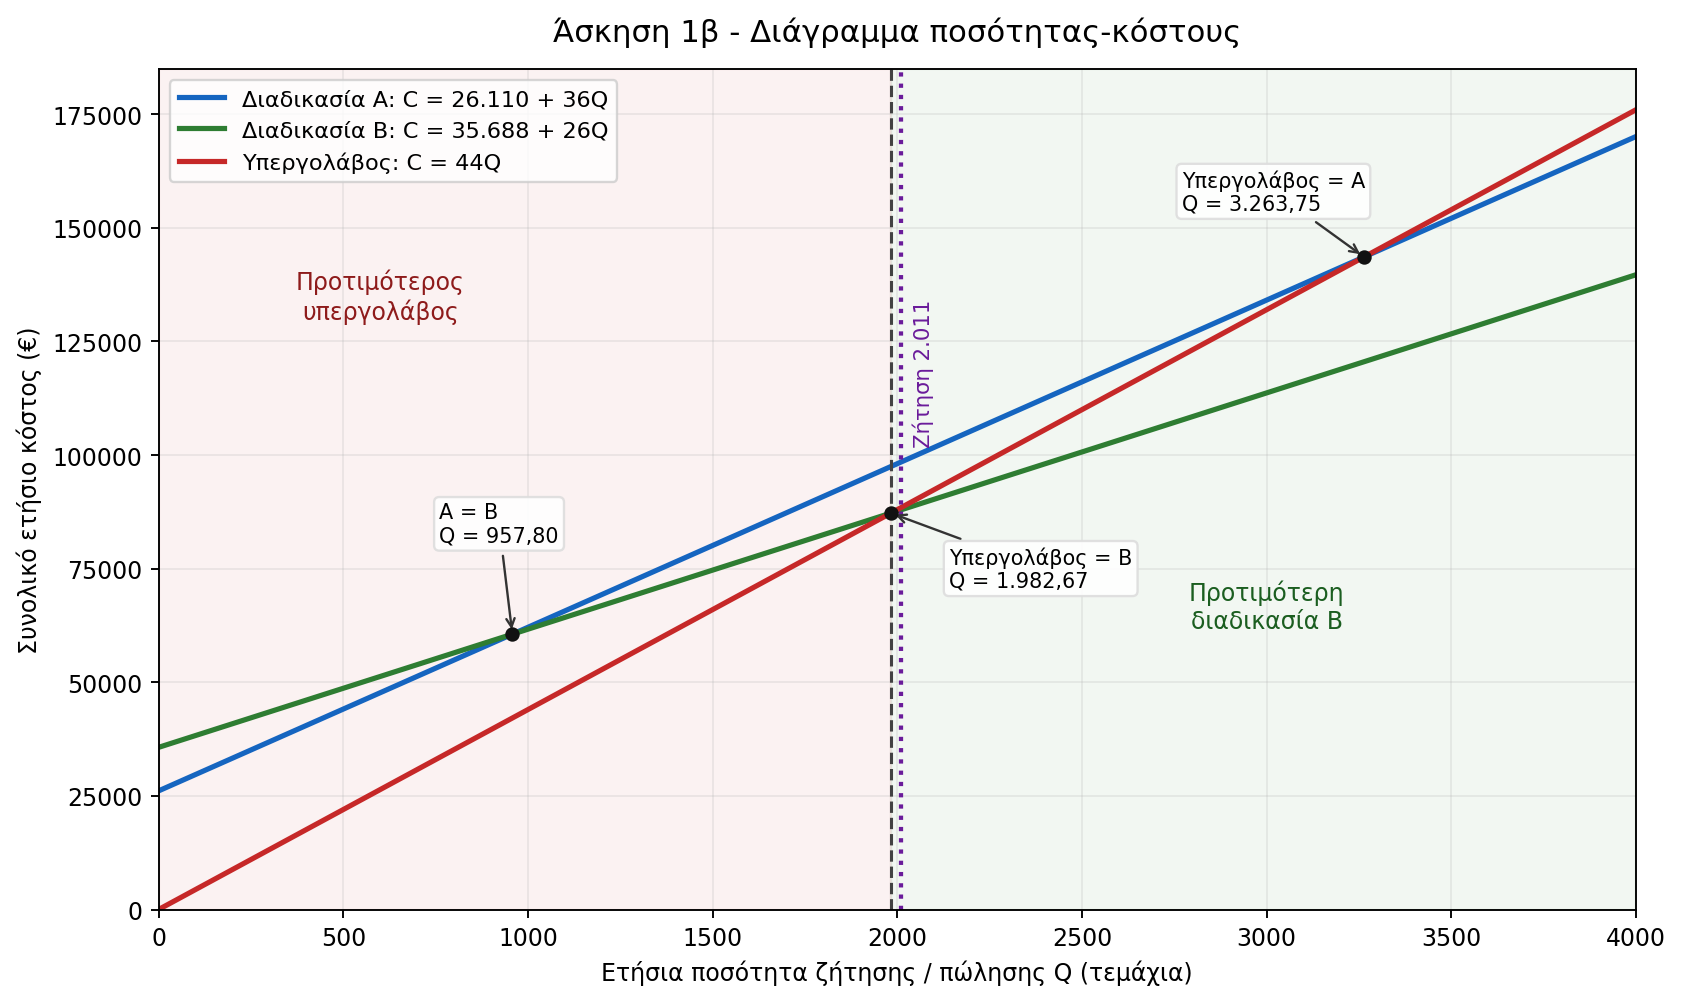
\includegraphics[width=0.95\textwidth]{askisi_1_diagramma_kostous.png}
\caption{Διάγραμμα ποσότητας--κόστους για τις τρεις εναλλακτικές επιλογές}
\end{figure}

Η κόκκινη γραμμή του υπεργολάβου ξεκινά από το μηδέν, επειδή δεν υπάρχει σταθερό κόστος. Όμως ανεβαίνει πιο απότομα, επειδή το μεταβλητό κόστος είναι υψηλό.

Η πράσινη γραμμή της διαδικασίας Β ξεκινά ψηλά, επειδή έχει μεγάλο σταθερό κόστος. Όμως ανεβαίνει πιο αργά, επειδή έχει μικρό μεταβλητό κόστος. Για αυτό, μετά από ένα σημείο, γίνεται η καλύτερη επιλογή.

Η μπλε γραμμή της διαδικασίας Α βρίσκεται ενδιάμεσα, αλλά δεν είναι ποτέ η χαμηλότερη γραμμή. Αυτός είναι ο λόγος που δεν επιλέγεται ως οικονομικά καλύτερη λύση.

\section{Λύση ερωτήματος γ}

\subsection{Τι ζητά το ερώτημα γ}

Το ερώτημα γ μας λέει να υποθέσουμε ότι τελικά η εταιρία επιλέγει τη διαδικασία Α. Επίσης μας λέει ότι οι ετήσιες πωλήσεις είναι:
\[
1.800+x
\]

Με \(x=211\):
\[
Q=1.800+211=2.011
\]

Ζητείται η συμβολή της νέας σειράς καθισμάτων στο ετήσιο κέρδος της εταιρίας. Δηλαδή πρέπει να βρούμε πόσο κέρδος θα φέρει η νέα σειρά, αν χρησιμοποιηθεί η διαδικασία Α και πουληθούν 2.011 τεμάχια.

\subsection{Υπολογισμός εσόδων}

Η τιμή πώλησης είναι 73,10 € ανά τεμάχιο. Για 2.011 τεμάχια, τα συνολικά έσοδα είναι:
\[
R(2.011)=73{,}10\cdot2.011
\]
\[
R(2.011)=147.004{,}10 \text{ €}
\]

\subsection{Υπολογισμός κόστους με τη διαδικασία Α}

Η συνάρτηση κόστους της διαδικασίας Α είναι:
\[
C_A(Q)=26.110+36Q
\]

Για \(Q=2.011\):
\[
C_A(2.011)=26.110+36\cdot2.011
\]
\[
C_A(2.011)=26.110+72.396
\]
\[
C_A(2.011)=98.506 \text{ €}
\]

\subsection{Υπολογισμός κέρδους}

Το κέρδος είναι:
\[
\Pi_A=R-C_A
\]

Άρα:
\[
\Pi_A=147.004{,}10-98.506{,}00
\]
\[
\boxed{\Pi_A=48.498{,}10 \text{ €}}
\]

Ερμηνεία: αν η εταιρία επιλέξει τη διαδικασία Α και πουλήσει 2.011 καθίσματα, η νέα σειρά θα προσθέσει 48.498,10 € στο ετήσιο κέρδος της.

\section{Λύση ερωτήματος δ}

\subsection{Τι ζητά το ερώτημα δ}

Το ερώτημα δ ζητά να κρίνουμε την επιλογή της διαδικασίας Α. Δεν αρκεί να πούμε ότι η διαδικασία Α δίνει κέρδος. Πρέπει να δούμε αν δίνει το μεγαλύτερο δυνατό κέρδος.

Με άλλα λόγια, η ερώτηση είναι:

\begin{quote}
Αφού η ζήτηση είναι 2.011 τεμάχια, ήταν σωστό να επιλεγεί η διαδικασία Α ή υπήρχε οικονομικά καλύτερη επιλογή;
\end{quote}

Για να απαντήσουμε, συγκρίνουμε το συνολικό κόστος όλων των επιλογών για \(Q=2.011\).

\subsection{Κόστος διαδικασίας Α}

Το έχουμε ήδη υπολογίσει:
\[
C_A(2.011)=98.506 \text{ €}
\]

\subsection{Κόστος διαδικασίας Β}

Η συνάρτηση κόστους της διαδικασίας Β είναι:
\[
C_B(Q)=35.688+26Q
\]

Για \(Q=2.011\):
\[
C_B(2.011)=35.688+26\cdot2.011
\]
\[
C_B(2.011)=35.688+52.286
\]
\[
C_B(2.011)=87.974 \text{ €}
\]

\subsection{Κόστος υπεργολάβου}

Η συνάρτηση κόστους του υπεργολάβου είναι:
\[
C_Y(Q)=44Q
\]

Για \(Q=2.011\):
\[
C_Y(2.011)=44\cdot2.011
\]
\[
C_Y(2.011)=88.484 \text{ €}
\]

\subsection{Σύγκριση επιλογών}

\begin{table}[H]
\centering
\caption{Σύγκριση κόστους για ζήτηση 2.011 τεμαχίων}
\begin{tabular}{lc}
\toprule
\textbf{Επιλογή} & \textbf{Συνολικό κόστος} \\
\midrule
Διαδικασία Α & 98.506 € \\
Διαδικασία Β & 87.974 € \\
Υπεργολάβος & 88.484 € \\
\bottomrule
\end{tabular}
\end{table}

Η μικρότερη τιμή είναι 87.974 €, που αντιστοιχεί στη διαδικασία Β. Άρα η διαδικασία Β είναι η καλύτερη επιλογή.

\subsection{Κέρδος με την καλύτερη επιλογή}

Τα έσοδα είναι ίδια, επειδή η τιμή πώλησης δεν αλλάζει:
\[
R(2.011)=147.004{,}10 \text{ €}
\]

Το κέρδος με τη διαδικασία Β είναι:
\[
\Pi_B=R-C_B
\]
\[
\Pi_B=147.004{,}10-87.974{,}00
\]
\[
\boxed{\Pi_B=59.030{,}10 \text{ €}}
\]

\subsection{Πόσο καλύτερη είναι η διαδικασία Β}

Η διαδικασία Α έδινε κέρδος:
\[
\Pi_A=48.498{,}10 \text{ €}
\]

Η διαδικασία Β δίνει κέρδος:
\[
\Pi_B=59.030{,}10 \text{ €}
\]

Η διαφορά είναι:
\[
59.030{,}10-48.498{,}10=10.532{,}00
\]

Άρα:
\[
\boxed{\Pi_B-\Pi_A=10.532{,}00 \text{ €}}
\]

Δηλαδή η διαδικασία Β δίνει 10.532 € μεγαλύτερο ετήσιο κέρδος από τη διαδικασία Α.

\section{Τελικό συμπέρασμα Άσκησης 1}

Η Άσκηση 1 δείχνει ότι μια παραγωγική επιλογή δεν πρέπει να αξιολογείται μόνο από το αν δίνει κέρδος, αλλά από το αν δίνει το μεγαλύτερο δυνατό κέρδος σε σχέση με τις διαθέσιμες εναλλακτικές.

Τα βασικά αποτελέσματα είναι:

\begin{itemize}
    \item Το νεκρό σημείο της διαδικασίας Α είναι 704 τεμάχια.
    \item Το νεκρό σημείο της διαδικασίας Β είναι 758 τεμάχια.
    \item Για ετήσια ζήτηση έως 1.982 τεμάχια συμφέρει ο υπεργολάβος.
    \item Για ετήσια ζήτηση από 1.983 τεμάχια και πάνω συμφέρει η διαδικασία Β.
    \item Η διαδικασία Α δεν είναι ποτέ η φθηνότερη επιλογή.
    \item Για ζήτηση 2.011 τεμαχίων, η διαδικασία Α δίνει κέρδος 48.498,10 €.
    \item Για την ίδια ζήτηση, η διαδικασία Β δίνει κέρδος 59.030,10 €.
    \item Άρα η διαδικασία Β είναι καλύτερη από τη διαδικασία Α κατά 10.532 € ετησίως.
\end{itemize}

Συνεπώς, η τελική διοικητική πρόταση προς την εταιρία Ζ είναι να μην επιλέξει τη διαδικασία Α για την παραγωγή των καθισμάτων. Για τη συγκεκριμένη αναμενόμενη ζήτηση των 2.011 τεμαχίων, η πιο συμφέρουσα επιλογή είναι η διαδικασία Β.

\newpage

\section{Άσκηση 2}

\subsection{Η εκφώνηση με απλά λόγια}

Η εταιρία Ζ, εκτός από καθίσματα γραφείου, παράγει και ξύλινες πολυθρόνες. Για να κατασκευαστεί μία ξύλινη πολυθρόνα χρειάζεται ξυλεία. Η εκφώνηση μάς δίνει τρία βασικά στοιχεία:

\begin{itemize}
    \item Κάθε πολυθρόνα χρειάζεται 18 κιλά ξυλείας.
    \item Η εταιρία παραλαμβάνει κάθε εβδομάδα \(450+6x\) κιλά ξυλείας.
    \item Στο εργοστάσιο υπάρχουν κατά μέσο όρο 120 πολυθρόνες που βρίσκονται σε διάφορες φάσεις κατασκευής.
\end{itemize}

Το ζητούμενο είναι να βρούμε πόσος χρόνος χρειάζεται, κατά μέσο όρο, για να ολοκληρωθεί η παραγωγή μίας πολυθρόνας από τη στιγμή που η ξυλεία είναι διαθέσιμη στο εργοστάσιο.

Με πολύ απλά λόγια, το ερώτημα είναι το εξής:

\begin{quote}
Αν ξέρουμε πόσες πολυθρόνες βρίσκονται μέσα στη διαδικασία παραγωγής και ξέρουμε με τι ρυθμό παράγονται νέες πολυθρόνες, πόσο χρόνο περνά κατά μέσο όρο μία πολυθρόνα μέσα στο σύστημα παραγωγής;
\end{quote}

Αυτό δεν είναι ερώτημα κόστους, όπως η Άσκηση 1. Είναι ερώτημα ροής παραγωγής. Μας ενδιαφέρει δηλαδή η κίνηση των προϊόντων μέσα στο εργοστάσιο και ο χρόνος που απαιτείται για να μετατραπεί η διαθέσιμη πρώτη ύλη σε τελικό προϊόν.

\subsection{Τα δεδομένα της άσκησης}

Έχουμε:

\[
x=211
\]

Η ποσότητα ξυλείας που παραλαμβάνει η εταιρία κάθε εβδομάδα είναι:
\[
450+6x
\]

Κάθε ξύλινη πολυθρόνα χρειάζεται:
\[
18 \text{ kg ξυλείας}
\]

Ο μέσος αριθμός πολυθρόνων που βρίσκονται μέσα στο εργοστάσιο, σε διάφορες φάσεις κατασκευής, είναι:
\[
120 \text{ πολυθρόνες}
\]

Αυτές οι 120 πολυθρόνες δεν είναι απαραίτητα έτοιμες. Μπορεί κάποιες να βρίσκονται στην αρχή της παραγωγής, κάποιες στη μέση και κάποιες κοντά στο τέλος. Όλες μαζί αποτελούν το μέσο απόθεμα σε παραγωγή.

\section{Θεωρητικό υπόβαθρο Άσκησης 2}

\subsection{Τι είναι πρώτη ύλη}

Πρώτη ύλη είναι το υλικό που χρησιμοποιείται για να παραχθεί ένα προϊόν. Στην παρούσα άσκηση, η πρώτη ύλη είναι η ξυλεία.

Η εκφώνηση λέει ότι για κάθε πολυθρόνα χρειάζονται 18 κιλά ξυλείας. Άρα, αν έχουμε διαθέσιμα 18 κιλά ξυλείας, μπορούμε θεωρητικά να φτιάξουμε 1 πολυθρόνα. Αν έχουμε 180 κιλά ξυλείας, μπορούμε να φτιάξουμε:
\[
\frac{180}{18}=10 \text{ πολυθρόνες}
\]

Γενικά:
\[
\text{Πολυθρόνες που μπορούν να παραχθούν}=
\frac{\text{Διαθέσιμη ξυλεία}}{\text{Ξυλεία ανά πολυθρόνα}}
\]

\subsection{Τι είναι ρυθμός παραγωγής}

Ο ρυθμός παραγωγής δείχνει πόσες μονάδες προϊόντος παράγονται σε μία χρονική περίοδο. Για παράδειγμα, αν ένα εργοστάσιο παράγει 100 πολυθρόνες την εβδομάδα, τότε ο ρυθμός παραγωγής του είναι:
\[
100 \text{ πολυθρόνες/εβδομάδα}
\]

Στην άσκηση δεν μας δίνεται απευθείας ο ρυθμός παραγωγής. Μας δίνεται όμως πόση ξυλεία έρχεται κάθε εβδομάδα και πόση ξυλεία χρειάζεται κάθε πολυθρόνα. Άρα μπορούμε να υπολογίσουμε πόσες πολυθρόνες μπορεί να υποστηρίξει αυτή η εβδομαδιαία παροχή ξυλείας.

\subsection{Τι είναι απόθεμα σε παραγωγή}

Το απόθεμα σε παραγωγή είναι τα προϊόντα που έχουν ξεκινήσει να κατασκευάζονται, αλλά δεν έχουν ολοκληρωθεί ακόμη. Στα αγγλικά συχνά λέγεται \textenglish{Work In Process} ή \textenglish{Work In Progress}, δηλαδή WIP.

Στην άσκηση, το WIP είναι:
\[
WIP=120 \text{ πολυθρόνες}
\]

Αυτό σημαίνει ότι, κατά μέσο όρο, μέσα στο εργοστάσιο υπάρχουν 120 πολυθρόνες που δεν είναι τελικά προϊόντα, αλλά βρίσκονται κάπου μέσα στη διαδικασία κατασκευής.

\subsection{Τι είναι χρόνος ροής}

Ο χρόνος ροής είναι ο μέσος χρόνος που περνά ένα προϊόν μέσα στο σύστημα παραγωγής. Στην άσκηση, είναι ο χρόνος από τη στιγμή που η ξυλεία είναι διαθέσιμη στο εργοστάσιο μέχρι τη στιγμή που ολοκληρώνεται η πολυθρόνα.

Αν ο χρόνος ροής είναι μεγάλος, αυτό σημαίνει ότι τα προϊόντα μένουν πολλή ώρα μέσα στο εργοστάσιο πριν ολοκληρωθούν. Αν είναι μικρός, η παραγωγική διαδικασία είναι πιο γρήγορη.

\subsection{Ο νόμος του Little}

Για να λύσουμε την άσκηση χρησιμοποιούμε τον νόμο του Little. Είναι ένας πολύ βασικός νόμος στη διοίκηση παραγωγής και στη μελέτη συστημάτων ροής.

Ο νόμος του Little λέει:
\begin{align*}
\text{Μέσο απόθεμα στο σύστημα}
&= \text{Ρυθμός ροής} \\
&\quad \cdot \text{Μέσος χρόνος παραμονής στο σύστημα}
\end{align*}

Συμβολικά:
\[
L=\lambda W
\]

όπου:

\begin{itemize}
    \item \(L\) είναι ο μέσος αριθμός μονάδων μέσα στο σύστημα.
    \item \(\lambda\) είναι ο ρυθμός ροής, δηλαδή πόσες μονάδες ολοκληρώνονται ανά χρονική περίοδο.
    \item \(W\) είναι ο μέσος χρόνος που περνά κάθε μονάδα μέσα στο σύστημα.
\end{itemize}

Στη δική μας άσκηση:

\begin{itemize}
    \item Το \(L\) είναι οι 120 πολυθρόνες που βρίσκονται κατά μέσο όρο μέσα στην παραγωγή.
    \item Το \(\lambda\) είναι ο εβδομαδιαίος ρυθμός παραγωγής πολυθρόνων.
    \item Το \(W\) είναι ο μέσος χρόνος ολοκλήρωσης μίας πολυθρόνας.
\end{itemize}

Εμείς θέλουμε να βρούμε τον χρόνο \(W\). Άρα λύνουμε τον τύπο ως προς \(W\):
\[
W=\frac{L}{\lambda}
\]

Με λόγια:

\begin{quote}
Ο μέσος χρόνος ολοκλήρωσης ισούται με τον μέσο αριθμό προϊόντων που βρίσκονται μέσα στην παραγωγή, διαιρεμένο με τον ρυθμό παραγωγής.
\end{quote}

\section{Λύση Άσκησης 2 βήμα προς βήμα}

\subsection{Βήμα 1: Υπολογισμός εβδομαδιαίας ξυλείας}

Η εκφώνηση λέει ότι η εταιρία προμηθεύεται κάθε εβδομάδα:
\[
450+6x
\]
κιλά ξυλείας.

Επειδή:
\[
x=211
\]

έχουμε:
\[
450+6\cdot211
\]

Υπολογίζουμε πρώτα τον πολλαπλασιασμό:
\[
6\cdot211=1.266
\]

Άρα:
\[
450+1.266=1.716
\]

Επομένως, η εταιρία παραλαμβάνει κάθε εβδομάδα:
\[
\boxed{1.716 \text{ kg ξυλείας/εβδομάδα}}
\]

\subsection{Βήμα 2: Μετατροπή της ξυλείας σε αριθμό πολυθρόνων}

Ξέρουμε ότι κάθε πολυθρόνα χρειάζεται 18 kg ξυλείας. Άρα, για να βρούμε πόσες πολυθρόνες μπορεί να παραχθούν με 1.716 kg ξυλείας, διαιρούμε:
\[
\frac{1.716}{18}
\]

Ο υπολογισμός δίνει:
\[
\frac{1.716}{18}=95{,}33
\]

Άρα ο ρυθμός παραγωγής, με βάση τη διαθέσιμη ξυλεία, είναι:
\[
\boxed{95{,}33 \text{ πολυθρόνες/εβδομάδα}}
\]

Αυτό σημαίνει ότι η εβδομαδιαία παροχή ξυλείας επαρκεί, κατά μέσο όρο, για την παραγωγή περίπου 95,33 πολυθρόνων την εβδομάδα.

Στην πράξη, δεν μπορεί να παραχθεί το 0,33 μιας πολυθρόνας ως τελικό ακέραιο προϊόν. Όμως στους υπολογισμούς ρυθμού παραγωγής χρησιμοποιούμε δεκαδικούς αριθμούς, επειδή μιλάμε για μέσο ρυθμό σε βάθος χρόνου.

\subsection{Βήμα 3: Αναγνώριση του μέσου αποθέματος σε παραγωγή}

Η εκφώνηση λέει ότι στο εργοστάσιο υπάρχουν διαχρονικά, κατά μέσο όρο, 120 ξύλινες πολυθρόνες σε διάφορες φάσεις κατασκευής.

Άρα:
\[
L=120
\]

Αυτό είναι το μέσο απόθεμα σε παραγωγή. Δεν σημαίνει ότι ακριβώς κάθε στιγμή υπάρχουν πάντα 120 πολυθρόνες. Σημαίνει ότι αν παρατηρούσαμε το εργοστάσιο για μεγάλο χρονικό διάστημα, ο μέσος αριθμός ημιτελών πολυθρόνων θα ήταν 120.

\subsection{Βήμα 4: Εφαρμογή του νόμου του Little}

Ο νόμος του Little είναι:
\[
L=\lambda W
\]

Θέλουμε τον χρόνο \(W\), οπότε:
\[
W=\frac{L}{\lambda}
\]

Αντικαθιστούμε:
\[
L=120
\]
\[
\lambda=95{,}33
\]

Άρα:
\[
W=\frac{120}{95{,}33}
\]

Ο υπολογισμός δίνει:
\[
W=1{,}2587 \text{ εβδομάδες}
\]

Στρογγυλοποιημένα:
\[
\boxed{W=1{,}26 \text{ εβδομάδες}}
\]

\subsection{Βήμα 5: Μετατροπή σε ημέρες}

Το αποτέλεσμα σε εβδομάδες είναι σωστό, επειδή ο ρυθμός παραγωγής ήταν σε πολυθρόνες ανά εβδομάδα. Όμως πολλές φορές είναι πιο εύκολο να καταλάβουμε τον χρόνο σε ημέρες.

Μία εβδομάδα έχει 7 ημέρες. Άρα:
\[
1{,}2587\cdot7=8{,}811
\]

Στρογγυλοποιημένα:
\[
\boxed{8{,}81 \text{ ημέρες}}
\]

\section{Ερμηνεία του αποτελέσματος}

Το αποτέλεσμα:
\[
1{,}26 \text{ εβδομάδες}
\]
ή:
\[
8{,}81 \text{ ημέρες}
\]
σημαίνει ότι μία πολυθρόνα χρειάζεται, κατά μέσο όρο, περίπου 8,81 ημέρες για να ολοκληρωθεί από τη στιγμή που η ξυλεία είναι διαθέσιμη στο εργοστάσιο.

Είναι σημαντικό να προσέξουμε ότι αυτός δεν είναι απαραίτητα ο καθαρός χρόνος εργασίας πάνω στην πολυθρόνα. Περιλαμβάνει όλο τον χρόνο που η πολυθρόνα βρίσκεται μέσα στο σύστημα παραγωγής. Δηλαδή μπορεί να περιλαμβάνει:

\begin{itemize}
    \item χρόνο πραγματικής κατεργασίας,
    \item χρόνο αναμονής ανάμεσα σε στάδια,
    \item χρόνο μεταφοράς μέσα στο εργοστάσιο,
    \item χρόνο που το προϊόν βρίσκεται σε ενδιάμεση κατάσταση μέχρι να προχωρήσει στο επόμενο στάδιο.
\end{itemize}

Γι' αυτό ο χρόνος ροής είναι συχνά μεγαλύτερος από τον καθαρό χρόνο επεξεργασίας. Μας ενδιαφέρει διοικητικά επειδή δείχνει πόσο γρήγορα το σύστημα μετατρέπει την πρώτη ύλη σε τελικό προϊόν.

\section{Τελικό συμπέρασμα Άσκησης 2}

Η εταιρία λαμβάνει 1.716 kg ξυλείας την εβδομάδα. Επειδή κάθε πολυθρόνα χρειάζεται 18 kg, ο μέσος ρυθμός παραγωγής είναι:
\[
95{,}33 \text{ πολυθρόνες/εβδομάδα}
\]

Στο εργοστάσιο υπάρχουν κατά μέσο όρο 120 πολυθρόνες σε εξέλιξη. Με τον νόμο του Little:
\[
W=\frac{120}{95{,}33}=1{,}26 \text{ εβδομάδες}
\]

Άρα ο μέσος χρόνος που απαιτείται για την ολοκλήρωση μίας ξύλινης πολυθρόνας είναι:
\[
\boxed{1{,}26 \text{ εβδομάδες ή περίπου } 8{,}81 \text{ ημέρες}}
\]

Η διοικητική ερμηνεία είναι ότι, με τον σημερινό ρυθμό εισροής ξυλείας και με 120 πολυθρόνες κατά μέσο όρο μέσα στην παραγωγή, κάθε πολυθρόνα παραμένει στο παραγωγικό σύστημα περίπου εννέα ημέρες πριν ολοκληρωθεί.

\newpage

\section{Άσκηση 3}

\subsection{Η εκφώνηση με απλά λόγια}

Στην Άσκηση 3 δεν ασχολούμαστε πλέον με παραγωγή μέσα σε ένα εργοστάσιο, αλλά με μεταφορά προϊόντων μέσα σε μια εφοδιαστική αλυσίδα.

Η εφοδιαστική αλυσίδα έχει:

\begin{itemize}
    \item δύο εργοστάσια, δηλαδή δύο σημεία από τα οποία ξεκινούν τα προϊόντα,
    \item τέσσερις αποθήκες, δηλαδή τέσσερα σημεία στα οποία πρέπει να φτάσουν τα προϊόντα,
    \item διαφορετικά κόστη μεταφοράς από κάθε εργοστάσιο προς κάθε αποθήκη.
\end{itemize}

Το ερώτημα είναι:

\begin{quote}
Πόσες μονάδες πρέπει να στείλει κάθε εργοστάσιο σε κάθε αποθήκη, ώστε να καλυφθούν όλες οι ζητήσεις με το μικρότερο δυνατό συνολικό κόστος μεταφοράς;
\end{quote}

Άρα δεν μας ενδιαφέρει απλώς να βρούμε μια οποιαδήποτε λύση. Θέλουμε τη βέλτιστη λύση, δηλαδή εκείνη που έχει το ελάχιστο συνολικό κόστος.

Η εκφώνηση ζητά συγκεκριμένα να ακολουθήσουμε δύο στάδια:

\begin{enumerate}
    \item Πρώτα να βρούμε μια αρχική εφικτή λύση με τη μέθοδο της ΒΔ γωνίας.
    \item Μετά να βελτιώσουμε και να ελέγξουμε τη λύση με τη μέθοδο MODI.
\end{enumerate}

\subsection{Τι σημαίνει εφικτή και τι σημαίνει βέλτιστη λύση}

Μια λύση λέγεται εφικτή όταν σέβεται όλους τους περιορισμούς του προβλήματος. Δηλαδή:

\begin{itemize}
    \item κανένα εργοστάσιο δεν στέλνει περισσότερες μονάδες από όσες μπορεί να διαθέσει,
    \item κάθε αποθήκη παραλαμβάνει ακριβώς όση ποσότητα ζητά,
    \item όλες οι ποσότητες μεταφοράς είναι μη αρνητικές.
\end{itemize}

Μια λύση λέγεται βέλτιστη όταν, εκτός από εφικτή, έχει και το μικρότερο δυνατό συνολικό κόστος.

Η μέθοδος της ΒΔ γωνίας μάς δίνει γρήγορα μια αρχική εφικτή λύση. Δεν εγγυάται όμως ότι αυτή η λύση είναι η φθηνότερη. Για αυτό στη συνέχεια εφαρμόζεται η μέθοδος MODI, η οποία ελέγχει αν υπάρχει τρόπος να μειωθεί το κόστος.

\section{Δεδομένα Άσκησης 3 μετά τη στρογγυλοποίηση}

\subsection{Δυναμικότητες εργοστασίων}

Δίνεται ότι το εργοστάσιο 1 έχει μηνιαία δυναμικότητα:
\[
150 \text{ μονάδες}
\]

Το εργοστάσιο 2 έχει μηνιαία δυναμικότητα:
\[
100+\frac{x}{3}
\]

Με \(x=211\):
\[
100+\frac{211}{3}=100+70{,}33=170{,}33
\]

Η εκφώνηση λέει ότι όλες οι δεκαδικές τιμές στρογγυλοποιούνται στον πλησιέστερο ακέραιο. Άρα:
\[
170{,}33 \simeq 170
\]

Επομένως:
\[
\boxed{\text{Δυναμικότητα εργοστασίου 1}=150}
\]
\[
\boxed{\text{Δυναμικότητα εργοστασίου 2}=170}
\]

Η συνολική δυναμικότητα των δύο εργοστασίων είναι:
\[
150+170=320 \text{ μονάδες/μήνα}
\]

\subsection{Ζητήσεις αποθηκών}

Οι ζητήσεις των αποθηκών Α, Β και Γ δίνονται απευθείας:
\[
A=50,\quad B=60,\quad \Gamma=70
\]

Η ζήτηση της αποθήκης Δ είναι:
\[
60+\frac{x}{5}
\]

Με \(x=211\):
\[
60+\frac{211}{5}=60+42{,}20=102{,}20
\]

Στρογγυλοποίηση:
\[
102{,}20 \simeq 102
\]

Άρα:
\[
\boxed{\Delta=102}
\]

Η συνολική ζήτηση είναι:
\[
50+60+70+102=282 \text{ μονάδες/μήνα}
\]

\subsection{Σύγκριση δυναμικότητας και ζήτησης}

Έχουμε:
\[
\text{Συνολική δυναμικότητα}=320
\]
\[
\text{Συνολική ζήτηση}=282
\]

Η δυναμικότητα είναι μεγαλύτερη από τη ζήτηση:
\[
320>282
\]

Η διαφορά είναι:
\[
320-282=38
\]

Αυτό σημαίνει ότι τα εργοστάσια μπορούν να παράγουν ή να διαθέσουν 38 μονάδες περισσότερες από όσες ζητούν οι πραγματικές αποθήκες.

\section{Θεωρητικό υπόβαθρο Άσκησης 3}

\subsection{Τι είναι το πρότυπο μεταφοράς}

Το πρότυπο μεταφοράς είναι ένα μοντέλο που χρησιμοποιείται όταν έχουμε προϊόντα που ξεκινούν από κάποια σημεία προσφοράς και πρέπει να σταλούν σε κάποια σημεία ζήτησης.

Στην άσκηση:

\begin{itemize}
    \item σημεία προσφοράς είναι τα δύο εργοστάσια,
    \item σημεία ζήτησης είναι οι τέσσερις αποθήκες,
    \item κόστος μεταφοράς είναι το κόστος για να μεταφερθεί μία μονάδα από ένα εργοστάσιο σε μία αποθήκη.
\end{itemize}

Αν συμβολίσουμε με \(x_{ij}\) την ποσότητα που μεταφέρεται από το εργοστάσιο \(i\) στην αποθήκη \(j\), τότε το συνολικό κόστος είναι:
\[
\text{Συνολικό κόστος}=\sum c_{ij}x_{ij}
\]

όπου \(c_{ij}\) είναι το μοναδιαίο κόστος μεταφοράς από το εργοστάσιο \(i\) στην αποθήκη \(j\).

\subsection{Τι σημαίνει ισορροπημένο πρόβλημα μεταφοράς}

Ένα πρόβλημα μεταφοράς λέγεται ισορροπημένο όταν:
\[
\text{Συνολική προσφορά}=\text{Συνολική ζήτηση}
\]

Εδώ όμως έχουμε:
\[
320 \neq 282
\]

Άρα το πρόβλημα δεν είναι αρχικά ισορροπημένο.

Όταν η προσφορά είναι μεγαλύτερη από τη ζήτηση, προσθέτουμε μία εικονική αποθήκη. Η εικονική αποθήκη δεν είναι πραγματική αποθήκη. Είναι ένας τεχνικός τρόπος να καταγράψουμε την αχρησιμοποίητη δυναμικότητα.

Η ζήτηση της εικονικής αποθήκης είναι:
\[
38 \text{ μονάδες}
\]

Το κόστος μεταφοράς προς την εικονική αποθήκη είναι 0, επειδή στην πραγματικότητα αυτές οι μονάδες δεν μεταφέρονται πουθενά. Απλώς μένουν αχρησιμοποίητες.

\subsection{Τι είναι η μέθοδος της ΒΔ γωνίας}

Η μέθοδος της ΒΔ γωνίας είναι ένας απλός τρόπος για να φτιάξουμε μια αρχική εφικτή λύση.

Ονομάζεται έτσι επειδή ξεκινάμε από το πάνω αριστερό κελί του πίνακα, δηλαδή από τη βορειοδυτική γωνία. Στη συνέχεια γεμίζουμε τον πίνακα μετακινώντας μας δεξιά ή κάτω, ανάλογα με το ποια γραμμή ή στήλη ικανοποιείται.

Η λογική είναι:

\begin{enumerate}
    \item Ξεκινάμε από το πρώτο διαθέσιμο κελί.
    \item Βάζουμε εκεί όσο το δυνατόν μεγαλύτερη ποσότητα.
    \item Αν καλυφθεί η ζήτηση μιας αποθήκης, μετακινούμαστε στην επόμενη στήλη.
    \item Αν εξαντληθεί η προσφορά ενός εργοστασίου, μετακινούμαστε στην επόμενη γραμμή.
    \item Συνεχίζουμε μέχρι να καλυφθούν όλες οι ζητήσεις.
\end{enumerate}

Η μέθοδος αυτή δεν κοιτάζει τα κόστη. Για αυτό μπορεί να δώσει λύση που είναι εφικτή αλλά όχι βέλτιστη.

\subsection{Τι είναι η μέθοδος MODI}

Η μέθοδος MODI χρησιμοποιείται για να ελέγξουμε αν μια λύση μεταφοράς είναι βέλτιστη και, αν δεν είναι, να τη βελτιώσουμε.

Η βασική ιδέα είναι η εξής:

\begin{itemize}
    \item Υπολογίζουμε ορισμένες βοηθητικές τιμές για τις γραμμές και τις στήλες του πίνακα.
    \item Με αυτές τις τιμές βρίσκουμε αν κάποια κενή θέση θα μπορούσε να μειώσει το συνολικό κόστος.
    \item Αν υπάρχει τέτοια θέση, κάνουμε μετακίνηση ποσοτήτων σε κλειστό βρόχο.
    \item Επαναλαμβάνουμε μέχρι να μην υπάρχει άλλη μείωση κόστους.
\end{itemize}

Για κάθε μη βασική, δηλαδή κενή, θέση υπολογίζουμε έναν δείκτη βελτίωσης:
\[
\Delta_{ij}=c_{ij}-u_i-v_j
\]

Σε πρόβλημα ελαχιστοποίησης κόστους:

\begin{itemize}
    \item Αν όλοι οι δείκτες \(\Delta_{ij}\) είναι μη αρνητικοί, η λύση είναι βέλτιστη.
    \item Αν υπάρχει αρνητικός δείκτης, τότε η λύση μπορεί να βελτιωθεί.
\end{itemize}

Ο λόγος είναι ότι ο δείκτης \(\Delta_{ij}\) δείχνει πόσο θα αλλάξει το συνολικό κόστος αν αρχίσουμε να χρησιμοποιούμε το αντίστοιχο κενό κελί. Σε πρόβλημα ελαχιστοποίησης, αρνητικός δείκτης σημαίνει μείωση κόστους. Για παράδειγμα, αν \(\Delta_{ij}=-5\), τότε κάθε μονάδα που μπαίνει σε αυτόν τον βρόχο μειώνει το συνολικό κόστος κατά 5 μονάδες κόστους.

Όταν υπάρχουν περισσότεροι από ένας αρνητικοί δείκτες, συνήθως επιλέγουμε αυτόν με την αλγεβρικά μικρότερη τιμή, δηλαδή τον πιο αρνητικό. Αυτό γίνεται επειδή ο πιο αρνητικός δείκτης υπόσχεται τη μεγαλύτερη μείωση κόστους ανά μονάδα μετακίνησης. Δεν είναι ότι οι άλλοι αρνητικοί δείκτες είναι λάθος επιλογές· και αυτοί θα μπορούσαν να βελτιώσουν τη λύση. Όμως ο πιο αρνητικός δείκτης είναι η πιο ισχυρή άμεση βελτίωση και συνήθως οδηγεί γρηγορότερα στη βέλτιστη λύση.

\section{Ισορροπημένος πίνακας μεταφοράς}

Αφού προσθέσουμε την εικονική αποθήκη, ο πίνακας γίνεται:

\begin{table}[H]
\centering
\caption{Ισορροπημένος πίνακας μεταφοράς}
\small
\begin{tabular}{lrrrrrr}
\toprule
 & \textbf{Α} & \textbf{Β} & \textbf{Γ} & \textbf{Δ} & \textbf{Εικονική Ε} & \textbf{Προσφορά} \\
\midrule
Εργοστάσιο 1 & 14 & 20 & 14 & 18 & 0 & 150 \\
Εργοστάσιο 2 & 15 & 18 & 17 & 16 & 0 & 170 \\
\midrule
Ζήτηση & 50 & 60 & 70 & 102 & 38 & 320 \\
\bottomrule
\end{tabular}
\end{table}

Οι αριθμοί μέσα στον πίνακα, εκτός από την τελευταία γραμμή και την τελευταία στήλη, είναι μοναδιαία κόστη μεταφοράς. Για παράδειγμα, το κόστος από το εργοστάσιο 1 προς την αποθήκη Β είναι 20 ανά μονάδα.

\section{Αρχική λύση με τη μέθοδο της ΒΔ γωνίας}

\subsection{Βήμα 1: Από εργοστάσιο 1 προς αποθήκη Α}

Ξεκινάμε από το πάνω αριστερό κελί: εργοστάσιο 1 προς αποθήκη Α.

Το εργοστάσιο 1 έχει διαθέσιμες 150 μονάδες και η αποθήκη Α ζητά 50 μονάδες. Άρα μπορούμε να στείλουμε:
\[
\min(150,50)=50
\]

Στέλνουμε:
\[
x_{1A}=50
\]

Η αποθήκη Α καλύφθηκε πλήρως. Στο εργοστάσιο 1 μένουν:
\[
150-50=100
\]

\subsection{Βήμα 2: Από εργοστάσιο 1 προς αποθήκη Β}

Η επόμενη αποθήκη είναι η Β. Ζητά 60 μονάδες. Το εργοστάσιο 1 έχει ακόμη 100 μονάδες διαθέσιμες.

Άρα:
\[
\min(100,60)=60
\]

Στέλνουμε:
\[
x_{1B}=60
\]

Η αποθήκη Β καλύφθηκε. Στο εργοστάσιο 1 μένουν:
\[
100-60=40
\]

\subsection{Βήμα 3: Από εργοστάσιο 1 προς αποθήκη Γ}

Η αποθήκη Γ ζητά 70 μονάδες, αλλά το εργοστάσιο 1 έχει μόνο 40 μονάδες διαθέσιμες.

Άρα:
\[
\min(40,70)=40
\]

Στέλνουμε:
\[
x_{1\Gamma}=40
\]

Το εργοστάσιο 1 εξαντλήθηκε. Η αποθήκη Γ δεν έχει καλυφθεί πλήρως, γιατί ζητούσε 70 και πήρε 40. Άρα απομένουν:
\[
70-40=30
\]

\subsection{Βήμα 4: Από εργοστάσιο 2 προς αποθήκη Γ}

Περνάμε στο εργοστάσιο 2. Η αποθήκη Γ χρειάζεται ακόμη 30 μονάδες.

Το εργοστάσιο 2 έχει 170 μονάδες διαθέσιμες. Άρα:
\[
\min(170,30)=30
\]

Στέλνουμε:
\[
x_{2\Gamma}=30
\]

Η αποθήκη Γ καλύφθηκε. Στο εργοστάσιο 2 μένουν:
\[
170-30=140
\]

\subsection{Βήμα 5: Από εργοστάσιο 2 προς αποθήκη Δ}

Η αποθήκη Δ ζητά 102 μονάδες. Το εργοστάσιο 2 έχει 140 διαθέσιμες.

Άρα:
\[
\min(140,102)=102
\]

Στέλνουμε:
\[
x_{2\Delta}=102
\]

Η αποθήκη Δ καλύφθηκε. Στο εργοστάσιο 2 μένουν:
\[
140-102=38
\]

\subsection{Βήμα 6: Από εργοστάσιο 2 προς εικονική αποθήκη}

Έχουν καλυφθεί όλες οι πραγματικές αποθήκες, αλλά στο εργοστάσιο 2 μένουν 38 μονάδες δυναμικότητας. Αυτές πηγαίνουν στην εικονική αποθήκη:
\[
x_{2E}=38
\]

Αυτό σημαίνει ότι 38 μονάδες δυναμικότητας δεν χρησιμοποιούνται για πραγματική μεταφορά.

\subsection{Πίνακας αρχικής λύσης}

\begin{table}[H]
\centering
\caption{Αρχική λύση με τη μέθοδο της ΒΔ γωνίας}
\small
\begin{tabular}{lrrrrrr}
\toprule
 & \textbf{Α} & \textbf{Β} & \textbf{Γ} & \textbf{Δ} & \textbf{Εικονική Ε} & \textbf{Προσφορά} \\
\midrule
Εργοστάσιο 1 & 50 & 60 & 40 & 0 & 0 & 150 \\
Εργοστάσιο 2 & 0 & 0 & 30 & 102 & 38 & 170 \\
\midrule
Ζήτηση & 50 & 60 & 70 & 102 & 38 & 320 \\
\bottomrule
\end{tabular}
\end{table}

\subsection{Κόστος αρχικής λύσης}

Υπολογίζουμε το κόστος πολλαπλασιάζοντας κάθε ποσότητα με το αντίστοιχο μοναδιαίο κόστος:

\[
C=50\cdot14+60\cdot20+40\cdot14+30\cdot17+102\cdot16+38\cdot0
\]

Άρα:
\[
C=700+1.200+560+510+1.632+0
\]

\[
\boxed{C=4.602}
\]

Η αρχική λύση είναι εφικτή, επειδή καλύπτει όλες τις ζητήσεις και δεν ξεπερνά τις προσφορές. Δεν ξέρουμε όμως ακόμη αν είναι βέλτιστη.

\section{Έλεγχος και βελτίωση με MODI}

\subsection{Πρώτη εφαρμογή MODI}

Στη μέθοδο MODI βρίσκουμε τιμές \(u_i\) για τις γραμμές και \(v_j\) για τις στήλες. Για κάθε βασική θέση, δηλαδή για κάθε θέση που έχει θετική ποσότητα, ισχύει:
\[
c_{ij}=u_i+v_j
\]

Οι βασικές θέσεις είναι τα κελιά στα οποία υπάρχει μεταφορά ποσότητας. Στην αρχική λύση της ΒΔ γωνίας οι βασικές θέσεις είναι:
\[
x_{1A},\quad x_{1B},\quad x_{1\Gamma},\quad x_{2\Gamma},\quad x_{2\Delta},\quad x_{2E}
\]

Γιατί χρησιμοποιούμε μόνο αυτές; Επειδή αυτές είναι οι διαδρομές που συμμετέχουν στην τρέχουσα λύση. Η MODI πρώτα ``διαβάζει'' την τρέχουσα λύση από τα γεμάτα κελιά και μετά εξετάζει αν συμφέρει να μπει κάποιο κενό κελί.

Για να ξεκινήσει ο υπολογισμός, θέτουμε αυθαίρετα:
\[
u_1=0
\]

Μπορούμε να θέσουμε αυθαίρετα ένα από τα \(u_i\) ή \(v_j\) ίσο με 0, γιατί το σύστημα των εξισώσεων έχει μία ελευθερία. Δεν έχει σημασία ποιο θα διαλέξουμε. Συνήθως διαλέγουμε το \(u_1=0\), επειδή είναι το πιο απλό.

Τώρα γράφουμε μία εξίσωση για κάθε βασική θέση.

Για το κελί \(x_{1A}\), το κόστος είναι \(c_{1A}=14\). Άρα:
\[
u_1+v_A=14
\]
Επειδή \(u_1=0\):
\[
0+v_A=14 \Rightarrow v_A=14
\]

Για το κελί \(x_{1B}\), το κόστος είναι \(c_{1B}=20\):
\[
u_1+v_B=20
\]
\[
0+v_B=20 \Rightarrow v_B=20
\]

Για το κελί \(x_{1\Gamma}\), το κόστος είναι \(c_{1\Gamma}=14\):
\[
u_1+v_\Gamma=14
\]
\[
0+v_\Gamma=14 \Rightarrow v_\Gamma=14
\]

Για το κελί \(x_{2\Gamma}\), το κόστος είναι \(c_{2\Gamma}=17\):
\[
u_2+v_\Gamma=17
\]
Επειδή ήδη βρήκαμε \(v_\Gamma=14\):
\[
u_2+14=17 \Rightarrow u_2=3
\]

Για το κελί \(x_{2\Delta}\), το κόστος είναι \(c_{2\Delta}=16\):
\[
u_2+v_\Delta=16
\]
Επειδή \(u_2=3\):
\[
3+v_\Delta=16 \Rightarrow v_\Delta=13
\]

Για το κελί \(x_{2E}\), το κόστος προς την εικονική αποθήκη είναι \(c_{2E}=0\):
\[
u_2+v_E=0
\]
\[
3+v_E=0 \Rightarrow v_E=-3
\]

Άρα οι συντελεστές της πρώτης εφαρμογής MODI είναι:
\[
u_1=0,\quad u_2=3
\]
\[
v_A=14,\quad v_B=20,\quad v_\Gamma=14,\quad v_\Delta=13,\quad v_E=-3
\]

Τώρα υπολογίζουμε τους δείκτες βελτίωσης για τις κενές θέσεις:
\[
\Delta_{ij}=c_{ij}-u_i-v_j
\]

Οι κενές θέσεις της αρχικής λύσης είναι:
\[
x_{1\Delta},\quad x_{1E},\quad x_{2A},\quad x_{2B}
\]

Για τη θέση \(x_{1\Delta}\):
\[
\Delta_{1\Delta}=c_{1\Delta}-u_1-v_\Delta
\]
\[
\Delta_{1\Delta}=18-0-13=5
\]

Για τη θέση \(x_{1E}\):
\[
\Delta_{1E}=c_{1E}-u_1-v_E
\]
\[
\Delta_{1E}=0-0-(-3)=3
\]

Για τη θέση \(x_{2A}\):
\[
\Delta_{2A}=c_{2A}-u_2-v_A
\]
\[
\Delta_{2A}=15-3-14=-2
\]

Για τη θέση \(x_{2B}\):
\[
\Delta_{2B}=c_{2B}-u_2-v_B
\]
\[
\Delta_{2B}=18-3-20=-5
\]

Συνοπτικά:

\begin{table}[H]
\centering
\caption{Δείκτες βελτίωσης στην πρώτη εφαρμογή MODI}
\begin{tabular}{lc}
\toprule
\textbf{Μη βασική μεταβλητή} & \(\boldsymbol{\Delta_{ij}}\) \\
\midrule
\(x_{1\Delta}\) & 5 \\
\(x_{1E}\) & 3 \\
\(x_{2A}\) & -2 \\
\(x_{2B}\) & -5 \\
\bottomrule
\end{tabular}
\end{table}

Υπάρχουν αρνητικοί δείκτες. Αυτό σημαίνει ότι η λύση δεν είναι βέλτιστη. Ο πιο αρνητικός δείκτης είναι:
\[
-5
\]
στη θέση \(x_{2B}\). Άρα επιλέγουμε να μπει στη λύση η μεταβλητή \(x_{2B}\).

Το επιλέγουμε επειδή το \(-5\) είναι αλγεβρικά χαμηλότερο από το \(-2\). Δηλαδή:
\[
-5<-2
\]

Η ερμηνεία είναι ότι το κελί \(x_{2B}\) δίνει μεγαλύτερη μείωση κόστους ανά μονάδα από το κελί \(x_{2A}\). Συγκεκριμένα:

\begin{itemize}
    \item Το \(\Delta_{2A}=-2\) σημαίνει πιθανή μείωση κόστους 2 μονάδων για κάθε μονάδα που θα μπει στον αντίστοιχο βρόχο.
    \item Το \(\Delta_{2B}=-5\) σημαίνει πιθανή μείωση κόστους 5 μονάδων για κάθε μονάδα που θα μπει στον αντίστοιχο βρόχο.
\end{itemize}

Άρα, αφού στόχος μας είναι να μειώσουμε όσο γίνεται περισσότερο το συνολικό κόστος, προτιμάμε το \(x_{2B}\), γιατί προσφέρει τη μεγαλύτερη άμεση βελτίωση.

\subsection{Κλειστός βρόχος πρώτης βελτίωσης}

Αφού βρήκαμε ότι η μεταβλητή \(x_{2B}\) έχει τον πιο αρνητικό δείκτη βελτίωσης, θέλουμε να τη βάλουμε στη λύση. Δηλαδή θέλουμε να αρχίσουμε να στέλνουμε κάποια ποσότητα από το εργοστάσιο 2 προς την αποθήκη Β.

Όμως δεν μπορούμε απλώς να γράψουμε μια ποσότητα στο \(x_{2B}\). Αν το κάναμε αυτό, θα χαλούσαν οι ισορροπίες του πίνακα:

\begin{itemize}
    \item η γραμμή του εργοστασίου 2 θα έστελνε περισσότερες μονάδες από όσες διαθέτει,
    \item η στήλη της αποθήκης Β θα παραλάμβανε περισσότερες μονάδες από όσες ζητά.
\end{itemize}

Άρα, όταν προσθέτουμε ποσότητα σε ένα κενό κελί, πρέπει ταυτόχρονα να αφαιρέσουμε και να προσθέσουμε ποσότητες σε άλλα κελιά, έτσι ώστε να μη χαλάσουν ούτε οι προσφορές των εργοστασίων ούτε οι ζητήσεις των αποθηκών.

Αυτό γίνεται με τον κλειστό βρόχο.

\subsubsection*{Πώς βρίσκουμε τον κλειστό βρόχο}

Ξεκινάμε από το κενό κελί που θέλουμε να μπει στη λύση:
\[
x_{2B}
\]

Αυτό το κελί βρίσκεται:

\begin{itemize}
    \item στη γραμμή του εργοστασίου 2,
    \item στη στήλη της αποθήκης Β.
\end{itemize}

Για να σχηματίσουμε κλειστό βρόχο, κινούμαστε μόνο οριζόντια και κάθετα, όχι διαγώνια. Επίσης, εκτός από το νέο κελί \(x_{2B}\), οι στροφές του βρόχου πρέπει να γίνονται σε βασικά κελιά, δηλαδή σε κελιά που ήδη έχουν ποσότητα.

Στην αρχική λύση τα βασικά κελιά είναι:
\[
x_{1A},\quad x_{1B},\quad x_{1\Gamma},\quad x_{2\Gamma},\quad x_{2\Delta},\quad x_{2E}
\]

Ξεκινώντας από το \(x_{2B}\), μπορούμε να κλείσουμε τον βρόχο με τα εξής κελιά:
\[
x_{2B}(+),\quad x_{2\Gamma}(-),\quad x_{1\Gamma}(+),\quad x_{1B}(-)
\]

Αν το δούμε σαν διαδρομή, είναι:
\[
x_{2B}\rightarrow x_{2\Gamma}\rightarrow x_{1\Gamma}\rightarrow x_{1B}\rightarrow x_{2B}
\]

Δηλαδή:

\begin{itemize}
    \item από το \(x_{2B}\) κινούμαστε οριζόντια στη γραμμή 2 μέχρι το \(x_{2\Gamma}\),
    \item μετά κινούμαστε κάθετα στη στήλη Γ μέχρι το \(x_{1\Gamma}\),
    \item μετά κινούμαστε οριζόντια στη γραμμή 1 μέχρι το \(x_{1B}\),
    \item και τέλος κινούμαστε κάθετα στη στήλη Β πίσω στο \(x_{2B}\).
\end{itemize}

Έτσι σχηματίζεται ένα κλειστό ορθογώνιο. Αυτός είναι ο λόγος που λέγεται κλειστός βρόχος: ξεκινάμε από ένα κελί και επιστρέφουμε σε αυτό, χρησιμοποιώντας μόνο οριζόντιες και κάθετες κινήσεις.

\subsubsection*{Γιατί βάζουμε εναλλάξ \(+\) και \(-\)}

Στο νέο κελί \(x_{2B}\) βάζουμε πάντα πρόσημο \(+\), γιατί εκεί θέλουμε να προσθέσουμε ποσότητα:
\[
x_{2B}(+)
\]

Μετά βάζουμε εναλλάξ \(-,+,-\) στα υπόλοιπα κελιά του βρόχου:
\[
x_{2B}(+),\quad x_{2\Gamma}(-),\quad x_{1\Gamma}(+),\quad x_{1B}(-)
\]

Αυτό γίνεται για να διατηρηθούν σταθερά τα αθροίσματα κάθε γραμμής και κάθε στήλης.

Ας το δούμε πρακτικά:

\begin{itemize}
    \item Αν προσθέσουμε ποσότητα στο \(x_{2B}\), τότε η γραμμή 2 αυξάνεται.
    \item Για να μη στείλει το εργοστάσιο 2 περισσότερες μονάδες, πρέπει να αφαιρέσουμε την ίδια ποσότητα από άλλο κελί της γραμμής 2. Γι' αυτό αφαιρούμε από το \(x_{2\Gamma}\).
    \item Όμως αν αφαιρέσουμε από το \(x_{2\Gamma}\), τότε η στήλη Γ θα πάρει λιγότερες μονάδες.
    \item Για να μη μειωθεί η συνολική ποσότητα της στήλης Γ, προσθέτουμε την ίδια ποσότητα στο \(x_{1\Gamma}\).
    \item Τώρα όμως η γραμμή 1 αυξάνεται.
    \item Για να επανέλθει η γραμμή 1, αφαιρούμε την ίδια ποσότητα από το \(x_{1B}\).
    \item Η αφαίρεση από το \(x_{1B}\) αντισταθμίζει και την αύξηση που κάναμε αρχικά στη στήλη Β μέσω του \(x_{2B}\).
\end{itemize}

Άρα με το μοτίβο \(+,-,+,-\), κάθε γραμμή και κάθε στήλη παραμένει σωστά ισορροπημένη.

Για να μη γίνει καμία ποσότητα αρνητική, κοιτάμε τις θέσεις με αρνητικό πρόσημο:
\[
x_{2\Gamma}=30,\quad x_{1B}=60
\]

Οι θέσεις με αρνητικό πρόσημο είναι οι μόνες από τις οποίες αφαιρούμε ποσότητα. Άρα η ποσότητα που θα μετακινήσουμε δεν μπορεί να είναι μεγαλύτερη από την πιο μικρή ποσότητα που υπάρχει σε αυτές τις θέσεις.

Η μέγιστη ποσότητα που μπορούμε να μετακινήσουμε είναι:
\[
\theta=\min(30,60)=30
\]

Επιλέγουμε \(\theta=30\), γιατί αν αφαιρούσαμε περισσότερο από 30 από το \(x_{2\Gamma}\), τότε το \(x_{2\Gamma}\) θα γινόταν αρνητικό, πράγμα που δεν επιτρέπεται σε πρόβλημα μεταφοράς.

\subsubsection*{Πώς αλλάζουν οι ποσότητες}

Οι τέσσερις ποσότητες του βρόχου πριν τη μεταβολή είναι:

\begin{table}[H]
\centering
\caption{Ποσότητες στον πρώτο κλειστό βρόχο πριν και μετά τη μεταβολή}
\begin{tabular}{lccc}
\toprule
\textbf{Κελί} & \textbf{Πρόσημο} & \textbf{Πριν} & \textbf{Μετά} \\
\midrule
\(x_{2B}\) & \(+\) & 0 & \(0+30=30\) \\
\(x_{2\Gamma}\) & \(-\) & 30 & \(30-30=0\) \\
\(x_{1\Gamma}\) & \(+\) & 40 & \(40+30=70\) \\
\(x_{1B}\) & \(-\) & 60 & \(60-30=30\) \\
\bottomrule
\end{tabular}
\end{table}

Άρα προσθέτουμε 30 στις θέσεις με \(+\) και αφαιρούμε 30 από τις θέσεις με \(-\).

\subsubsection*{Έλεγχος ότι δεν χάλασαν οι γραμμές και οι στήλες}

Πριν και μετά τη μεταβολή, η γραμμή του εργοστασίου 2 παραμένει ίδια συνολικά:
\[
+30-30=0
\]

Η γραμμή του εργοστασίου 1 επίσης παραμένει ίδια:
\[
+30-30=0
\]

Το ίδιο ισχύει και για τις στήλες:

\[
\text{Στήλη Β: } +30-30=0
\]

\[
\text{Στήλη Γ: } -30+30=0
\]

Άρα η λύση παραμένει εφικτή: δεν αλλάζει ούτε η συνολική προσφορά κάθε εργοστασίου ούτε η συνολική ζήτηση κάθε αποθήκης.

\subsubsection*{Γιατί μειώνεται το κόστος}

Ο δείκτης βελτίωσης του κελιού \(x_{2B}\) ήταν:
\[
\Delta_{2B}=-5
\]

Αυτό σημαίνει ότι κάθε μονάδα που μπαίνει σε αυτόν τον βρόχο μειώνει το συνολικό κόστος κατά 5 μονάδες κόστους.

Επειδή μετακινούμε:
\[
\theta=30
\]

η συνολική μείωση κόστους είναι:
\[
30\cdot5=150
\]

Πράγματι, το κόστος από:
\[
4.602
\]

γίνεται:
\[
4.452
\]

και η διαφορά είναι:
\[
4.602-4.452=150
\]

Άρα ο κλειστός βρόχος δεν είναι απλώς μια τεχνική μετακίνηση αριθμών. Είναι ο τρόπος με τον οποίο αλλάζουμε την κατανομή χωρίς να χαλάμε τους περιορισμούς, ενώ ταυτόχρονα μειώνουμε το συνολικό κόστος.

\subsection{Νέα λύση μετά την πρώτη βελτίωση}

\begin{table}[H]
\centering
\caption{Λύση μετά την πρώτη βελτίωση MODI}
\small
\begin{tabular}{lrrrrrr}
\toprule
 & \textbf{Α} & \textbf{Β} & \textbf{Γ} & \textbf{Δ} & \textbf{Εικονική Ε} & \textbf{Προσφορά} \\
\midrule
Εργοστάσιο 1 & 50 & 30 & 70 & 0 & 0 & 150 \\
Εργοστάσιο 2 & 0 & 30 & 0 & 102 & 38 & 170 \\
\midrule
Ζήτηση & 50 & 60 & 70 & 102 & 38 & 320 \\
\bottomrule
\end{tabular}
\end{table}

Το νέο κόστος είναι:
\[
C=50\cdot14+30\cdot20+70\cdot14+30\cdot18+102\cdot16
\]
\[
C=700+600+980+540+1.632
\]
\[
\boxed{C=4.452}
\]

Το κόστος μειώθηκε από 4.602 σε 4.452. Άρα η βελτίωση ήταν ουσιαστική. Όμως πρέπει να ελέγξουμε ξανά αν αυτή η νέα λύση είναι πλέον βέλτιστη.

\subsection{Δεύτερη εφαρμογή MODI}

Εφαρμόζουμε ξανά τη μέθοδο MODI στη νέα λύση. Θέτουμε πάλι:
\[
u_1=0
\]

Οι βασικές θέσεις της νέας λύσης είναι:
\[
x_{1A},\quad x_{1B},\quad x_{1\Gamma},\quad x_{2B},\quad x_{2\Delta},\quad x_{2E}
\]

Γράφουμε ξανά τις εξισώσεις \(c_{ij}=u_i+v_j\) μόνο για αυτά τα γεμάτα κελιά.

Για το \(x_{1A}\):
\[
u_1+v_A=14
\]
\[
0+v_A=14 \Rightarrow v_A=14
\]

Για το \(x_{1B}\):
\[
u_1+v_B=20
\]
\[
0+v_B=20 \Rightarrow v_B=20
\]

Για το \(x_{1\Gamma}\):
\[
u_1+v_\Gamma=14
\]
\[
0+v_\Gamma=14 \Rightarrow v_\Gamma=14
\]

Για το \(x_{2B}\):
\[
u_2+v_B=18
\]
Επειδή \(v_B=20\):
\[
u_2+20=18 \Rightarrow u_2=-2
\]

Για το \(x_{2\Delta}\):
\[
u_2+v_\Delta=16
\]
Επειδή \(u_2=-2\):
\[
-2+v_\Delta=16 \Rightarrow v_\Delta=18
\]

Για το \(x_{2E}\):
\[
u_2+v_E=0
\]
\[
-2+v_E=0 \Rightarrow v_E=2
\]

Άρα:
\[
u_1=0,\quad u_2=-2
\]
\[
v_A=14,\quad v_B=20,\quad v_\Gamma=14,\quad v_\Delta=18,\quad v_E=2
\]

Οι δείκτες βελτίωσης για τις μη βασικές θέσεις είναι:

\[
x_{1\Delta},\quad x_{1E},\quad x_{2A},\quad x_{2\Gamma}
\]

Για τη θέση \(x_{1\Delta}\):
\[
\Delta_{1\Delta}=18-0-18=0
\]

Για τη θέση \(x_{1E}\):
\[
\Delta_{1E}=0-0-2=-2
\]

Για τη θέση \(x_{2A}\):
\[
\Delta_{2A}=15-(-2)-14=3
\]

Για τη θέση \(x_{2\Gamma}\):
\[
\Delta_{2\Gamma}=17-(-2)-14=5
\]

\begin{table}[H]
\centering
\caption{Δείκτες βελτίωσης στη δεύτερη εφαρμογή MODI}
\begin{tabular}{lc}
\toprule
\textbf{Μη βασική μεταβλητή} & \(\boldsymbol{\Delta_{ij}}\) \\
\midrule
\(x_{1\Delta}\) & 0 \\
\(x_{1E}\) & -2 \\
\(x_{2A}\) & 3 \\
\(x_{2\Gamma}\) & 5 \\
\bottomrule
\end{tabular}
\end{table}

Υπάρχει ακόμη αρνητικός δείκτης, συγκεκριμένα:
\[
\Delta_{1E}=-2
\]

Άρα η λύση μπορεί να βελτιωθεί και άλλο. Επιλέγουμε να μπει στη λύση η μεταβλητή \(x_{1E}\).

\subsection{Κλειστός βρόχος δεύτερης βελτίωσης}

Ο κλειστός βρόχος είναι:
\[
x_{1E}(+),\quad x_{1B}(-),\quad x_{2B}(+),\quad x_{2E}(-)
\]

Οι θέσεις με αρνητικό πρόσημο έχουν ποσότητες:
\[
x_{1B}=30,\quad x_{2E}=38
\]

Άρα:
\[
\theta=\min(30,38)=30
\]

Προσθέτουμε 30 στις θέσεις με \(+\) και αφαιρούμε 30 από τις θέσεις με \(-\).

\subsection{Νέα λύση μετά τη δεύτερη βελτίωση}

\begin{table}[H]
\centering
\caption{Λύση μετά τη δεύτερη βελτίωση MODI}
\small
\begin{tabular}{lrrrrrr}
\toprule
 & \textbf{Α} & \textbf{Β} & \textbf{Γ} & \textbf{Δ} & \textbf{Εικονική Ε} & \textbf{Προσφορά} \\
\midrule
Εργοστάσιο 1 & 50 & 0 & 70 & 0 & 30 & 150 \\
Εργοστάσιο 2 & 0 & 60 & 0 & 102 & 8 & 170 \\
\midrule
Ζήτηση & 50 & 60 & 70 & 102 & 38 & 320 \\
\bottomrule
\end{tabular}
\end{table}

Το νέο κόστος είναι:
\[
C=50\cdot14+70\cdot14+60\cdot18+102\cdot16
\]
\[
C=700+980+1.080+1.632
\]
\[
\boxed{C=4.392}
\]

Το κόστος μειώθηκε ξανά, από 4.452 σε 4.392.

\section{Τελικός έλεγχος βέλτιστης λύσης}

Πρέπει να κάνουμε έναν τελευταίο έλεγχο MODI. Θέτουμε:
\[
u_1=0
\]

Οι βασικές θέσεις της τελευταίας λύσης είναι:
\[
x_{1A},\quad x_{1\Gamma},\quad x_{1E},\quad x_{2B},\quad x_{2\Delta},\quad x_{2E}
\]

Υπολογίζουμε ξανά τους συντελεστές \(u_i\) και \(v_j\).

Για το \(x_{1A}\):
\[
u_1+v_A=14
\]
\[
0+v_A=14 \Rightarrow v_A=14
\]

Για το \(x_{1\Gamma}\):
\[
u_1+v_\Gamma=14
\]
\[
0+v_\Gamma=14 \Rightarrow v_\Gamma=14
\]

Για το \(x_{1E}\):
\[
u_1+v_E=0
\]
\[
0+v_E=0 \Rightarrow v_E=0
\]

Για το \(x_{2E}\):
\[
u_2+v_E=0
\]
Επειδή \(v_E=0\):
\[
u_2+0=0 \Rightarrow u_2=0
\]

Για το \(x_{2B}\):
\[
u_2+v_B=18
\]
\[
0+v_B=18 \Rightarrow v_B=18
\]

Για το \(x_{2\Delta}\):
\[
u_2+v_\Delta=16
\]
\[
0+v_\Delta=16 \Rightarrow v_\Delta=16
\]

Άρα:
\[
u_1=0,\quad u_2=0
\]
\[
v_A=14,\quad v_B=18,\quad v_\Gamma=14,\quad v_\Delta=16,\quad v_E=0
\]

Οι δείκτες βελτίωσης είναι:

Οι μη βασικές θέσεις είναι:
\[
x_{1B},\quad x_{1\Delta},\quad x_{2A},\quad x_{2\Gamma}
\]

Για τη θέση \(x_{1B}\):
\[
\Delta_{1B}=20-0-18=2
\]

Για τη θέση \(x_{1\Delta}\):
\[
\Delta_{1\Delta}=18-0-16=2
\]

Για τη θέση \(x_{2A}\):
\[
\Delta_{2A}=15-0-14=1
\]

Για τη θέση \(x_{2\Gamma}\):
\[
\Delta_{2\Gamma}=17-0-14=3
\]

\begin{table}[H]
\centering
\caption{Τελικός έλεγχος MODI}
\begin{tabular}{lc}
\toprule
\textbf{Μη βασική μεταβλητή} & \(\boldsymbol{\Delta_{ij}}\) \\
\midrule
\(x_{1B}\) & 2 \\
\(x_{1\Delta}\) & 2 \\
\(x_{2A}\) & 1 \\
\(x_{2\Gamma}\) & 3 \\
\bottomrule
\end{tabular}
\end{table}

Όλοι οι δείκτες είναι μη αρνητικοί. Αυτό σημαίνει ότι δεν υπάρχει άλλη κενή θέση που να μπορεί να μειώσει το συνολικό κόστος. Άρα η λύση είναι βέλτιστη.

\section{Βέλτιστη κατανομή μεταφορών}

Η βέλτιστη κατανομή προς τις πραγματικές αποθήκες είναι:

\begin{table}[H]
\centering
\caption{Βέλτιστες ποσότητες μεταφοράς προς τις πραγματικές αποθήκες}
\small
\begin{tabular}{lrrrrr}
\toprule
 & \textbf{Α} & \textbf{Β} & \textbf{Γ} & \textbf{Δ} & \textbf{Σύνολο} \\
\midrule
Εργοστάσιο 1 & 50 & 0 & 70 & 0 & 120 \\
Εργοστάσιο 2 & 0 & 60 & 0 & 102 & 162 \\
\midrule
Σύνολο & 50 & 60 & 70 & 102 & 282 \\
\bottomrule
\end{tabular}
\end{table}

Η αχρησιμοποίητη δυναμικότητα είναι:
\[
\text{Εργοστάσιο 1: }30 \text{ μονάδες}
\]
\[
\text{Εργοστάσιο 2: }8 \text{ μονάδες}
\]

Συνολικά:
\[
30+8=38 \text{ μονάδες}
\]

Αυτές οι 38 μονάδες αντιστοιχούν ακριβώς στη διαφορά ανάμεσα στη συνολική δυναμικότητα και στη συνολική ζήτηση.

\section{Ερμηνεία του αποτελέσματος}

Η τελική λύση λέει ότι:

\begin{itemize}
    \item Το εργοστάσιο 1 πρέπει να στείλει 50 μονάδες στην αποθήκη Α.
    \item Το εργοστάσιο 1 πρέπει να στείλει 70 μονάδες στην αποθήκη Γ.
    \item Το εργοστάσιο 1 δεν πρέπει να στείλει μονάδες στις αποθήκες Β και Δ.
    \item Το εργοστάσιο 2 πρέπει να στείλει 60 μονάδες στην αποθήκη Β.
    \item Το εργοστάσιο 2 πρέπει να στείλει 102 μονάδες στην αποθήκη Δ.
\end{itemize}

Διοικητικά, αυτό σημαίνει ότι δεν χρησιμοποιούμε απλώς το πιο κοντινό ή το πιο προφανές εργοστάσιο για κάθε αποθήκη. Χρησιμοποιούμε έναν συνδυασμό που ελαχιστοποιεί το συνολικό κόστος όλης της εφοδιαστικής αλυσίδας.

Το ελάχιστο μηνιαίο κόστος είναι:
\[
\boxed{C_{\min}=4.392}
\]

\section{Τελικό συμπέρασμα Άσκησης 3}

Η Άσκηση 3 ήταν πρόβλημα μεταφοράς. Επειδή η συνολική δυναμικότητα ήταν 320 μονάδες και η συνολική ζήτηση 282 μονάδες, προστέθηκε εικονική αποθήκη 38 μονάδων για να ισορροπήσει το πρόβλημα.

Η μέθοδος της ΒΔ γωνίας έδωσε αρχική εφικτή λύση με κόστος:
\[
4.602
\]

Με τη μέθοδο MODI έγιναν δύο βελτιώσεις:
\[
4.602 \rightarrow 4.452 \rightarrow 4.392
\]

Η τελική βέλτιστη κατανομή είναι:

\begin{itemize}
    \item Εργοστάσιο 1 προς Α: 50 μονάδες.
    \item Εργοστάσιο 1 προς Γ: 70 μονάδες.
    \item Εργοστάσιο 2 προς Β: 60 μονάδες.
    \item Εργοστάσιο 2 προς Δ: 102 μονάδες.
    \item Αχρησιμοποίητη δυναμικότητα: 30 μονάδες στο εργοστάσιο 1 και 8 μονάδες στο εργοστάσιο 2.
\end{itemize}

Το ελάχιστο συνολικό μηνιαίο κόστος μεταφοράς είναι:
\[
\boxed{4.392}
\]

\newpage

\section{Άσκηση 4}

\subsection{Η εκφώνηση με απλά λόγια}

Στην Άσκηση 4 μελετάμε μία κυψέλη παραγωγής. Μια κυψέλη παραγωγής είναι ένα τμήμα εργοστασίου όπου ένα προϊόν ή μια ομάδα παρόμοιων προϊόντων περνά από συγκεκριμένες μηχανές με συγκεκριμένη σειρά.

Στην άσκηση υπάρχουν 4 μηχανές:

\[
M1,\quad M2,\quad M3,\quad M4
\]

Κάθε εξάρτημα πρέπει να περάσει διαδοχικά από όλες τις μηχανές. Δηλαδή πρώτα από τη Μ1, μετά από τη Μ2, μετά από τη Μ3 και τέλος από τη Μ4.

Οι χρόνοι επεξεργασίας είναι:

\[
180,\quad 240,\quad 300,\quad 50+x \text{ sec}
\]

Το ζητούμενο της άσκησης είναι να καταλάβουμε πόσο γρήγορα μπορεί να παράγει αυτή η κυψέλη και αν μπορεί να καλύψει τη ζήτηση.

Η άσκηση έχει τέσσερα υποερωτήματα:

\begin{enumerate}
    \item Στο α ζητά τη δυναμικότητα της κυψέλης και ποια μηχανή είναι το σημείο συμφόρησης.
    \item Στο β ζητά τον κατάλληλο ρυθμό παραγωγής και τον χρονικό κύκλο, όταν η ζήτηση είναι 10 μονάδες ανά ώρα.
    \item Στο γ ζητά τους συντελεστές χρησιμοποίησης των μηχανών και τους νεκρούς χρόνους ανά κύκλο.
    \item Στο δ ζητά αν η υπάρχουσα κυψέλη μπορεί να καλύψει μεγαλύτερη ζήτηση από 10 μονάδες ανά ώρα και μέχρι ποιο ποσοστό αύξησης.
\end{enumerate}

Με απλά λόγια, η άσκηση μας ζητά να απαντήσουμε στο εξής διοικητικό ερώτημα:

\begin{quote}
Πόσο μπορεί πραγματικά να παράγει αυτή η κυψέλη, ποια μηχανή την περιορίζει, και πόσο περιθώριο έχει για αύξηση παραγωγής;
\end{quote}

\subsection{Αντικατάσταση του x}

Σε όλη την εργασία έχουμε:
\[
x=211
\]

Άρα ο χρόνος της τέταρτης μηχανής είναι:
\[
50+x=50+211=261 \text{ sec}
\]

Οι χρόνοι των τεσσάρων μηχανών είναι:

\begin{table}[H]
\centering
\caption{Χρόνοι εργασίας ανά μηχανή}
\begin{tabular}{lc}
\toprule
\textbf{Μηχανή} & \textbf{Χρόνος εργασίας ανά μονάδα} \\
\midrule
Μ1 & 180 sec \\
Μ2 & 240 sec \\
Μ3 & 300 sec \\
Μ4 & 261 sec \\
\bottomrule
\end{tabular}
\end{table}

\section{Θεωρητικό υπόβαθρο Άσκησης 4}

\subsection{Τι είναι δυναμικότητα}

Δυναμικότητα είναι η μέγιστη ποσότητα που μπορεί να παραγάγει ένα σύστημα μέσα σε μία χρονική περίοδο.

Για παράδειγμα, αν μια μηχανή μπορεί να ολοκληρώνει 12 μονάδες ανά ώρα, τότε η δυναμικότητά της είναι:
\[
12 \text{ μονάδες/ώρα}
\]

Στην άσκηση, κάθε μηχανή χρειάζεται έναν συγκεκριμένο χρόνο για να επεξεργαστεί μία μονάδα. Αν ξέρουμε πόσα δευτερόλεπτα χρειάζεται ανά μονάδα, μπορούμε να βρούμε πόσες μονάδες μπορεί να επεξεργαστεί σε μία ώρα.

Μία ώρα έχει:
\[
3.600 \text{ sec}
\]

Άρα η δυναμικότητα μιας μηχανής είναι:
\[
\text{Δυναμικότητα μηχανής}=
\frac{3.600}{\text{Χρόνος εργασίας ανά μονάδα}}
\]

\subsection{Τι είναι σημείο συμφόρησης}

Σημείο συμφόρησης είναι το πιο αργό στάδιο μιας παραγωγικής διαδικασίας. Είναι το στάδιο που περιορίζει ολόκληρο το σύστημα.

Αν ένα προϊόν πρέπει να περάσει από τέσσερις μηχανές, η συνολική παραγωγή δεν μπορεί να είναι μεγαλύτερη από τη δυναμικότητα της πιο αργής μηχανής.

Ένα απλό παράδειγμα:

\begin{itemize}
    \item Αν η Μ1 μπορεί να παράγει 20 μονάδες/ώρα,
    \item η Μ2 μπορεί να παράγει 15 μονάδες/ώρα,
    \item η Μ3 μπορεί να παράγει 12 μονάδες/ώρα,
    \item και η Μ4 μπορεί να παράγει 14 μονάδες/ώρα,
\end{itemize}

τότε όλη η γραμμή δεν μπορεί να βγάζει πάνω από 12 μονάδες/ώρα, επειδή η Μ3 είναι η πιο αργή. Η Μ3 είναι το σημείο συμφόρησης.

\subsection{Τι είναι ρυθμός παραγωγής}

Ο ρυθμός παραγωγής δείχνει πόσες μονάδες παράγονται σε μία χρονική περίοδο. Εδώ τον μετράμε σε μονάδες ανά ώρα.

Ο ρυθμός παραγωγής που πρέπει να επιλέξει μια επιχείρηση εξαρτάται από δύο πράγματα:

\begin{itemize}
    \item τη ζήτηση της αγοράς,
    \item τη δυναμικότητα του παραγωγικού συστήματος.
\end{itemize}

Αν η ζήτηση είναι μικρότερη από τη δυναμικότητα, δεν υπάρχει λόγος να παράγουμε περισσότερο από τη ζήτηση. Αν η ζήτηση είναι μεγαλύτερη από τη δυναμικότητα, τότε το σύστημα δεν μπορεί να την καλύψει πλήρως.

\subsection{Τι είναι χρονικός κύκλος}

Ο χρονικός κύκλος δείχνει κάθε πόσα δευτερόλεπτα ολοκληρώνεται μία μονάδα προϊόντος.

Αν θέλουμε να παράγουμε 10 μονάδες ανά ώρα, τότε σε μία ώρα, δηλαδή σε 3.600 δευτερόλεπτα, πρέπει να ολοκληρωθούν 10 μονάδες.

Άρα ο χρονικός κύκλος είναι:
\[
\text{Χρονικός κύκλος}=
\frac{3.600}{\text{Ρυθμός παραγωγής ανά ώρα}}
\]

Όσο μικρότερος είναι ο χρονικός κύκλος, τόσο πιο γρήγορη είναι η παραγωγή. Όσο μεγαλύτερος είναι, τόσο πιο αργή είναι η παραγωγή.

\subsection{Τι είναι συντελεστής χρησιμοποίησης}

Ο συντελεστής χρησιμοποίησης δείχνει τι ποσοστό του διαθέσιμου χρόνου χρησιμοποιεί μια μηχανή για πραγματική εργασία.

Ο τύπος είναι:
\[
\text{Χρησιμοποίηση}=
\frac{\text{Χρόνος εργασίας μηχανής}}{\text{Χρονικός κύκλος}}
\]

Αν μια μηχανή έχει χρησιμοποίηση 100\%, σημαίνει ότι εργάζεται σε όλο τον κύκλο και δεν έχει καθόλου νεκρό χρόνο. Αν έχει χρησιμοποίηση 50\%, σημαίνει ότι εργάζεται στο μισό του κύκλου και στο άλλο μισό περιμένει.

\subsection{Τι είναι νεκρός χρόνος}

Νεκρός χρόνος είναι ο χρόνος μέσα στον κύκλο όπου η μηχανή δεν εργάζεται.

Ο τύπος είναι:
\[
\text{Νεκρός χρόνος}=
\text{Χρονικός κύκλος}-\text{Χρόνος εργασίας}
\]

Ο νεκρός χρόνος δεν σημαίνει απαραίτητα ότι υπάρχει κάποιο λάθος. Αν η ζήτηση είναι μικρότερη από τη μέγιστη δυναμικότητα, τότε κάποιες μηχανές αναγκαστικά θα έχουν χρόνο αναμονής.

\section{Λύση ερωτήματος α}

\subsection{Τι ζητά το ερώτημα α}

Το ερώτημα α ζητά δύο πράγματα:

\begin{itemize}
    \item τη δυναμικότητα της κυψέλης,
    \item τη μηχανή που αποτελεί σημείο συμφόρησης.
\end{itemize}

Για να τα βρούμε, υπολογίζουμε τη δυναμικότητα κάθε μηχανής ξεχωριστά.

\subsection{Υπολογισμός δυναμικότητας κάθε μηχανής}

Για τη Μ1:
\[
\text{Δυναμικότητα Μ1}=\frac{3.600}{180}=20
\]
\[
\boxed{\text{Μ1}=20 \text{ μονάδες/ώρα}}
\]

Για τη Μ2:
\[
\text{Δυναμικότητα Μ2}=\frac{3.600}{240}=15
\]
\[
\boxed{\text{Μ2}=15 \text{ μονάδες/ώρα}}
\]

Για τη Μ3:
\[
\text{Δυναμικότητα Μ3}=\frac{3.600}{300}=12
\]
\[
\boxed{\text{Μ3}=12 \text{ μονάδες/ώρα}}
\]

Για τη Μ4:
\[
\text{Δυναμικότητα Μ4}=\frac{3.600}{261}=13{,}79
\]
\[
\boxed{\text{Μ4}=13{,}79 \text{ μονάδες/ώρα}}
\]

Συνοπτικά:

\begin{table}[H]
\centering
\caption{Δυναμικότητα κάθε μηχανής}
\begin{tabular}{lcc}
\toprule
\textbf{Μηχανή} & \textbf{Χρόνος εργασίας} & \textbf{Δυναμικότητα} \\
\midrule
Μ1 & 180 sec & 20 μονάδες/ώρα \\
Μ2 & 240 sec & 15 μονάδες/ώρα \\
Μ3 & 300 sec & 12 μονάδες/ώρα \\
Μ4 & 261 sec & 13,79 μονάδες/ώρα \\
\bottomrule
\end{tabular}
\end{table}

\subsection{Εύρεση σημείου συμφόρησης}

Η μικρότερη δυναμικότητα είναι:
\[
12 \text{ μονάδες/ώρα}
\]

Αυτή αντιστοιχεί στη μηχανή Μ3. Άρα η Μ3 είναι το σημείο συμφόρησης.

Η δυναμικότητα ολόκληρης της κυψέλης είναι ίση με τη δυναμικότητα της πιο αργής μηχανής:
\[
\boxed{\text{Δυναμικότητα κυψέλης}=12 \text{ μονάδες/ώρα}}
\]

\[
\boxed{\text{Σημείο συμφόρησης}=M3}
\]

Ερμηνεία: ακόμη και αν οι άλλες μηχανές μπορούν να δουλέψουν πιο γρήγορα, η κυψέλη συνολικά δεν μπορεί να ξεπεράσει τις 12 μονάδες ανά ώρα, επειδή η Μ3 δεν μπορεί να επεξεργαστεί περισσότερες.

\section{Λύση ερωτήματος β}

\subsection{Τι ζητά το ερώτημα β}

Το ερώτημα β δίνει ζήτηση:
\[
10 \text{ μονάδες/ώρα}
\]

και ζητά:

\begin{itemize}
    \item τον ενδεδειγμένο ρυθμό παραγωγής,
    \item τον χρονικό κύκλο παραγωγής.
\end{itemize}

\subsection{Σύγκριση ζήτησης και δυναμικότητας}

Η ζήτηση είναι:
\[
10 \text{ μονάδες/ώρα}
\]

Η δυναμικότητα της κυψέλης είναι:
\[
12 \text{ μονάδες/ώρα}
\]

Επειδή:
\[
10<12
\]

η κυψέλη μπορεί να καλύψει τη ζήτηση.

Ο ενδεδειγμένος ρυθμός παραγωγής δεν χρειάζεται να είναι 12 μονάδες/ώρα. Αν η αγορά ζητά 10 μονάδες/ώρα, τότε ο κατάλληλος ρυθμός είναι να παράγονται 10 μονάδες/ώρα.

Άρα:
\[
\boxed{\text{Ρυθμός παραγωγής}=10 \text{ μονάδες/ώρα}}
\]

\subsection{Υπολογισμός χρονικού κύκλου}

Ο χρονικός κύκλος είναι:
\[
CT=\frac{3.600}{\text{Ρυθμός παραγωγής}}
\]

Άρα:
\[
CT=\frac{3.600}{10}=360
\]

\[
\boxed{CT=360 \text{ sec/μονάδα}}
\]

Ερμηνεία: για να παράγονται 10 μονάδες ανά ώρα, πρέπει κατά μέσο όρο να ολοκληρώνεται μία μονάδα κάθε 360 δευτερόλεπτα, δηλαδή κάθε 6 λεπτά.

\section{Λύση ερωτήματος γ}

\subsection{Τι ζητά το ερώτημα γ}

Το ερώτημα γ ζητά για κάθε μηχανή:

\begin{itemize}
    \item τον συντελεστή χρησιμοποίησης,
    \item τον νεκρό χρόνο ανά κύκλο παραγωγής.
\end{itemize}

Από το προηγούμενο ερώτημα έχουμε:
\[
CT=360 \text{ sec}
\]

\subsection{Υπολογισμός χρησιμοποίησης}

Ο τύπος είναι:
\[
\text{Χρησιμοποίηση}=
\frac{\text{Χρόνος εργασίας}}{360}
\]

Για τη Μ1:
\[
\frac{180}{360}=0{,}50=50{,}00\%
\]

Για τη Μ2:
\[
\frac{240}{360}=0{,}6667=66{,}67\%
\]

Για τη Μ3:
\[
\frac{300}{360}=0{,}8333=83{,}33\%
\]

Για τη Μ4:
\[
\frac{261}{360}=0{,}725=72{,}50\%
\]

\subsection{Υπολογισμός νεκρών χρόνων}

Ο τύπος είναι:
\[
\text{Νεκρός χρόνος}=360-\text{Χρόνος εργασίας}
\]

Για τη Μ1:
\[
360-180=180 \text{ sec}
\]

Για τη Μ2:
\[
360-240=120 \text{ sec}
\]

Για τη Μ3:
\[
360-300=60 \text{ sec}
\]

Για τη Μ4:
\[
360-261=99 \text{ sec}
\]

\subsection{Συνοπτικός πίνακας}

\begin{table}[H]
\centering
\caption{Χρησιμοποίηση και νεκροί χρόνοι για \(CT=360\) sec}
\small
\begin{tabular}{lccc}
\toprule
\textbf{Μηχανή} & \textbf{Χρόνος εργασίας} & \textbf{Χρησιμοποίηση} & \textbf{Νεκρός χρόνος} \\
\midrule
Μ1 & 180 sec & 50,00\% & 180 sec \\
Μ2 & 240 sec & 66,67\% & 120 sec \\
Μ3 & 300 sec & 83,33\% & 60 sec \\
Μ4 & 261 sec & 72,50\% & 99 sec \\
\bottomrule
\end{tabular}
\end{table}

Ερμηνεία: η Μ3 έχει τη μεγαλύτερη χρησιμοποίηση, επειδή είναι η πιο αργή μηχανή. Αυτό είναι αναμενόμενο, αφού η Μ3 είναι το σημείο συμφόρησης. Αν αυξηθεί η ζήτηση, η Μ3 θα είναι η πρώτη μηχανή που θα φτάσει στο όριό της.

\section{Λύση ερωτήματος δ}

\subsection{Τι ζητά το ερώτημα δ}

Το ερώτημα δ ζητά να κρίνουμε αν ο υπάρχων εξοπλισμός και η τρέχουσα διάταξη επαρκούν για ζήτηση μεγαλύτερη από 10 μονάδες ανά ώρα.

Δεν αρκεί να πούμε απλώς ναι ή όχι. Πρέπει να βρούμε μέχρι ποιο σημείο μπορεί να αυξηθεί η ζήτηση.

\subsection{Μέγιστη ζήτηση που μπορεί να καλυφθεί}

Η μέγιστη δυναμικότητα της κυψέλης είναι:
\[
12 \text{ μονάδες/ώρα}
\]

Η τρέχουσα ζήτηση είναι:
\[
10 \text{ μονάδες/ώρα}
\]

Άρα η κυψέλη μπορεί να καλύψει αύξηση ζήτησης μέχρι:
\[
12 \text{ μονάδες/ώρα}
\]

Αν η ζήτηση γίνει μεγαλύτερη από 12 μονάδες/ώρα, η κυψέλη δεν θα μπορεί να την καλύψει με τον υπάρχοντα εξοπλισμό.

\subsection{Υπολογισμός ποσοστού αύξησης}

Η αύξηση από 10 σε 12 μονάδες/ώρα είναι:
\[
12-10=2 \text{ μονάδες/ώρα}
\]

Το ποσοστό αύξησης σε σχέση με την αρχική ζήτηση είναι:
\[
\frac{2}{10}\cdot100\%=20\%
\]

Άρα:
\[
\boxed{\text{Μέγιστη καλύψιμη αύξηση ζήτησης}=20\%}
\]

\subsection{Ερμηνεία}

Ο εξοπλισμός επαρκεί για αυξημένη ζήτηση, αλλά μόνο μέχρι ένα όριο. Το όριο αυτό είναι οι 12 μονάδες ανά ώρα.

Αν η ζήτηση αυξηθεί π.χ. στις 11 μονάδες ανά ώρα, η κυψέλη μπορεί να την καλύψει. Αν αυξηθεί στις 12 μονάδες ανά ώρα, πάλι μπορεί να την καλύψει, αλλά τότε η Μ3 θα λειτουργεί στο μέγιστο της δυναμικότητάς της.

Αν όμως η ζήτηση γίνει 13 μονάδες ανά ώρα, ο υπάρχων εξοπλισμός δεν επαρκεί. Ο λόγος είναι ότι η Μ3 μπορεί να επεξεργαστεί μόνο 12 μονάδες ανά ώρα. Η Μ3 θα δημιουργήσει ουρά και θα περιορίσει ολόκληρη την κυψέλη.

\section{Τελικό συμπέρασμα Άσκησης 4}

Η Άσκηση 4 δείχνει πώς εντοπίζουμε τον περιοριστικό παράγοντα μιας παραγωγικής κυψέλης.

Τα βασικά αποτελέσματα είναι:

\begin{itemize}
    \item Η Μ3 είναι το σημείο συμφόρησης.
    \item Η δυναμικότητα της κυψέλης είναι 12 μονάδες ανά ώρα.
    \item Για ζήτηση 10 μονάδων ανά ώρα, ο ενδεδειγμένος ρυθμός παραγωγής είναι 10 μονάδες ανά ώρα.
    \item Ο χρονικός κύκλος είναι 360 sec ανά μονάδα.
    \item Οι χρησιμοποίησεις των μηχανών είναι 50,00\%, 66,67\%, 83,33\% και 72,50\%.
    \item Η κυψέλη μπορεί να καλύψει αύξηση ζήτησης μέχρι 20\%.
\end{itemize}

Το πιο σημαντικό διοικητικό συμπέρασμα είναι ότι η παραγωγική ικανότητα της κυψέλης δεν καθορίζεται από τον μέσο όρο των μηχανών, αλλά από την πιο αργή μηχανή. Εδώ η πιο αργή μηχανή είναι η Μ3, άρα αυτή καθορίζει το μέγιστο επίπεδο παραγωγής.

\newpage

\section{Άσκηση 5}

\subsection{Η εκφώνηση με απλά λόγια}

Στην Άσκηση 5 έχουμε μία γραμμή συναρμολόγησης. Μια γραμμή συναρμολόγησης είναι μια παραγωγική διαδικασία όπου το προϊόν περνά από διαδοχικές εργασίες μέχρι να ολοκληρωθεί.

Η εκφώνηση μας λέει ότι η γραμμή πρέπει να σχεδιαστεί ώστε να παράγει:
\[
40 \text{ μονάδες/ώρα}
\]

Επίσης μας δίνει έξι εργασίες:
\[
A,\ B,\ C,\ D,\ E,\ F
\]

Για κάθε εργασία γνωρίζουμε:

\begin{itemize}
    \item πόσο χρόνο διαρκεί,
    \item ποιες άλλες εργασίες πρέπει να έχουν γίνει πριν από αυτή.
\end{itemize}

Το ζητούμενο είναι να οργανώσουμε τις εργασίες σε σταθμούς εργασίας. Ένας σταθμός εργασίας είναι ένα σημείο της γραμμής όπου εκτελούνται μία ή περισσότερες εργασίες.

Με απλά λόγια, το ερώτημα είναι:

\begin{quote}
Πώς θα μοιράσουμε τις εργασίες στους σταθμούς, ώστε η γραμμή να παράγει 40 προϊόντα την ώρα, χωρίς να παραβιάζονται οι προτεραιότητες των εργασιών;
\end{quote}

Η άσκηση ζητά:

\begin{enumerate}
    \item να σχεδιάσουμε το διάγραμμα τεχνολογικών περιορισμών,
    \item να υπολογίσουμε τον χρονικό κύκλο,
    \item να βρούμε τον θεωρητικά ελάχιστο αριθμό σταθμών,
    \item να κατανείμουμε τις εργασίες σε σταθμούς,
    \item να υπολογίσουμε την αποδοτικότητα και τον δείκτη ομαλότητας.
\end{enumerate}

\subsection{Αντικατάσταση του x και στρογγυλοποίηση χρόνων}

Σε όλη την εργασία έχουμε:
\[
x=211
\]

Η εκφώνηση λέει ότι οι δεκαδικές τιμές πρέπει να στρογγυλοποιηθούν στον πλησιέστερο ακέραιο.

Για την εργασία A:
\[
35+\frac{x}{9}=35+\frac{211}{9}
\]
\[
35+\frac{211}{9}=35+23{,}44=58{,}44
\]
\[
58{,}44 \simeq 58 \text{ sec}
\]

Για την εργασία E:
\[
12+\frac{x}{11}=12+\frac{211}{11}
\]
\[
12+\frac{211}{11}=12+19{,}18=31{,}18
\]
\[
31{,}18 \simeq 31 \text{ sec}
\]

Για την εργασία F:
\[
20+\frac{x}{11}=20+\frac{211}{11}
\]
\[
20+\frac{211}{11}=20+19{,}18=39{,}18
\]
\[
39{,}18 \simeq 39 \text{ sec}
\]

Άρα οι χρόνοι εργασιών είναι:

\begin{table}[H]
\centering
\caption{Διάρκειες και προαπαιτούμενα εργασιών}
\small
\begin{tabular}{llc}
\toprule
\textbf{Εργασία} & \textbf{Προαπαιτούμενες εργασίες} & \textbf{Διάρκεια} \\
\midrule
A & Καμία & 58 sec \\
B & A & 24 sec \\
C & A & 32 sec \\
D & B & 43 sec \\
E & C, D & 31 sec \\
F & E & 39 sec \\
\bottomrule
\end{tabular}
\end{table}

\section{Θεωρητικό υπόβαθρο Άσκησης 5}

\subsection{Τι είναι γραμμή συναρμολόγησης}

Γραμμή συναρμολόγησης είναι ένα παραγωγικό σύστημα όπου το προϊόν κατασκευάζεται σταδιακά. Κάθε στάδιο εκτελεί κάποιες εργασίες και μετά το προϊόν περνά στο επόμενο στάδιο.

Στόχος είναι οι σταθμοί να είναι όσο γίνεται πιο ισορροπημένοι. Δηλαδή να μην υπάρχει ένας σταθμός που δουλεύει πάρα πολύ και άλλοι σταθμοί που περιμένουν.

\subsection{Τι είναι τεχνολογικοί περιορισμοί}

Τεχνολογικοί περιορισμοί είναι οι περιορισμοί σειράς ανάμεσα στις εργασίες. Μας λένε ποιες εργασίες πρέπει να γίνουν πριν από ποιες άλλες.

Για παράδειγμα, αν η εργασία B έχει προαπαιτούμενη την A, τότε δεν μπορούμε να κάνουμε τη B πριν ολοκληρωθεί η A.

Στην άσκηση:

\begin{itemize}
    \item Η A δεν έχει προαπαιτούμενη εργασία.
    \item Η B πρέπει να γίνει μετά την A.
    \item Η C πρέπει να γίνει μετά την A.
    \item Η D πρέπει να γίνει μετά την B.
    \item Η E πρέπει να γίνει μετά τις C και D.
    \item Η F πρέπει να γίνει μετά την E.
\end{itemize}

\subsection{Τι είναι χρονικός κύκλος}

Ο χρονικός κύκλος είναι ο μέγιστος χρόνος που έχει διαθέσιμος κάθε σταθμός εργασίας για να ολοκληρώσει τις εργασίες του, ώστε να επιτευχθεί ο επιθυμητός ρυθμός παραγωγής.

Αν θέλουμε 40 μονάδες ανά ώρα, τότε η γραμμή πρέπει να ολοκληρώνει 40 προϊόντα μέσα σε 3.600 δευτερόλεπτα.

Άρα ο χρονικός κύκλος είναι:
\[
C=\frac{3.600}{40}
\]

\subsection{Τι είναι σταθμός εργασίας}

Σταθμός εργασίας είναι ένα σημείο της γραμμής όπου εκτελείται μία ομάδα εργασιών. Κάθε σταθμός δεν πρέπει να έχει συνολικό χρόνο μεγαλύτερο από τον χρονικό κύκλο.

Αν ο χρονικός κύκλος είναι 90 sec, τότε κανένας σταθμός δεν μπορεί να έχει εργασίες που συνολικά διαρκούν πάνω από 90 sec.

\subsection{Τι είναι θεωρητικά ελάχιστος αριθμός σταθμών}

Ο θεωρητικά ελάχιστος αριθμός σταθμών είναι το μικρότερο πλήθος σταθμών που θα μπορούσε να υπάρξει αν οι εργασίες μοιράζονταν τέλεια.

Ο τύπος είναι:
\[
N_{\min}=\left\lceil \frac{\sum t_i}{C} \right\rceil
\]

όπου:

\begin{itemize}
    \item \(\sum t_i\) είναι το άθροισμα όλων των χρόνων εργασιών,
    \item \(C\) είναι ο χρονικός κύκλος,
    \item \(\lceil \cdot \rceil\) σημαίνει στρογγυλοποίηση προς τα πάνω.
\end{itemize}

Λέγεται θεωρητικά ελάχιστος επειδή μπορεί στην πράξη να χρειαστούν περισσότεροι σταθμοί, λόγω τεχνολογικών περιορισμών.

\subsection{Τι είναι αποδοτικότητα γραμμής}

Η αποδοτικότητα δείχνει πόσο καλά αξιοποιείται ο συνολικός διαθέσιμος χρόνος των σταθμών.

Ο τύπος είναι:
\[
E=\frac{\sum t_i}{N\cdot C}
\]

όπου:

\begin{itemize}
    \item \(E\) είναι η αποδοτικότητα,
    \item \(\sum t_i\) είναι ο συνολικός χρόνος όλων των εργασιών,
    \item \(N\) είναι ο αριθμός σταθμών,
    \item \(C\) είναι ο χρονικός κύκλος.
\end{itemize}

Όσο πιο κοντά στο 100\% είναι η αποδοτικότητα, τόσο λιγότερος χρόνος μένει ανεκμετάλλευτος.

\subsection{Τι είναι δείκτης ομαλότητας}

Ο δείκτης ομαλότητας δείχνει πόσο ισορροπημένοι είναι οι σταθμοί μεταξύ τους. Αν όλοι οι σταθμοί έχουν παρόμοιο χρόνο εργασίας, τότε η γραμμή είναι πιο ομαλή.

Ένας συνηθισμένος τύπος είναι:
\[
SI=\sqrt{\sum (ST_{\max}-ST_i)^2}
\]

όπου:

\begin{itemize}
    \item \(ST_{\max}\) είναι ο μεγαλύτερος χρόνος σταθμού,
    \item \(ST_i\) είναι ο χρόνος του κάθε σταθμού.
\end{itemize}

Όσο μικρότερος είναι ο δείκτης ομαλότητας, τόσο πιο ομοιόμορφα μοιρασμένες είναι οι εργασίες στους σταθμούς.

\section{Λύση ερωτήματος α}

\subsection{Τι ζητά το ερώτημα α}

Το ερώτημα α ζητά να σχεδιαστεί το διάγραμμα τεχνολογικών περιορισμών. Αυτό το διάγραμμα δείχνει τη σειρά με την οποία πρέπει να γίνουν οι εργασίες.

Οι σχέσεις προτεραιότητας είναι:

\[
A \rightarrow B
\]
\[
A \rightarrow C
\]
\[
B \rightarrow D
\]
\[
C \rightarrow E
\]
\[
D \rightarrow E
\]
\[
E \rightarrow F
\]

Δηλαδή υπάρχουν δύο βασικά μονοπάτια που ξεκινούν από την A:

\[
A \rightarrow B \rightarrow D \rightarrow E \rightarrow F
\]

και:

\[
A \rightarrow C \rightarrow E \rightarrow F
\]

\begin{figure}[H]
\centering
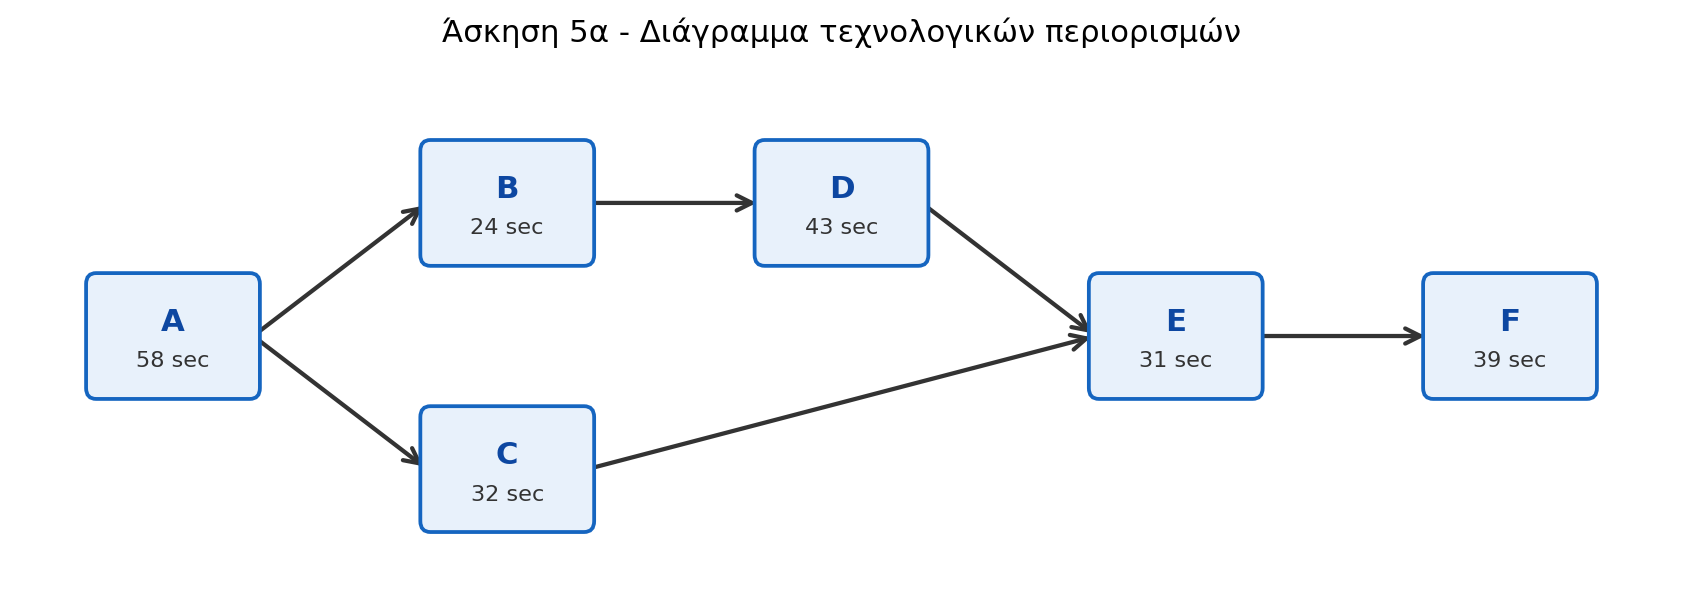
\includegraphics[width=0.95\textwidth]{askisi_5_diagramma_texnologikon_periorismon.png}
\caption{Διάγραμμα τεχνολογικών περιορισμών Άσκησης 5}
\end{figure}

Ερμηνεία: η εργασία E δεν μπορεί να ξεκινήσει αν δεν έχουν ολοκληρωθεί και η C και η D. Επίσης η F είναι η τελευταία εργασία, επειδή απαιτεί πρώτα την ολοκλήρωση της E.

\section{Λύση ερωτήματος β}

\subsection{Τι ζητά το ερώτημα β}

Το ερώτημα β ζητά τον χρονικό κύκλο που επιτρέπει στη γραμμή να παράγει 40 μονάδες ανά ώρα.

Μία ώρα έχει:
\[
3.600 \text{ sec}
\]

Θέλουμε:
\[
40 \text{ μονάδες/ώρα}
\]

Άρα:
\[
C=\frac{3.600}{40}
\]

\[
\boxed{C=90 \text{ sec/μονάδα}}
\]

Ερμηνεία: για να παράγει η γραμμή 40 προϊόντα την ώρα, πρέπει να ολοκληρώνεται ένα προϊόν κάθε 90 δευτερόλεπτα. Επομένως, κανένας σταθμός εργασίας δεν πρέπει να ξεπερνά τα 90 δευτερόλεπτα συνολικής εργασίας.

\section{Λύση ερωτήματος γ}

\subsection{Τι ζητά το ερώτημα γ}

Το ερώτημα γ ζητά τον θεωρητικά ελάχιστο αριθμό σταθμών εργασίας.

Πρώτα υπολογίζουμε το συνολικό περιεχόμενο εργασίας:
\[
\sum t_i=58+24+32+43+31+39
\]

\[
\sum t_i=227 \text{ sec}
\]

Ο χρονικός κύκλος είναι:
\[
C=90 \text{ sec}
\]

Άρα:
\[
N_{\min}=\left\lceil \frac{227}{90} \right\rceil
\]

\[
\frac{227}{90}=2{,}52
\]

Επειδή δεν μπορούμε να έχουμε 2,52 σταθμούς, στρογγυλοποιούμε προς τα πάνω:
\[
\boxed{N_{\min}=3 \text{ σταθμοί}}
\]

Ερμηνεία: θεωρητικά, αν οι εργασίες μπορούν να μοιραστούν κατάλληλα, αρκούν 3 σταθμοί για να επιτευχθεί ο ρυθμός παραγωγής των 40 μονάδων ανά ώρα.

\section{Λύση ερωτήματος δ}

\subsection{Τι ζητά το ερώτημα δ}

Το ερώτημα δ ζητά να κατανείμουμε τις εργασίες σε σταθμούς εργασίας.

Πρέπει να τηρηθούν δύο βασικοί κανόνες:

\begin{itemize}
    \item Ο χρόνος κάθε σταθμού δεν πρέπει να ξεπερνά τον χρονικό κύκλο των 90 sec.
    \item Δεν πρέπει να παραβιάζονται οι τεχνολογικοί περιορισμοί.
\end{itemize}

\subsection{Προτεινόμενη κατανομή}

Μία εφικτή κατανομή είναι:

\begin{table}[H]
\centering
\caption{Κατανομή εργασιών σε σταθμούς}
\begin{tabular}{llcc}
\toprule
\textbf{Σταθμός} & \textbf{Εργασίες} & \textbf{Χρόνος σταθμού} & \textbf{Νεκρός χρόνος} \\
\midrule
1 & A, B & \(58+24=82\) sec & \(90-82=8\) sec \\
2 & C, D & \(32+43=75\) sec & \(90-75=15\) sec \\
3 & E, F & \(31+39=70\) sec & \(90-70=20\) sec \\
\bottomrule
\end{tabular}
\end{table}

\subsection{Γιατί η κατανομή είναι εφικτή}

Ελέγχουμε πρώτα τους χρόνους:

\begin{itemize}
    \item Ο σταθμός 1 έχει 82 sec, άρα \(82 \leq 90\).
    \item Ο σταθμός 2 έχει 75 sec, άρα \(75 \leq 90\).
    \item Ο σταθμός 3 έχει 70 sec, άρα \(70 \leq 90\).
\end{itemize}

Άρα κανένας σταθμός δεν ξεπερνά τον χρονικό κύκλο.

Ελέγχουμε τώρα τις προτεραιότητες:

\begin{itemize}
    \item Η A είναι στον σταθμό 1, πριν από τις B και C.
    \item Η B είναι στον σταθμό 1 και η D στον σταθμό 2, άρα η B προηγείται της D.
    \item Η C είναι στον σταθμό 2 και η E στον σταθμό 3, άρα η C προηγείται της E.
    \item Η D είναι στον σταθμό 2 και η E στον σταθμό 3, άρα η D προηγείται της E.
    \item Η E και η F είναι στον σταθμό 3, με τη σειρά E πριν από F.
\end{itemize}

Επομένως η κατανομή είναι αποδεκτή.

\section{Λύση ερωτήματος ε}

\subsection{Τι ζητά το ερώτημα ε}

Το ερώτημα ε ζητά δύο μέτρα αξιολόγησης της κατανομής:

\begin{itemize}
    \item την αποδοτικότητα,
    \item τον δείκτη ομαλότητας.
\end{itemize}

\subsection{Υπολογισμός αποδοτικότητας}

Ο συνολικός χρόνος εργασιών είναι:
\[
\sum t_i=227 \text{ sec}
\]

Έχουμε:
\[
N=3 \text{ σταθμοί}
\]

και:
\[
C=90 \text{ sec}
\]

Ο συνολικός διαθέσιμος χρόνος των σταθμών ανά κύκλο είναι:
\[
N\cdot C=3\cdot90=270 \text{ sec}
\]

Άρα η αποδοτικότητα είναι:
\[
E=\frac{227}{270}
\]

\[
E=0{,}8407
\]

\[
\boxed{E=84{,}07\%}
\]

Ερμηνεία: το 84,07\% του διαθέσιμου χρόνου των σταθμών χρησιμοποιείται για πραγματική εργασία. Το υπόλοιπο είναι νεκρός χρόνος.

\subsection{Συνολικός νεκρός χρόνος}

Ο συνολικός νεκρός χρόνος είναι:
\[
270-227=43 \text{ sec}
\]

Μπορούμε να τον δούμε και από τον πίνακα:
\[
8+15+20=43 \text{ sec}
\]

\subsection{Υπολογισμός δείκτη ομαλότητας}

Οι χρόνοι των σταθμών είναι:
\[
ST_1=82,\quad ST_2=75,\quad ST_3=70
\]

Ο μεγαλύτερος χρόνος σταθμού είναι:
\[
ST_{\max}=82
\]

Ο δείκτης ομαλότητας είναι:
\[
SI=\sqrt{(ST_{\max}-ST_1)^2+(ST_{\max}-ST_2)^2+(ST_{\max}-ST_3)^2}
\]

Αντικαθιστούμε:
\[
SI=\sqrt{(82-82)^2+(82-75)^2+(82-70)^2}
\]

\[
SI=\sqrt{0^2+7^2+12^2}
\]

\[
SI=\sqrt{193}
\]

\[
\boxed{SI=13{,}89 \text{ sec}}
\]

Ερμηνεία: ο δείκτης ομαλότητας δείχνει ότι οι σταθμοί δεν έχουν ακριβώς τον ίδιο φόρτο, αλλά η κατανομή είναι αρκετά καλή, γιατί όλοι οι σταθμοί είναι κάτω από τα 90 sec και χρησιμοποιούμε τον θεωρητικά ελάχιστο αριθμό σταθμών.

\subsection{Σημείωση για εναλλακτικό ορισμό}

Σε ορισμένες περιπτώσεις ο δείκτης ομαλότητας υπολογίζεται ως απόσταση από τον χρονικό κύκλο \(C=90\) και όχι από τον μεγαλύτερο χρόνο σταθμού. Τότε:
\[
SI_C=\sqrt{(90-82)^2+(90-75)^2+(90-70)^2}
\]

\[
SI_C=\sqrt{8^2+15^2+20^2}
\]

\[
SI_C=26{,}25 \text{ sec}
\]

Στο κύριο αποτέλεσμα χρησιμοποιήθηκε ο συνήθης ορισμός με βάση το \(ST_{\max}\), που δίνει:
\[
SI=13{,}89 \text{ sec}
\]

\section{Τελικό συμπέρασμα Άσκησης 5}

Η Άσκηση 5 δείχνει πώς σχεδιάζουμε και αξιολογούμε μια γραμμή συναρμολόγησης.

Τα βασικά αποτελέσματα είναι:

\begin{itemize}
    \item Ο χρονικός κύκλος που απαιτείται για παραγωγή 40 μονάδων ανά ώρα είναι 90 sec.
    \item Το συνολικό περιεχόμενο εργασίας είναι 227 sec.
    \item Ο θεωρητικά ελάχιστος αριθμός σταθμών είναι 3.
    \item Η προτεινόμενη κατανομή είναι: σταθμός 1 με A και B, σταθμός 2 με C και D, σταθμός 3 με E και F.
    \item Η αποδοτικότητα της γραμμής είναι 84,07\%.
    \item Ο δείκτης ομαλότητας είναι 13,89 sec.
\end{itemize}

Το βασικό διοικητικό συμπέρασμα είναι ότι η γραμμή μπορεί να σχεδιαστεί με 3 σταθμούς, χωρίς να ξεπεραστεί ο χρονικός κύκλος των 90 sec και χωρίς να παραβιαστούν οι τεχνολογικοί περιορισμοί. Η κατανομή έχει κάποιον νεκρό χρόνο, αλλά πετυχαίνει τον ζητούμενο ρυθμό παραγωγής.

\newpage

\section{Άσκηση 6}

\subsection{Η εκφώνηση με απλά λόγια}

Στην Άσκηση 6 έχουμε τη ζήτηση ενός προϊόντος για τους τελευταίους 24 μήνες. Δηλαδή γνωρίζουμε πόσες μονάδες ζητήθηκαν σε κάθε έναν από τους 24 προηγούμενους μήνες.

Το ζητούμενο είναι να χρησιμοποιήσουμε αυτά τα παλαιότερα δεδομένα για να προβλέψουμε τη μελλοντική ζήτηση. Η μέθοδος που ζητά η εκφώνηση είναι η απλή εκθετική εξομάλυνση.

Η άσκηση δεν μας ζητά απλώς να εφαρμόσουμε τη μέθοδο με μία τιμή της παραμέτρου \(\alpha\). Μας δίνει δύο πιθανές τιμές:

\[
\alpha=0{,}1
\]

και:

\[
\alpha=0{,}2
\]

και μας ζητά να διαλέξουμε ποια είναι καλύτερη, συγκρίνοντας την ακρίβεια των προβλέψεων για τους μήνες 13 έως 24.

Με απλά λόγια, το ερώτημα είναι:

\begin{quote}
Αν χρησιμοποιήσουμε την απλή εκθετική εξομάλυνση, ποια τιμή της παραμέτρου \(\alpha\) δίνει πιο ακριβείς προβλέψεις; Και αφού τη διαλέξουμε, ποια είναι η πρόβλεψη για τους μήνες 25 έως 36;
\end{quote}

\subsection{Γιατί συγκρίνουμε στους μήνες 13 έως 24}

Η εκφώνηση μάς λέει να χρησιμοποιήσουμε ως αρχική εκτίμηση στο τέλος του μήνα 11 τη μέση ζήτηση των 11 πρώτων μηνών.

Αυτό σημαίνει ότι πρώτα φτιάχνουμε μια αρχική πρόβλεψη για τον μήνα 12. Στη συνέχεια, χρησιμοποιώντας τη μέθοδο της εκθετικής εξομάλυνσης, μπορούμε να δημιουργήσουμε προβλέψεις για τους επόμενους μήνες.

Η σύγκριση γίνεται στους μήνες 13 έως 24 επειδή για αυτούς τους μήνες έχουμε και πρόβλεψη και πραγματική ζήτηση. Άρα μπορούμε να μετρήσουμε πόσο έξω έπεσε η μέθοδος.

\section{Δεδομένα Άσκησης 6}

\subsection{Αντικατάσταση του x}

Σε όλη την εργασία:
\[
x=211
\]

Οι τιμές που περιέχουν το \(x\) είναι:

\[
280-\frac{x}{4}=280-\frac{211}{4}=227{,}25
\]

Στρογγυλοποιούμε:
\[
227{,}25 \simeq 227
\]

Η δεύτερη τιμή που περιέχει το \(x\) είναι:
\[
145+\frac{x}{2}=145+\frac{211}{2}=250{,}50
\]

Στρογγυλοποίηση:
\[
250{,}50 \simeq 251
\]

Η τρίτη είναι:
\[
150+\frac{x}{5}=150+\frac{211}{5}=192{,}20
\]

Στρογγυλοποίηση:
\[
192{,}20 \simeq 192
\]

Η τέταρτη είναι:
\[
267-\frac{x}{4}=267-\frac{211}{4}=214{,}25
\]

Στρογγυλοποίηση:
\[
214{,}25 \simeq 214
\]

\subsection{Τελική χρονοσειρά ζήτησης}

Μετά τη στρογγυλοποίηση, η ζήτηση των 24 μηνών είναι:

\begin{table}[H]
\centering
\caption{Ζήτηση ανά μήνα μετά τη στρογγυλοποίηση}
\small
\begin{tabular}{rrrrrrrr}
\toprule
\textbf{Μήνας} & 1 & 2 & 3 & 4 & 5 & 6 & 7 \\
\midrule
\textbf{Ζήτηση} & 227 & 250 & 218 & 180 & 192 & 205 & 188 \\
\midrule
\textbf{Μήνας} & 8 & 9 & 10 & 11 & 12 & 13 & 14 \\
\midrule
\textbf{Ζήτηση} & 235 & 190 & 187 & 251 & 275 & 192 & 226 \\
\midrule
\textbf{Μήνας} & 15 & 16 & 17 & 18 & 19 & 20 & 21 \\
\midrule
\textbf{Ζήτηση} & 200 & 173 & 232 & 299 & 173 & 209 & 264 \\
\midrule
\textbf{Μήνας} & 22 & 23 & 24 & & & & \\
\midrule
\textbf{Ζήτηση} & 203 & 214 & 266 & & & & \\
\bottomrule
\end{tabular}
\end{table}

\section{Θεωρητικό υπόβαθρο Άσκησης 6}

\subsection{Τι είναι χρονοσειρά}

Χρονοσειρά είναι μια σειρά παρατηρήσεων που καταγράφονται με τη σειρά του χρόνου. Στην άσκηση, η ζήτηση κάθε μήνα αποτελεί μία παρατήρηση της χρονοσειράς.

Για παράδειγμα:

\[
A_1=227,\quad A_2=250,\quad A_3=218
\]

όπου \(A_t\) σημαίνει πραγματική ζήτηση του μήνα \(t\).

Ο στόχος της πρόβλεψης είναι να χρησιμοποιήσουμε τις προηγούμενες τιμές της χρονοσειράς για να εκτιμήσουμε τις μελλοντικές.

\subsection{Τι είναι απλή εκθετική εξομάλυνση}

Η απλή εκθετική εξομάλυνση είναι μια μέθοδος πρόβλεψης που ενημερώνει την πρόβλεψη κάθε φορά που εμφανίζεται νέο πραγματικό δεδομένο.

Ο τύπος είναι:
\[
F_{t+1}=\alpha A_t+(1-\alpha)F_t
\]

όπου:

\begin{itemize}
    \item \(F_{t+1}\) είναι η πρόβλεψη για τον επόμενο μήνα,
    \item \(A_t\) είναι η πραγματική ζήτηση του τρέχοντος μήνα,
    \item \(F_t\) είναι η πρόβλεψη που είχαμε για τον τρέχοντα μήνα,
    \item \(\alpha\) είναι η σταθερά εξομάλυνσης.
\end{itemize}

Με απλά λόγια, η νέα πρόβλεψη είναι ένας σταθμισμένος μέσος όρος ανάμεσα:

\begin{itemize}
    \item στην πραγματική ζήτηση που μόλις παρατηρήσαμε,
    \item και στην προηγούμενη πρόβλεψη.
\end{itemize}

\subsection{Τι σημαίνει η παράμετρος alpha}

Η παράμετρος \(\alpha\) δείχνει πόσο βάρος δίνουμε στο πιο πρόσφατο πραγματικό δεδομένο.

Αν \(\alpha\) είναι μεγάλο, η πρόβλεψη αντιδρά πιο γρήγορα στις πρόσφατες αλλαγές. Αν \(\alpha\) είναι μικρό, η πρόβλεψη αλλάζει πιο αργά και είναι πιο ομαλή.

Στην άσκηση συγκρίνουμε:

\[
\alpha=0{,}1
\]

και:

\[
\alpha=0{,}2
\]

Το \(\alpha=0{,}2\) δίνει διπλάσιο βάρος στο τελευταίο πραγματικό δεδομένο σε σχέση με το \(\alpha=0{,}1\). Άρα είναι πιο ευαίσθητο στις πρόσφατες μεταβολές.

\subsection{Τι είναι σφάλμα πρόβλεψης}

Το σφάλμα πρόβλεψης είναι η διαφορά ανάμεσα στην πραγματική ζήτηση και στην πρόβλεψη:
\[
e_t=A_t-F_t
\]

Αν το σφάλμα είναι θετικό, η πραγματική ζήτηση ήταν μεγαλύτερη από την πρόβλεψη. Αν είναι αρνητικό, η πρόβλεψη ήταν μεγαλύτερη από την πραγματική ζήτηση.

Για να συγκρίνουμε μεθόδους, δεν αρκεί να κοιτάμε απλώς το άθροισμα των σφαλμάτων, γιατί θετικά και αρνητικά σφάλματα μπορεί να αλληλοαναιρούνται. Για αυτό χρησιμοποιούμε δείκτες ακρίβειας.

\subsection{Δείκτες ακρίβειας}

Στην εργασία χρησιμοποιούμε κυρίως το μέσο απόλυτο σφάλμα, δηλαδή MAD:
\[
MAD=\frac{\sum |A_t-F_t|}{n}
\]

Το MAD δείχνει πόσες μονάδες αποκλίνει κατά μέσο όρο η πρόβλεψη από την πραγματική ζήτηση.

Χρησιμοποιούμε επίσης:

\[
MSE=\frac{\sum (A_t-F_t)^2}{n}
\]

Το MSE δίνει μεγαλύτερη βαρύτητα στα μεγάλα σφάλματα, επειδή τα σφάλματα υψώνονται στο τετράγωνο.

Τέλος, χρησιμοποιούμε και το MAPE:
\[
MAPE=\frac{1}{n}\sum \left|\frac{A_t-F_t}{A_t}\right|\cdot100\%
\]

Το MAPE δείχνει το μέσο ποσοστιαίο σφάλμα.

Σε όλους αυτούς τους δείκτες, μικρότερη τιμή σημαίνει καλύτερη πρόβλεψη.

\section{Αρχική πρόβλεψη}

Η εκφώνηση λέει ότι η αρχική εκτίμηση στο τέλος του μήνα 11 είναι η μέση ζήτηση των 11 πρώτων μηνών.

Οι 11 πρώτοι μήνες είναι:
\[
227,\ 250,\ 218,\ 180,\ 192,\ 205,\ 188,\ 235,\ 190,\ 187,\ 251
\]

Το άθροισμά τους είναι:
\[
2.323
\]

Άρα η αρχική εκτίμηση είναι:
\[
F_{12}=\frac{2.323}{11}
\]

\[
F_{12}=211{,}18
\]

Αυτό σημαίνει ότι, πριν δούμε τη ζήτηση του μήνα 12, η αρχική μας πρόβλεψη για τον μήνα 12 είναι 211,18 μονάδες.

\section{Υπολογισμοί με alpha = 0,1}

\subsection{Πώς ενημερώνεται η πρόβλεψη}

Για \(\alpha=0{,}1\), ο τύπος γίνεται:
\[
F_{t+1}=0{,}1A_t+0{,}9F_t
\]

Για παράδειγμα, η πρόβλεψη για τον μήνα 13 υπολογίζεται χρησιμοποιώντας την πραγματική ζήτηση του μήνα 12 και την πρόβλεψη του μήνα 12:
\[
F_{13}=0{,}1A_{12}+0{,}9F_{12}
\]

Ξέρουμε ότι:
\[
A_{12}=275
\]

και:
\[
F_{12}=211{,}18
\]

Άρα:
\[
F_{13}=0{,}1\cdot275+0{,}9\cdot211{,}18
\]

\[
F_{13}=27{,}50+190{,}06=217{,}56
\]

Με τον ίδιο τρόπο συνεχίζουμε για τους επόμενους μήνες.

\subsection{Πίνακας προβλέψεων και σφαλμάτων για alpha = 0,1}

\begin{table}[H]
\centering
\caption{Προβλέψεις και σφάλματα για \(\alpha=0{,}1\)}
\small
\begin{tabular}{rrrrr}
\toprule
\textbf{Μήνας} & \textbf{Πραγματική ζήτηση} & \textbf{Πρόβλεψη} & \textbf{Σφάλμα} & \textbf{Απόλυτο σφάλμα} \\
\midrule
13 & 192 & 217,56 & -25,56 & 25,56 \\
14 & 226 & 215,01 & 10,99 & 10,99 \\
15 & 200 & 216,11 & -16,11 & 16,11 \\
16 & 173 & 214,50 & -41,50 & 41,50 \\
17 & 232 & 210,35 & 21,65 & 21,65 \\
18 & 299 & 212,51 & 86,49 & 86,49 \\
19 & 173 & 221,16 & -48,16 & 48,16 \\
20 & 209 & 216,34 & -7,34 & 7,34 \\
21 & 264 & 215,61 & 48,39 & 48,39 \\
22 & 203 & 220,45 & -17,45 & 17,45 \\
23 & 214 & 218,70 & -4,70 & 4,70 \\
24 & 266 & 218,23 & 47,77 & 47,77 \\
\bottomrule
\end{tabular}
\end{table}

Από αυτά τα σφάλματα προκύπτουν:
\[
MAD=31{,}34
\]
\[
MSE=1.502{,}33
\]
\[
MAPE=13{,}91\%
\]

\section{Υπολογισμοί με alpha = 0,2}

Για \(\alpha=0{,}2\), ο τύπος γίνεται:
\[
F_{t+1}=0{,}2A_t+0{,}8F_t
\]

Η τιμή \(\alpha=0{,}2\) κάνει την πρόβλεψη να αντιδρά λίγο περισσότερο στις πρόσφατες πραγματικές τιμές.

Για παράδειγμα, η πρόβλεψη για τον μήνα 13 είναι:
\[
F_{13}=0{,}2A_{12}+0{,}8F_{12}
\]

\[
F_{13}=0{,}2\cdot275+0{,}8\cdot211{,}18
\]

\[
F_{13}=55+168{,}95=223{,}95
\]

Με την ίδια διαδικασία υπολογίζονται οι προβλέψεις για τους μήνες 13 έως 24 και μετά τα αντίστοιχα σφάλματα.

Οι δείκτες ακρίβειας που προκύπτουν είναι:
\[
MAD=33{,}63
\]
\[
MSE=1.642{,}75
\]
\[
MAPE=15{,}12\%
\]

\section{Σύγκριση των δύο τιμών alpha}

Συγκεντρώνουμε τα αποτελέσματα:

\begin{table}[H]
\centering
\caption{Σύγκριση ακρίβειας για \(\alpha=0{,}1\) και \(\alpha=0{,}2\)}
\begin{tabular}{lccc}
\toprule
\(\boldsymbol{\alpha}\) & \textbf{MAD} & \textbf{MSE} & \textbf{MAPE} \\
\midrule
0,1 & 31,34 & 1.502,33 & 13,91\% \\
0,2 & 33,63 & 1.642,75 & 15,12\% \\
\bottomrule
\end{tabular}
\end{table}

Και στους τρεις δείκτες, η τιμή \(\alpha=0{,}1\) δίνει μικρότερο σφάλμα.

Άρα επιλέγουμε:
\[
\boxed{\alpha=0{,}1}
\]

Ερμηνεία: για τα συγκεκριμένα δεδομένα, η πιο ήπια εξομάλυνση, δηλαδή το \(\alpha=0{,}1\), αποδίδει καλύτερα. Αυτό σημαίνει ότι δεν συμφέρει να αντιδρά η πρόβλεψη πολύ έντονα στις πρόσφατες μεταβολές της ζήτησης.

\section{Πρόβλεψη για τους μήνες 25 έως 36}

\subsection{Υπολογισμός πρόβλεψης για τον μήνα 25}

Αφού επιλέξαμε:
\[
\alpha=0{,}1
\]

υπολογίζουμε την πρόβλεψη για τον μήνα 25 χρησιμοποιώντας την πραγματική ζήτηση του μήνα 24 και την πρόβλεψη του μήνα 24.

Ξέρουμε:
\[
A_{24}=266
\]

και:
\[
F_{24}=218{,}23
\]

Άρα:
\[
F_{25}=0{,}1A_{24}+0{,}9F_{24}
\]

\[
F_{25}=0{,}1\cdot266+0{,}9\cdot218{,}23
\]

\[
F_{25}=26{,}60+196{,}41
\]

\[
\boxed{F_{25}=223{,}01}
\]

\subsection{Γιατί οι προβλέψεις 25 έως 36 είναι ίδιες}

Η απλή εκθετική εξομάλυνση δεν περιλαμβάνει τάση ή εποχικότητα. Αυτό σημαίνει ότι, αν δεν έχουμε νέα πραγματικά δεδομένα μετά τον μήνα 24, η καλύτερη πρόβλεψη για όλους τους επόμενους μήνες παραμένει ίδια με την πρόβλεψη του επόμενου μήνα.

Άρα:
\[
F_{25}=F_{26}=\cdots=F_{36}=223{,}01
\]

Στρογγυλοποιημένα:
\[
\boxed{F_{25}=F_{26}=\cdots=F_{36}=223 \text{ μονάδες}}
\]

\begin{table}[H]
\centering
\caption{Πρόβλεψη ζήτησης για τους μήνες 25 έως 36}
\begin{tabular}{cc}
\toprule
\textbf{Μήνας} & \textbf{Πρόβλεψη} \\
\midrule
25 & 223,01 \\
26 & 223,01 \\
27 & 223,01 \\
28 & 223,01 \\
29 & 223,01 \\
30 & 223,01 \\
31 & 223,01 \\
32 & 223,01 \\
33 & 223,01 \\
34 & 223,01 \\
35 & 223,01 \\
36 & 223,01 \\
\bottomrule
\end{tabular}
\end{table}

\section{Γράφημα πραγματικής ζήτησης και πρόβλεψης}

Στο παρακάτω γράφημα φαίνονται μαζί η πραγματική ζήτηση και η πρόβλεψη που προέκυψε με την επιλεγμένη τιμή \(\alpha=0{,}1\).

Η μπλε καμπύλη δείχνει την πραγματική ζήτηση για τους μήνες 1 έως 24, δηλαδή τα δεδομένα που μας δίνει η εκφώνηση. Η κόκκινη διακεκομμένη καμπύλη δείχνει την πρόβλεψη της απλής εκθετικής εξομάλυνσης. Η πρόβλεψη ξεκινά από τον μήνα 12, επειδή εκεί έχουμε την αρχική εκτίμηση \(F_{12}=211{,}18\).

Μετά τον μήνα 24, δεν υπάρχουν νέα πραγματικά δεδομένα. Για αυτό η κόκκινη καμπύλη γίνεται οριζόντια στους μήνες 25 έως 36, στην τιμή:
\[
223{,}01
\]

Αυτό ακριβώς εκφράζει η βασική ιδέα της απλής εκθετικής εξομάλυνσης: χωρίς νέα παρατήρηση, η μελλοντική πρόβλεψη παραμένει ίδια.

\begin{figure}[H]
\centering
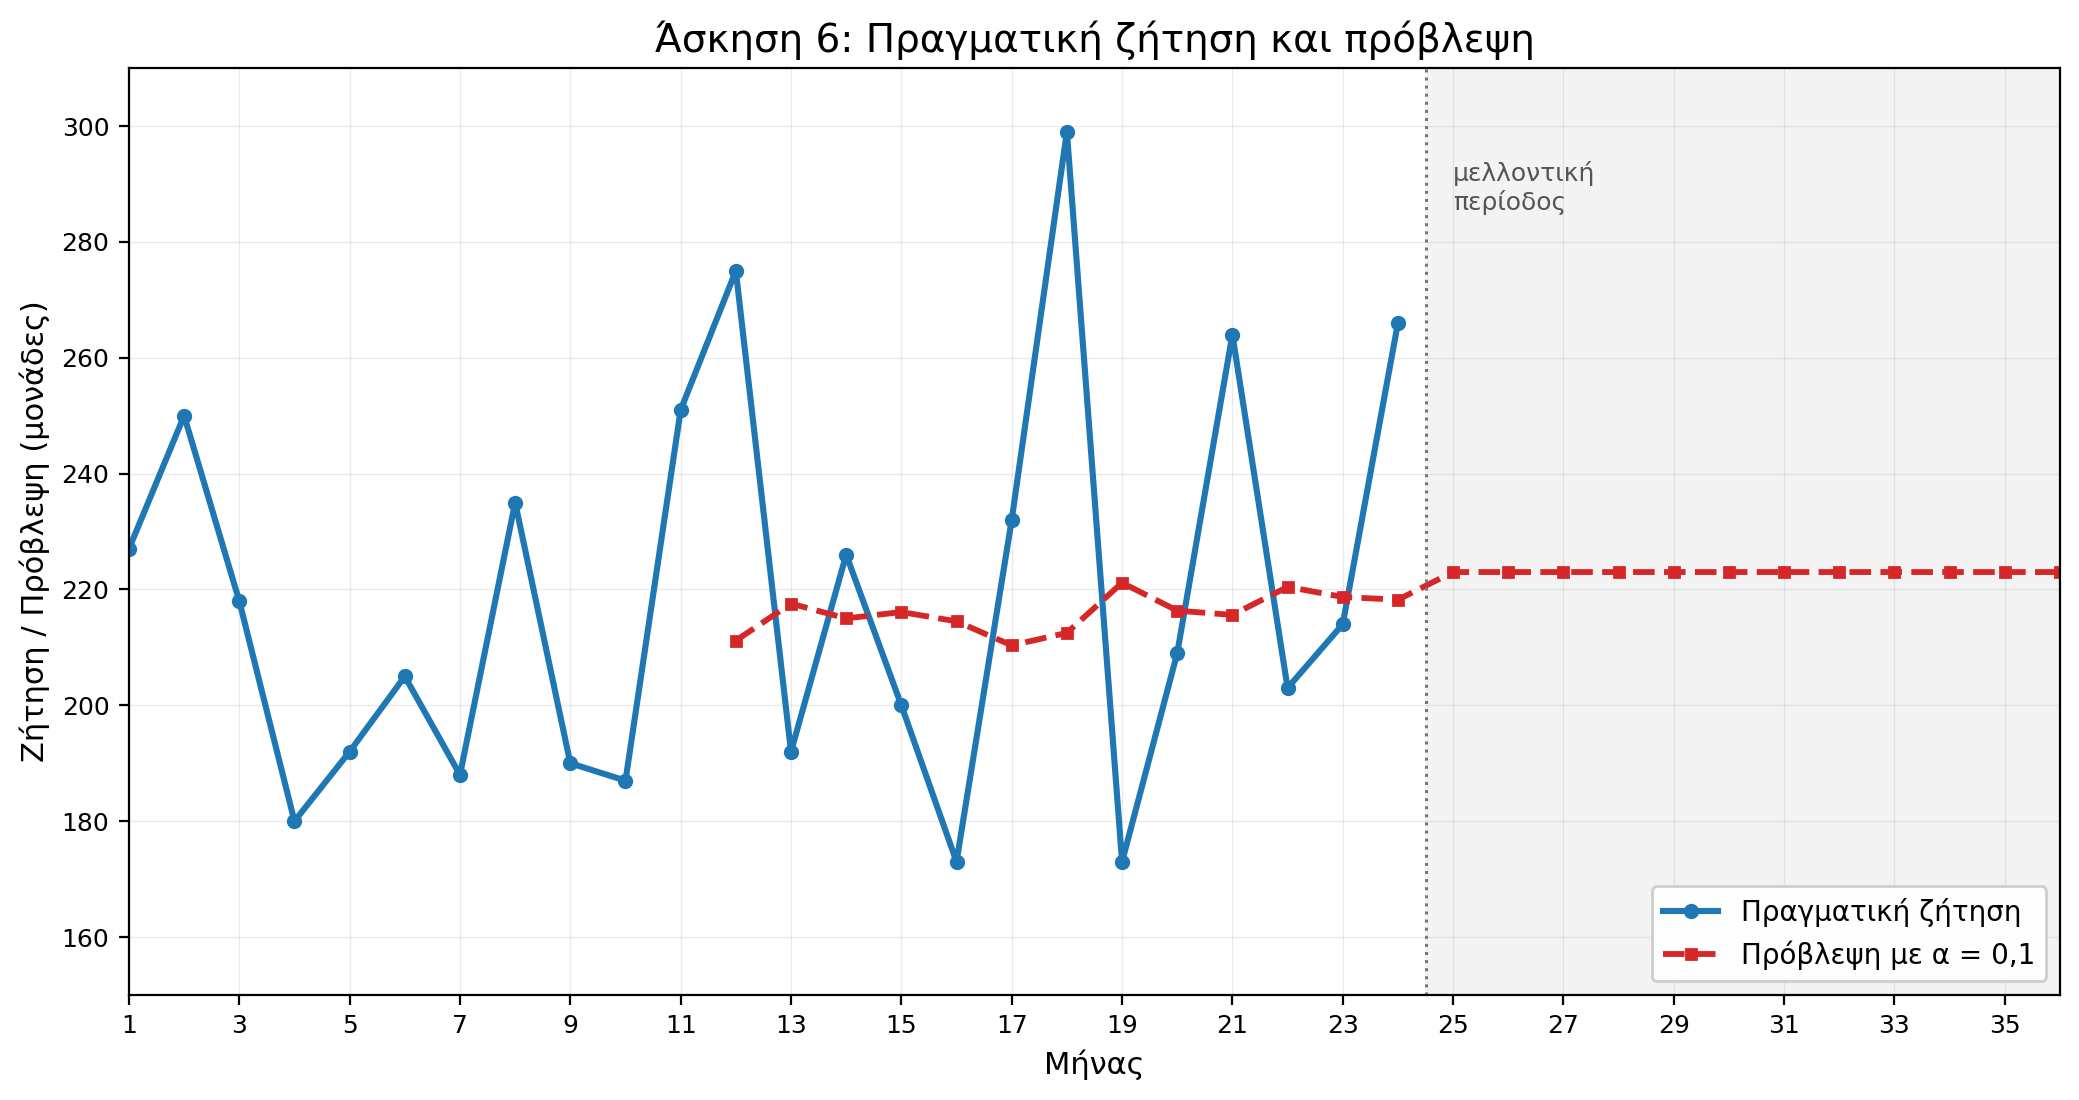
\includegraphics[width=0.96\textwidth]{askisi_6_grafima_zitisis_provlepsis.png}
\caption{Πραγματική ζήτηση και πρόβλεψη με απλή εκθετική εξομάλυνση για \(\alpha=0{,}1\)}
\end{figure}

Για σύγκριση, στο επόμενο γράφημα φαίνεται η αντίστοιχη πρόβλεψη αν χρησιμοποιούσαμε \(\alpha=0{,}2\).

Επειδή το \(\alpha=0{,}2\) δίνει μεγαλύτερο βάρος στην πιο πρόσφατη πραγματική ζήτηση, η πράσινη καμπύλη κινείται λίγο πιο έντονα από την κόκκινη καμπύλη του προηγούμενου γραφήματος. Δηλαδή αντιδρά περισσότερο στις αυξομειώσεις των τελευταίων μηνών.

Αν επιλέγαμε \(\alpha=0{,}2\), η πρόβλεψη για τον μήνα 25 θα ήταν:
\[
F_{25}^{(\alpha=0{,}2)}=229{,}04
\]

και, όπως πριν, επειδή δεν υπάρχουν νέα πραγματικά δεδομένα μετά τον μήνα 24, η πρόβλεψη για τους μήνες 25 έως 36 θα έμενε σταθερή σε αυτή την τιμή. Παρόλα αυτά, η τιμή \(\alpha=0{,}2\) δεν επιλέχθηκε τελικά, επειδή είχε μεγαλύτερα σφάλματα από την τιμή \(\alpha=0{,}1\).

\begin{figure}[H]
\centering
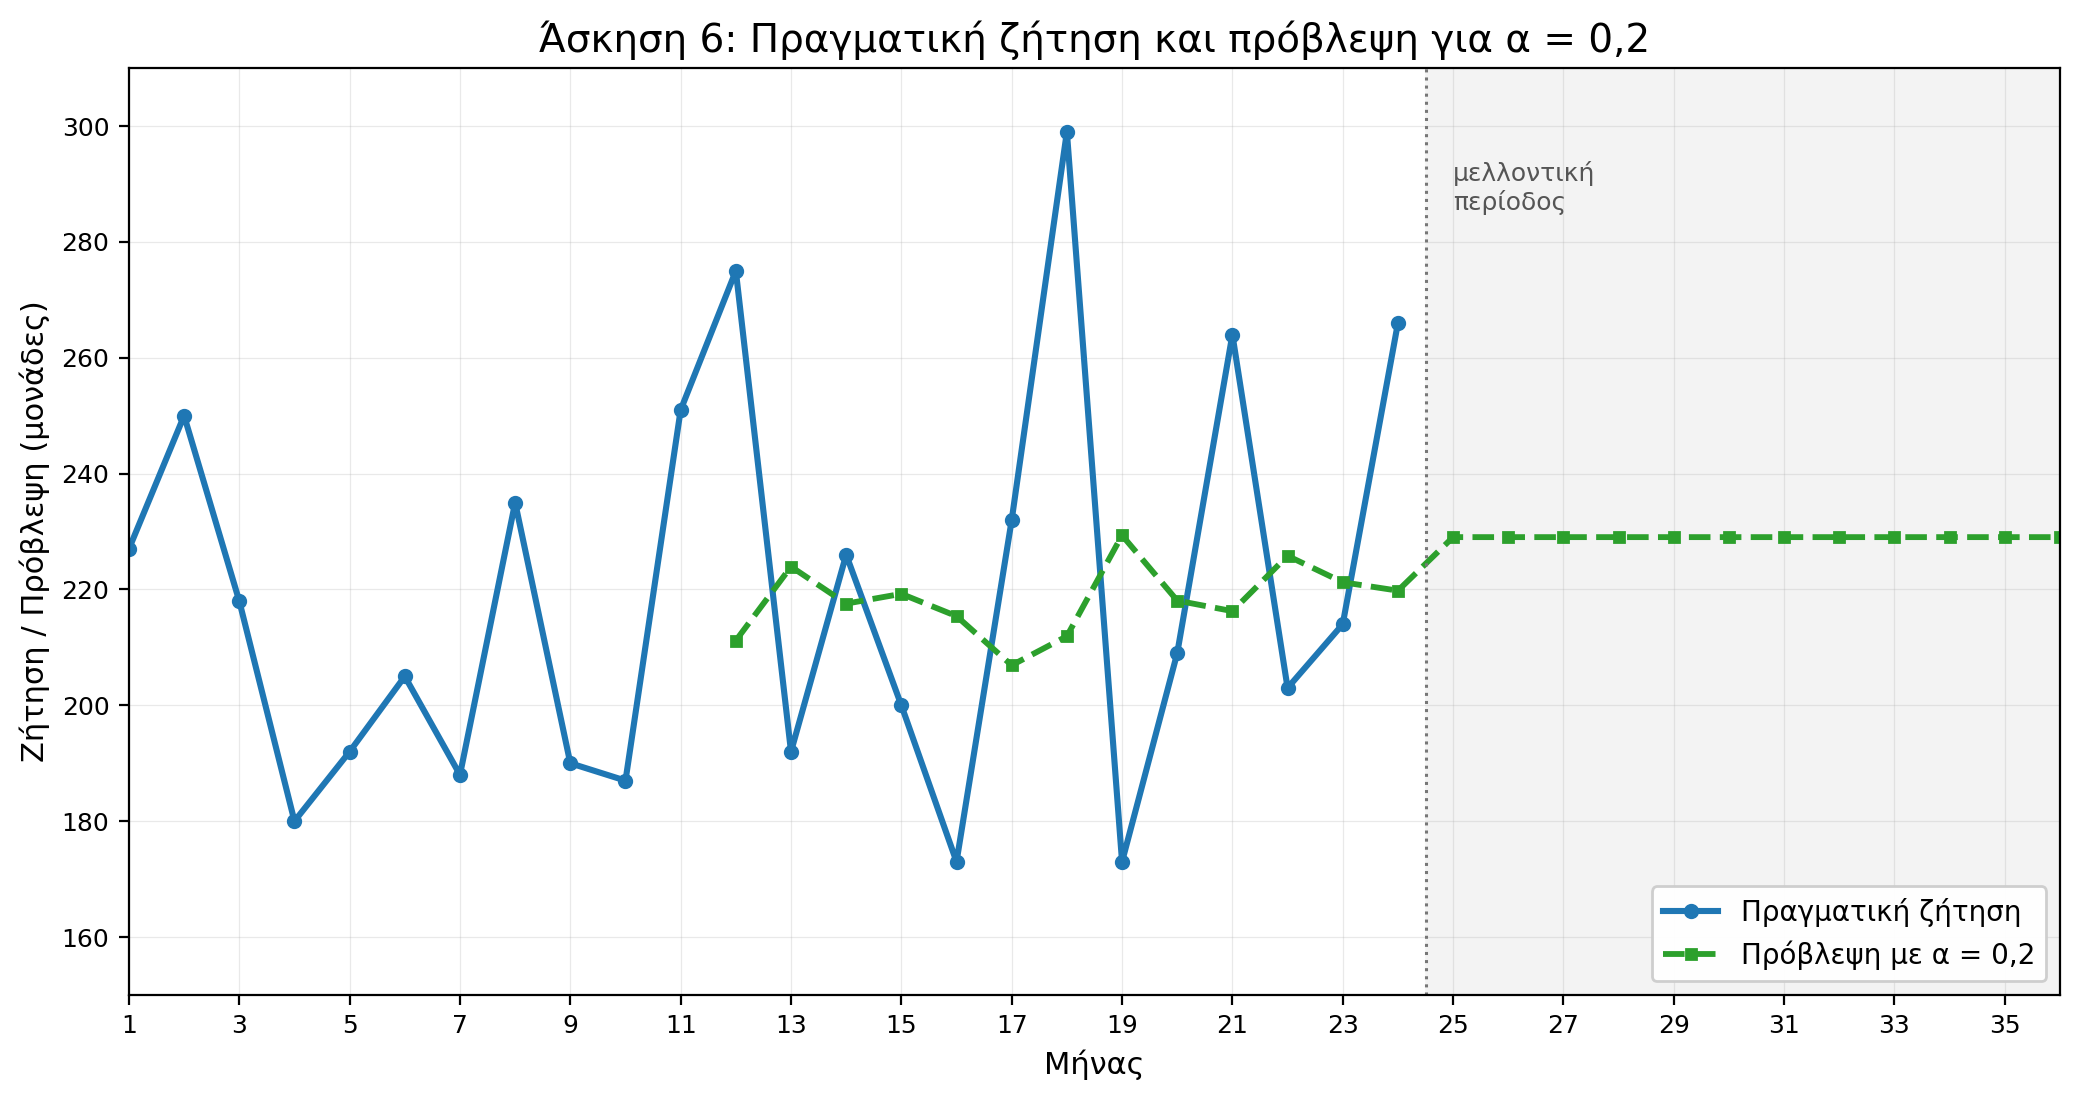
\includegraphics[width=0.96\textwidth]{askisi_6_grafima_zitisis_provlepsis_alpha_02.png}
\caption{Πραγματική ζήτηση και πρόβλεψη με απλή εκθετική εξομάλυνση για \(\alpha=0{,}2\)}
\end{figure}

\section{Τελικό συμπέρασμα Άσκησης 6}

Στην Άσκηση 6 χρησιμοποιήθηκε η μέθοδος της απλής εκθετικής εξομάλυνσης για την πρόβλεψη της μελλοντικής ζήτησης.

Η αρχική εκτίμηση ήταν:
\[
F_{12}=211{,}18
\]

Στη συνέχεια συγκρίθηκαν δύο τιμές της σταθεράς εξομάλυνσης:

\[
\alpha=0{,}1
\]

και:

\[
\alpha=0{,}2
\]

Η τιμή \(\alpha=0{,}1\) είχε μικρότερα σφάλματα:

\[
MAD=31{,}34,\quad MSE=1.502{,}33,\quad MAPE=13{,}91\%
\]

Άρα επιλέχθηκε:
\[
\boxed{\alpha=0{,}1}
\]

Η τελική πρόβλεψη για τους μήνες 25 έως 36 είναι:
\[
\boxed{223{,}01 \text{ μονάδες ανά μήνα}}
\]

ή, στρογγυλοποιημένα:
\[
\boxed{223 \text{ μονάδες ανά μήνα}}
\]

Το διοικητικό συμπέρασμα είναι ότι, με βάση τα διαθέσιμα δεδομένα, η ζήτηση για τους επόμενους 12 μήνες εκτιμάται περίπου στις 223 μονάδες ανά μήνα, εφόσον δεν εισάγονται νέα πραγματικά δεδομένα και χρησιμοποιείται απλή εκθετική εξομάλυνση χωρίς τάση ή εποχικότητα.

\newpage

\section{Άσκηση 7}

\subsection{Η εκφώνηση με απλά λόγια}

Στην Άσκηση 7 ασχολούμαστε με τη διαχείριση αποθεμάτων. Η επιχείρηση έχει ένα προϊόν με σταθερή ζήτηση και χρησιμοποιεί το σύστημα EOQ, δηλαδή το σύστημα οικονομικής ποσότητας παραγγελίας.

Η βασική ιδέα είναι η εξής:

\begin{quote}
Η επιχείρηση πρέπει να αποφασίζει πότε θα δίνει παραγγελία και πόσο θα παραγγέλνει, ώστε να καλύπτει τη ζήτηση χωρίς να κρατά υπερβολικά μεγάλο απόθεμα.
\end{quote}

Η εκφώνηση μάς δίνει:

\begin{itemize}
    \item τη ζήτηση ανά εβδομάδα,
    \item τον χρόνο που χρειάζεται για να φτάσει μια παραγγελία,
    \item το κόστος κάθε παραγγελίας,
    \item και τη βέλτιστη ποσότητα παραγγελίας που ήδη εφαρμόζεται.
\end{itemize}

Ζητά να υπολογίσουμε:

\begin{enumerate}
    \item τη στάθμη παραγγελίας,
    \item το μέσο απόθεμα,
    \item τον χρόνο μεταξύ παραγγελιών,
    \item την κυκλοφοριακή ταχύτητα αποθεμάτων,
    \item τη διάρκεια των αποθεμάτων,
    \item το ετήσιο κόστος παραγγελιών και διατήρησης,
    \item και το κόστος διατήρησης μιας μονάδας αποθέματος για ένα έτος.
\end{enumerate}

\section{Δεδομένα Άσκησης 7}

Σε όλη την εργασία:
\[
x=211
\]

Η ζήτηση είναι:
\[
80 \text{ μονάδες/εβδομάδα}
\]

Επειδή το έτος έχει 52 εβδομάδες, η ετήσια ζήτηση είναι:
\[
D=80\cdot52
\]

\[
D=4.160 \text{ μονάδες/έτος}
\]

Ο χρόνος ικανοποίησης παραγγελίας είναι:
\[
L=1 \text{ εβδομάδα}
\]

Το σταθερό κόστος κάθε παραγγελίας είναι:
\[
S=50+x=50+211=261 \text{ €/παραγγελία}
\]

Η βέλτιστη ποσότητα παραγγελίας είναι:
\[
Q=100+x=100+211=311 \text{ μονάδες}
\]

Συνοπτικά:

\begin{table}[H]
\centering
\caption{Δεδομένα συστήματος EOQ}
\begin{tabular}{lc}
\toprule
\textbf{Μέγεθος} & \textbf{Τιμή} \\
\midrule
Εβδομαδιαία ζήτηση \(d\) & 80 μονάδες/εβδομάδα \\
Ετήσια ζήτηση \(D\) & 4.160 μονάδες/έτος \\
Lead time \(L\) & 1 εβδομάδα \\
Κόστος παραγγελίας \(S\) & 261 €/παραγγελία \\
Ποσότητα παραγγελίας \(Q\) & 311 μονάδες \\
\bottomrule
\end{tabular}
\end{table}

\section{Θεωρητικό υπόβαθρο Άσκησης 7}

\subsection{Τι είναι απόθεμα}

Απόθεμα είναι η ποσότητα προϊόντων που κρατά μια επιχείρηση διαθέσιμη, ώστε να μπορεί να καλύπτει τη ζήτηση των πελατών.

Αν το απόθεμα είναι πολύ μικρό, υπάρχει κίνδυνος να μην μπορεί η επιχείρηση να εξυπηρετήσει τη ζήτηση. Αν το απόθεμα είναι πολύ μεγάλο, τότε δεσμεύονται χρήματα, χώρος και πόροι.

Άρα η διαχείριση αποθεμάτων προσπαθεί να βρει μια ισορροπία.

\subsection{Τι είναι το σύστημα EOQ}

EOQ σημαίνει Economic Order Quantity, δηλαδή οικονομική ποσότητα παραγγελίας.

Το μοντέλο EOQ απαντά στο ερώτημα:

\begin{quote}
Πόσες μονάδες πρέπει να παραγγέλνουμε κάθε φορά, ώστε το συνολικό κόστος παραγγελιών και διατήρησης αποθέματος να είναι όσο γίνεται μικρότερο;
\end{quote}

Στην άσκηση δεν χρειάζεται να βρούμε την EOQ από την αρχή, επειδή μας δίνεται ότι η βέλτιστη ποσότητα παραγγελίας που εφαρμόζεται είναι:
\[
Q=311
\]

Όμως χρησιμοποιούμε τη λογική του EOQ για να υπολογίσουμε τα κόστη.

\subsection{Τι είναι κόστος παραγγελίας}

Κόστος παραγγελίας είναι το σταθερό κόστος που δημιουργείται κάθε φορά που γίνεται μία παραγγελία, ανεξάρτητα από την ποσότητα που παραγγέλνουμε.

Περιλαμβάνει, για παράδειγμα:

\begin{itemize}
    \item διοικητικό κόστος έκδοσης παραγγελίας,
    \item κόστος επικοινωνίας με προμηθευτή,
    \item κόστος παραλαβής,
    \item κόστος ελέγχου παραγγελίας.
\end{itemize}

Στην άσκηση:
\[
S=261 \text{ €/παραγγελία}
\]

\subsection{Τι είναι κόστος διατήρησης αποθέματος}

Κόστος διατήρησης είναι το κόστος που έχει η επιχείρηση επειδή κρατά απόθεμα.

Μπορεί να περιλαμβάνει:

\begin{itemize}
    \item κόστος αποθήκευσης,
    \item κόστος κεφαλαίου που δεσμεύεται σε απόθεμα,
    \item ασφάλιστρα,
    \item φθορές ή απαξίωση προϊόντων.
\end{itemize}

Στο EOQ, το κόστος διατήρησης ανά μονάδα ανά έτος συμβολίζεται συνήθως με \(H\).

\subsection{Τι είναι στάθμη παραγγελίας}

Η στάθμη παραγγελίας είναι το επίπεδο αποθέματος στο οποίο πρέπει να δοθεί νέα παραγγελία.

Δεν περιμένουμε να μηδενιστεί το απόθεμα για να παραγγείλουμε. Αν το κάναμε, μέχρι να φτάσει η νέα παραγγελία, η επιχείρηση θα έμενε χωρίς προϊόν.

Γι' αυτό δίνουμε παραγγελία νωρίτερα, όταν το απόθεμα πέσει σε ένα συγκεκριμένο επίπεδο.

Χωρίς απόθεμα ασφαλείας, ο τύπος είναι:
\[
ROP=d\cdot L
\]

όπου:

\begin{itemize}
    \item \(ROP\) είναι η στάθμη παραγγελίας,
    \item \(d\) είναι η ζήτηση ανά χρονική περίοδο,
    \item \(L\) είναι ο χρόνος ικανοποίησης παραγγελίας.
\end{itemize}

\subsection{Τι είναι μέσο απόθεμα}

Στο βασικό μοντέλο EOQ, το απόθεμα ξεκινά από \(Q\) όταν παραλαμβάνεται η παραγγελία και μειώνεται σταδιακά μέχρι να φτάσει περίπου στο μηδέν πριν από την επόμενη παραλαβή.

Άρα το μέσο απόθεμα είναι:
\[
I_{\text{μέσο}}=\frac{Q}{2}
\]

\subsection{Τι είναι κυκλοφοριακή ταχύτητα αποθεμάτων}

Η κυκλοφοριακή ταχύτητα αποθεμάτων δείχνει πόσες φορές μέσα στο έτος ανανεώνεται το μέσο απόθεμα.

Ο τύπος είναι:
\[
\text{Κυκλοφοριακή ταχύτητα}=
\frac{\text{Ετήσια ζήτηση}}{\text{Μέσο απόθεμα}}
\]

Μεγάλη κυκλοφοριακή ταχύτητα σημαίνει ότι το απόθεμα ανανεώνεται συχνά.

\subsection{Τι είναι διάρκεια αποθεμάτων}

Η διάρκεια αποθεμάτων δείχνει για πόσο χρόνο επαρκεί το μέσο απόθεμα, αν συνεχιστεί η ζήτηση με τον ίδιο ρυθμό.

Σε εβδομάδες:
\[
\text{Διάρκεια αποθεμάτων}=
\frac{\text{Μέσο απόθεμα}}{\text{Εβδομαδιαία ζήτηση}}
\]

\section{Λύση ερωτήματος α}

\subsection{Τι ζητά το ερώτημα α}

Το ερώτημα α ζητά τη στάθμη παραγγελίας, δηλαδή σε ποιο επίπεδο αποθέματος πρέπει να δοθεί νέα παραγγελία.

Η ζήτηση είναι:
\[
d=80 \text{ μονάδες/εβδομάδα}
\]

Ο χρόνος ικανοποίησης παραγγελίας είναι:
\[
L=1 \text{ εβδομάδα}
\]

Άρα:
\[
ROP=d\cdot L
\]

\[
ROP=80\cdot1=80
\]

\[
\boxed{ROP=80 \text{ μονάδες}}
\]

Ερμηνεία: όταν το απόθεμα πέσει στις 80 μονάδες, πρέπει να δοθεί νέα παραγγελία. Οι 80 μονάδες επαρκούν για να καλυφθεί η ζήτηση της μίας εβδομάδας μέχρι να φτάσει η νέα παραγγελία.

\section{Λύση ερωτήματος β}

\subsection{Μέσο απόθεμα}

Η ποσότητα παραγγελίας είναι:
\[
Q=311
\]

Στο EOQ, το μέσο απόθεμα είναι:
\[
I_{\text{μέσο}}=\frac{Q}{2}
\]

Άρα:
\[
I_{\text{μέσο}}=\frac{311}{2}=155{,}5
\]

\[
\boxed{I_{\text{μέσο}}=155{,}5 \text{ μονάδες}}
\]

\subsection{Χρόνος μεταξύ διαδοχικών παραγγελιών}

Ο χρόνος μεταξύ δύο παραγγελιών δείχνει κάθε πόσες εβδομάδες δίνεται νέα παραγγελία.

Αν κάθε φορά παραγγέλνουμε 311 μονάδες και η ζήτηση είναι 80 μονάδες ανά εβδομάδα, τότε:
\[
T=\frac{Q}{d}
\]

\[
T=\frac{311}{80}=3{,}8875
\]

\[
\boxed{T=3{,}89 \text{ εβδομάδες}}
\]

Ερμηνεία: περίπου κάθε 3,89 εβδομάδες η επιχείρηση δίνει νέα παραγγελία.

\subsection{Αριθμός παραγγελιών ανά έτος}

Ο αριθμός παραγγελιών ανά έτος είναι:
\[
N=\frac{D}{Q}
\]

\[
N=\frac{4.160}{311}=13{,}38
\]

\[
\boxed{N=13{,}38 \text{ παραγγελίες/έτος}}
\]

Ερμηνεία: η επιχείρηση δίνει περίπου 13 με 14 παραγγελίες τον χρόνο.

\subsection{Κυκλοφοριακή ταχύτητα αποθεμάτων}

Η κυκλοφοριακή ταχύτητα είναι:
\[
\frac{D}{I_{\text{μέσο}}}
\]

\[
\frac{4.160}{155{,}5}=26{,}75
\]

\[
\boxed{26{,}75 \text{ φορές/έτος}}
\]

Ερμηνεία: το μέσο απόθεμα ανανεώνεται περίπου 26,75 φορές μέσα στο έτος.

\subsection{Διάρκεια αποθεμάτων}

Η διάρκεια αποθεμάτων σε εβδομάδες είναι:
\[
\frac{I_{\text{μέσο}}}{d}
\]

\[
\frac{155{,}5}{80}=1{,}94375
\]

\[
\boxed{1{,}94 \text{ εβδομάδες}}
\]

Ερμηνεία: το μέσο απόθεμα επαρκεί για περίπου 1,94 εβδομάδες ζήτησης.

\section{Λύση ερωτήματος γ}

\subsection{Τι ζητά το ερώτημα γ}

Το ερώτημα γ ζητά το μέσο ετήσιο συνολικό κόστος παραγγελιών και διατήρησης αποθεμάτων.

Το συνολικό κόστος αποτελείται από δύο μέρη:

\[
TC=\text{Ετήσιο κόστος παραγγελιών}+\text{Ετήσιο κόστος διατήρησης}
\]

Ο τύπος αυτός λέει κάτι απλό: για να διαχειριστεί η επιχείρηση το απόθεμά της, πληρώνει κόστος για δύο διαφορετικούς λόγους.

Πρώτον, πληρώνει κάθε φορά που δίνει παραγγελία. Αυτό είναι το κόστος παραγγελιών.

Δεύτερον, πληρώνει επειδή κρατά προϊόντα σε απόθεμα. Αυτό είναι το κόστος διατήρησης αποθεμάτων.

Άρα το ετήσιο συνολικό κόστος είναι το άθροισμα αυτών των δύο κατηγοριών κόστους.

\subsection{Ετήσιο κόστος παραγγελιών}

Το ετήσιο κόστος παραγγελιών είναι:
\[
\text{Κόστος παραγγελιών}=\frac{D}{Q}\cdot S
\]

Ας εξηγήσουμε τον τύπο κομμάτι κομμάτι.

Το \(D\) είναι η συνολική ετήσια ζήτηση. Στην άσκηση:
\[
D=4.160 \text{ μονάδες/έτος}
\]

Το \(Q\) είναι η ποσότητα που παραγγέλνουμε κάθε φορά. Στην άσκηση:
\[
Q=311 \text{ μονάδες/παραγγελία}
\]

Άρα το κλάσμα:
\[
\frac{D}{Q}
\]

δείχνει πόσες παραγγελίες θα γίνουν μέσα στο έτος. Δηλαδή:
\[
\frac{4.160}{311}=13{,}38
\]

Αυτό σημαίνει ότι η επιχείρηση κάνει περίπου 13,38 παραγγελίες τον χρόνο.

Το \(S\) είναι το σταθερό κόστος κάθε παραγγελίας. Στην άσκηση:
\[
S=261 \text{ €/παραγγελία}
\]

Άρα:
\[
\frac{D}{Q}\cdot S
\]

σημαίνει:

\begin{quote}
αριθμός παραγγελιών ανά έτος \(\times\) κόστος κάθε παραγγελίας.
\end{quote}

Έτσι βρίσκουμε πόσα ευρώ πληρώνει συνολικά η επιχείρηση μέσα στο έτος μόνο για τη διαδικασία των παραγγελιών.

Αντικαθιστούμε:
\[
\frac{4.160}{311}\cdot261
\]

\[
\boxed{\text{Κόστος παραγγελιών}=3.491{,}19 \text{ €}}
\]

\subsection{Ετήσιο κόστος διατήρησης}

Εδώ θέλει λίγη προσοχή. Γενικά, το ετήσιο κόστος παραγγελιών δεν είναι πάντα ίσο με το ετήσιο κόστος διατήρησης. Η ισότητα αυτή ισχύει ειδικά στο άριστο σημείο του μοντέλου EOQ.

Στην εκφώνηση όμως δίνεται ότι η ποσότητα παραγγελίας που εφαρμόζεται είναι η βέλτιστη ποσότητα παραγγελίας, δηλαδή:
\[
Q=EOQ=311
\]

Άρα βρισκόμαστε στο άριστο σημείο του EOQ.

Στο μοντέλο EOQ ισχύουν τα εξής:

\[
\text{Ετήσιο κόστος παραγγελιών}=\frac{D}{Q}\cdot S
\]

Αυτός είναι ο τύπος που εξηγήσαμε πριν: όσο μικρότερη είναι η ποσότητα παραγγελίας \(Q\), τόσο περισσότερες παραγγελίες χρειάζονται μέσα στο έτος, άρα αυξάνεται το κόστος παραγγελιών.

και:

\[
\text{Ετήσιο κόστος διατήρησης}=\frac{Q}{2}\cdot H
\]

Εδώ το \(\frac{Q}{2}\) είναι το μέσο απόθεμα.

Γιατί είναι \(Q/2\); Στο απλό μοντέλο EOQ, όταν φτάνει μια παραγγελία, το απόθεμα ανεβαίνει περίπου στο \(Q\). Μετά, καθώς υπάρχει ζήτηση, το απόθεμα μειώνεται σταδιακά μέχρι να φτάσει κοντά στο 0, πριν έρθει η επόμενη παραγγελία.

Άρα το απόθεμα κινείται περίπου από:
\[
Q \quad \text{έως} \quad 0
\]

Ο μέσος όρος αυτών των δύο άκρων είναι:
\[
\frac{Q+0}{2}=\frac{Q}{2}
\]

Το \(H\) είναι το ετήσιο κόστος διατήρησης μίας μονάδας αποθέματος. Δηλαδή δείχνει πόσο κοστίζει στην επιχείρηση να κρατά μία μονάδα στο απόθεμα για ένα έτος.

Άρα:
\[
\frac{Q}{2}\cdot H
\]

σημαίνει:

\begin{quote}
μέσο απόθεμα \(\times\) κόστος διατήρησης μίας μονάδας για ένα έτος.
\end{quote}

Έτσι βρίσκουμε πόσα ευρώ πληρώνει συνολικά η επιχείρηση μέσα στο έτος λόγω της διατήρησης αποθέματος.

Ο τύπος της οικονομικής ποσότητας παραγγελίας είναι:
\[
Q=\sqrt{\frac{2DS}{H}}
\]

Ο τύπος αυτός δίνει την ποσότητα παραγγελίας που ελαχιστοποιεί το άθροισμα:
\[
\frac{D}{Q}\cdot S+\frac{Q}{2}\cdot H
\]

Δηλαδή βρίσκει το \(Q\) που ισορροπεί δύο αντίθετες τάσεις:

\begin{itemize}
    \item Αν το \(Q\) είναι μικρό, κάνουμε πολλές παραγγελίες, άρα αυξάνεται το κόστος παραγγελιών.
    \item Αν το \(Q\) είναι μεγάλο, κρατάμε μεγάλο μέσο απόθεμα, άρα αυξάνεται το κόστος διατήρησης.
\end{itemize}

Η EOQ είναι το σημείο όπου αυτά τα δύο κόστη ισορροπούν με τον πιο οικονομικό τρόπο.

Αν υψώσουμε στο τετράγωνο:
\[
Q^2=\frac{2DS}{H}
\]

Κάνουμε αυτό το βήμα επειδή θέλουμε να φύγει η τετραγωνική ρίζα. Όταν έχουμε:
\[
Q=\sqrt{\frac{2DS}{H}}
\]

υψώνοντας στο τετράγωνο και τα δύο μέλη, παίρνουμε:
\[
Q^2=\frac{2DS}{H}
\]

Άρα:
\[
HQ^2=2DS
\]

Εδώ πολλαπλασιάζουμε και τα δύο μέλη με \(H\), ώστε να φύγει το \(H\) από τον παρονομαστή.

Διαιρούμε και τα δύο μέλη με \(2Q\):
\[
\frac{HQ^2}{2Q}=\frac{2DS}{2Q}
\]

Ο λόγος που διαιρούμε με \(2Q\) είναι ότι θέλουμε να εμφανιστούν οι δύο γνωστοί τύποι κόστους:
\[
\frac{Q}{2}\cdot H
\]

και:
\[
\frac{D}{Q}\cdot S
\]

οπότε:
\[
\frac{HQ}{2}=\frac{DS}{Q}
\]

Το αριστερό μέλος είναι το ετήσιο κόστος διατήρησης:
\[
\frac{HQ}{2}=\frac{Q}{2}\cdot H
\]

και το δεξί μέλος είναι το ετήσιο κόστος παραγγελιών:
\[
\frac{DS}{Q}=\frac{D}{Q}\cdot S
\]

Επομένως, στο EOQ προκύπτει αλγεβρικά ότι:

\[
\text{Ετήσιο κόστος παραγγελιών}
=
\text{Ετήσιο κόστος διατήρησης}
\]

Δεν το υποθέτουμε αυθαίρετα. Προκύπτει από τον τύπο του EOQ και ισχύει επειδή η εκφώνηση μάς λέει ότι το \(Q=311\) είναι η βέλτιστη ποσότητα παραγγελίας.

Άρα:
\[
\text{Ετήσιο κόστος διατήρησης}=3.491{,}19 \text{ €}
\]

Μπορούμε να το επιβεβαιώσουμε και αριθμητικά από το \(H\) που υπολογίζεται στο επόμενο ερώτημα:
\[
H=22{,}45 \text{ €/μονάδα/έτος}
\]

Άρα:
\[
\frac{Q}{2}\cdot H=155{,}5\cdot22{,}45=3.490{,}98 \text{ €}
\]

Η μικρή διαφορά από τα \(3.491{,}19\) € οφείλεται μόνο στη στρογγυλοποίηση του \(H\) σε δύο δεκαδικά ψηφία. Αν χρησιμοποιηθεί η ακριβής τιμή του \(H\), τα δύο κόστη είναι ίσα.

\subsection{Συνολικό ετήσιο κόστος}

Άρα:
\[
TC=3.491{,}19+3.491{,}19
\]

\[
\boxed{TC=6.982{,}38 \text{ €}}
\]

\section{Λύση ερωτήματος δ}

\subsection{Τι ζητά το ερώτημα δ}

Το ερώτημα δ ζητά να βρούμε το κόστος διατήρησης μίας μονάδας αποθέματος για ένα έτος. Αυτό είναι το \(H\).

Ο τύπος της οικονομικής ποσότητας παραγγελίας είναι:
\[
Q=\sqrt{\frac{2DS}{H}}
\]

Εμείς ξέρουμε το \(Q\), το \(D\) και το \(S\), και θέλουμε να βρούμε το \(H\).

\subsection{Λύση του τύπου ως προς H}

Ξεκινάμε από:
\[
Q=\sqrt{\frac{2DS}{H}}
\]

Υψώνουμε στο τετράγωνο:
\[
Q^2=\frac{2DS}{H}
\]

Λύνουμε ως προς \(H\):
\[
H=\frac{2DS}{Q^2}
\]

Αντικαθιστούμε:
\[
H=\frac{2\cdot4.160\cdot261}{311^2}
\]

Υπολογίζουμε τον αριθμητή:
\[
2\cdot4.160\cdot261=2.171.520
\]

Υπολογίζουμε τον παρονομαστή:
\[
311^2=96.721
\]

Άρα:
\[
H=\frac{2.171.520}{96.721}=22{,}45
\]

\[
\boxed{H=22{,}45 \text{ €/μονάδα/έτος}}
\]

\section{Τελικό συμπέρασμα Άσκησης 7}

Η Άσκηση 7 δείχνει πώς λειτουργεί ένα σύστημα διαχείρισης αποθεμάτων τύπου EOQ.

Τα βασικά αποτελέσματα είναι:

\begin{itemize}
    \item Η στάθμη παραγγελίας είναι 80 μονάδες.
    \item Το μέσο απόθεμα είναι 155,5 μονάδες.
    \item Ο χρόνος μεταξύ παραγγελιών είναι 3,89 εβδομάδες.
    \item Η κυκλοφοριακή ταχύτητα αποθεμάτων είναι 26,75 φορές ανά έτος.
    \item Η διάρκεια αποθεμάτων είναι 1,94 εβδομάδες.
    \item Το ετήσιο κόστος παραγγελιών είναι 3.491,19 €.
    \item Το ετήσιο κόστος διατήρησης είναι 3.491,19 €.
    \item Το συνολικό ετήσιο κόστος είναι 6.982,38 €.
    \item Το κόστος διατήρησης ανά μονάδα ανά έτος είναι 22,45 €.
\end{itemize}

Το διοικητικό συμπέρασμα είναι ότι, με παραγγελία 311 μονάδων κάθε φορά, η επιχείρηση παραγγέλνει περίπου κάθε 3,89 εβδομάδες και διατηρεί μέσο απόθεμα 155,5 μονάδων. Η στάθμη παραγγελίας των 80 μονάδων εξασφαλίζει ότι η επιχείρηση μπορεί να καλύψει τη ζήτηση κατά την εβδομάδα αναμονής μέχρι να φτάσει η νέα παραγγελία.

\newpage

\section{Άσκηση 8}

\subsection{Η εκφώνηση με απλά λόγια}

Στην Άσκηση 8 εξετάζουμε μια διαδικασία εμφιάλωσης. Το ποιοτικό χαρακτηριστικό που μας ενδιαφέρει είναι η ποσότητα υγρού που περιέχεται σε κάθε φιάλη.

Η ονομαστική τιμή είναι:
\[
1000 \text{ ml}
\]

Δηλαδή, ιδανικά, κάθε φιάλη πρέπει να περιέχει 1000 ml.

Οι προδιαγραφές είναι:
\[
1000 \pm 10 \text{ ml}
\]

Αυτό σημαίνει ότι ο πελάτης ή η επιχείρηση αποδέχεται φιάλες που έχουν από 990 ml έως 1010 ml.

Η άσκηση μάς ζητά τρία πράγματα:

\begin{itemize}
    \item Πρώτα, να δούμε αν η διαδικασία είναι ικανή να παράγει μέσα στα επιτρεπτά όρια.
    \item Έπειτα, να κατασκευάσουμε διάγραμμα ελέγχου μέσης τιμής.
    \item Τέλος, να ελέγξουμε ένα συγκεκριμένο δείγμα 5 μετρήσεων και να δούμε αν δείχνει ότι η διαδικασία ήταν εκτός στατιστικού ελέγχου.
\end{itemize}

Με πιο απλά λόγια, η άσκηση ρωτά:

\begin{quote}
Η διαδικασία εμφιάλωσης είναι αρκετά ακριβής; Και το δείγμα που πήραμε δείχνει κάποιο πρόβλημα στη λειτουργία της;
\end{quote}

\section{Δεδομένα Άσκησης 8}

\subsection{Αντικατάσταση του x}

Σε όλη την εργασία:
\[
x=211
\]

Η τυπική απόκλιση της διαδικασίας δίνεται από:
\[
\sigma=\frac{x}{50}
\]

Άρα:
\[
\sigma=\frac{211}{50}=4{,}22 \text{ ml}
\]

Η μέση τιμή της διαδικασίας σε κατάσταση ομαλής λειτουργίας είναι:
\[
\mu=1000 \text{ ml}
\]

Οι προδιαγραφές είναι:
\[
1000\pm10
\]

Άρα το κάτω όριο προδιαγραφών είναι:
\[
LSL=1000-10=990 \text{ ml}
\]

και το άνω όριο προδιαγραφών είναι:
\[
USL=1000+10=1010 \text{ ml}
\]

Συνοπτικά:

\begin{table}[H]
\centering
\caption{Βασικά δεδομένα Άσκησης 8}
\begin{tabular}{lc}
\toprule
\textbf{Μέγεθος} & \textbf{Τιμή} \\
\midrule
Μέση τιμή διαδικασίας & \(\mu=1000\) ml \\
Τυπική απόκλιση διαδικασίας & \(\sigma=4{,}22\) ml \\
Κάτω όριο προδιαγραφών & \(LSL=990\) ml \\
Άνω όριο προδιαγραφών & \(USL=1010\) ml \\
Μέγεθος δείγματος & \(n=5\) \\
\bottomrule
\end{tabular}
\end{table}

\section{Θεωρητικό υπόβαθρο Άσκησης 8}

\subsection{Τι είναι προδιαγραφές}

Οι προδιαγραφές είναι τα όρια που ορίζει ο πελάτης, η αγορά, ο νόμος ή η ίδια η επιχείρηση για το αν ένα προϊόν είναι αποδεκτό.

Στην άσκηση, οι προδιαγραφές είναι:
\[
990 \leq X \leq 1010
\]

Αν μια φιάλη έχει 995 ml, είναι εντός προδιαγραφών. Αν έχει 985 ml, είναι εκτός προδιαγραφών, επειδή περιέχει λιγότερο υγρό από το αποδεκτό κάτω όριο.

Είναι σημαντικό να καταλάβουμε ότι οι προδιαγραφές δεν προκύπτουν από τη διαδικασία. Είναι απαιτήσεις ποιότητας που τίθενται εξωτερικά.

\subsection{Τι είναι φυσικά όρια ανοχών}

Τα φυσικά όρια ανοχών δείχνουν σε ποιο διάστημα περιμένουμε να πέφτει η μεγάλη πλειονότητα των τιμών που παράγει η διαδικασία, όταν η διαδικασία λειτουργεί κανονικά.

Αν η διαδικασία ακολουθεί περίπου κανονική κατανομή, τότε περίπου το 99,73\% των παρατηρήσεων βρίσκεται μέσα στο διάστημα:
\[
\mu \pm 3\sigma
\]

Αυτό το διάστημα λέγεται φυσικό εύρος της διαδικασίας.

Με απλά λόγια:

\begin{itemize}
    \item οι προδιαγραφές λένε τι θέλουμε,
    \item τα φυσικά όρια ανοχών λένε τι τείνει να παράγει η διαδικασία.
\end{itemize}

Για να είναι μια διαδικασία ικανή, το φυσικό της εύρος πρέπει να χωρά μέσα στα όρια προδιαγραφών.

\subsection{Τι είναι δείκτης ικανότητας διαδικασίας}

Ο δείκτης ικανότητας διαδικασίας, που συμβολίζεται με \(C_p\), συγκρίνει το πλάτος των προδιαγραφών με το φυσικό πλάτος της διαδικασίας.

Ο τύπος είναι:
\[
C_p=\frac{USL-LSL}{6\sigma}
\]

Ο αριθμητής \(USL-LSL\) είναι το επιτρεπτό εύρος που μας δίνουν οι προδιαγραφές.

Ο παρονομαστής \(6\sigma\) είναι το φυσικό εύρος της διαδικασίας, επειδή:
\[
\mu-3\sigma \quad \text{έως} \quad \mu+3\sigma
\]

έχει συνολικό πλάτος:
\[
6\sigma
\]

Η ερμηνεία είναι:

\begin{itemize}
    \item Αν \(C_p>1\), το φυσικό εύρος της διαδικασίας είναι μικρότερο από το εύρος προδιαγραφών. Αυτό είναι καλό.
    \item Αν \(C_p=1\), το φυσικό εύρος της διαδικασίας είναι ίσο με το εύρος προδιαγραφών. Η διαδικασία βρίσκεται οριακά στο αποδεκτό επίπεδο.
    \item Αν \(C_p<1\), το φυσικό εύρος της διαδικασίας είναι μεγαλύτερο από το εύρος προδιαγραφών. Αυτό σημαίνει ότι η διαδικασία δεν είναι ικανή.
\end{itemize}

Στη δική μας άσκηση η μέση τιμή της διαδικασίας είναι ακριβώς στο κέντρο των προδιαγραφών, δηλαδή στο 1000 ml. Επομένως, το βασικό πρόβλημα δεν είναι ότι η διαδικασία είναι μετατοπισμένη προς τα πάνω ή προς τα κάτω, αλλά ότι έχει σχετικά μεγάλη μεταβλητότητα.

\subsection{Τι είναι διάγραμμα ελέγχου μέσης τιμής}

Το διάγραμμα ελέγχου μέσης τιμής χρησιμοποιείται για να παρακολουθούμε αν μια διαδικασία παραμένει σε κατάσταση στατιστικού ελέγχου.

Στην πράξη, δεν κοιτάμε μία μόνο μεμονωμένη μέτρηση. Παίρνουμε μικρά δείγματα, υπολογίζουμε τη μέση τιμή κάθε δείγματος και ελέγχουμε αν αυτή η μέση τιμή βρίσκεται μέσα σε όρια ελέγχου.

Για διάγραμμα ελέγχου μέσης τιμής, τα όρια τριών τυπικών αποκλίσεων είναι:
\[
UCL=\mu+3\frac{\sigma}{\sqrt{n}}
\]

\[
CL=\mu
\]

\[
LCL=\mu-3\frac{\sigma}{\sqrt{n}}
\]

όπου:

\begin{itemize}
    \item \(UCL\) είναι το άνω όριο ελέγχου,
    \item \(CL\) είναι η κεντρική γραμμή,
    \item \(LCL\) είναι το κάτω όριο ελέγχου,
    \item \(\sigma\) είναι η τυπική απόκλιση των μεμονωμένων μετρήσεων,
    \item \(n\) είναι το μέγεθος του δείγματος.
\end{itemize}

Προσέχουμε κάτι πολύ σημαντικό: στα όρια ελέγχου της μέσης τιμής δεν χρησιμοποιούμε απλώς το \(\sigma\), αλλά το:
\[
\frac{\sigma}{\sqrt{n}}
\]

Αυτό συμβαίνει επειδή η μέση τιμή ενός δείγματος είναι πιο σταθερή από μία μεμονωμένη μέτρηση. Όταν παίρνουμε μέσο όρο 5 μετρήσεων, οι τυχαίες αποκλίσεις εξομαλύνονται κάπως.

\section{Λύση ερωτήματος α}

\subsection{Τι ζητά το ερώτημα α}

Το ερώτημα α ζητά να υπολογίσουμε:

\begin{itemize}
    \item τα φυσικά όρια ανοχών της διαδικασίας,
    \item τον δείκτη ικανότητας \(C_p\),
    \item και να κρίνουμε αν η διαδικασία μπορεί να ανταποκριθεί στις ποιοτικές απαιτήσεις.
\end{itemize}

\subsection{Υπολογισμός φυσικών ορίων ανοχών}

Τα φυσικά όρια ανοχών είναι:
\[
\mu\pm3\sigma
\]

Ξέρουμε ότι:
\[
\mu=1000
\]

και:
\[
\sigma=4{,}22
\]

Άρα:
\[
3\sigma=3\cdot4{,}22=12{,}66
\]

Το κάτω φυσικό όριο είναι:
\[
1000-12{,}66=987{,}34
\]

Το άνω φυσικό όριο είναι:
\[
1000+12{,}66=1012{,}66
\]

Άρα:
\[
\boxed{\text{Φυσικά όρια ανοχών: } 987{,}34 \text{ ml έως } 1012{,}66 \text{ ml}}
\]

\subsection{Σύγκριση με τις προδιαγραφές}

Οι προδιαγραφές είναι:
\[
990 \text{ ml έως } 1010 \text{ ml}
\]

Τα φυσικά όρια της διαδικασίας είναι:
\[
987{,}34 \text{ ml έως } 1012{,}66 \text{ ml}
\]

Παρατηρούμε ότι:

\begin{itemize}
    \item το κάτω φυσικό όριο 987,34 ml είναι μικρότερο από το επιτρεπτό κάτω όριο 990 ml,
    \item το άνω φυσικό όριο 1012,66 ml είναι μεγαλύτερο από το επιτρεπτό άνω όριο 1010 ml.
\end{itemize}

Άρα το φυσικό εύρος της διαδικασίας είναι πιο πλατύ από το εύρος που επιτρέπουν οι προδιαγραφές.

\begin{table}[H]
\centering
\caption{Σύγκριση προδιαγραφών και φυσικών ορίων}
\begin{tabular}{lcc}
\toprule
\textbf{Είδος ορίων} & \textbf{Κάτω όριο} & \textbf{Άνω όριο} \\
\midrule
Προδιαγραφές & 990,00 ml & 1010,00 ml \\
Φυσικά όρια διαδικασίας & 987,34 ml & 1012,66 ml \\
\bottomrule
\end{tabular}
\end{table}

\subsection{Υπολογισμός δείκτη ικανότητας}

Ο δείκτης ικανότητας είναι:
\[
C_p=\frac{USL-LSL}{6\sigma}
\]

Αντικαθιστούμε:
\[
C_p=\frac{1010-990}{6\cdot4{,}22}
\]

Ο αριθμητής είναι:
\[
1010-990=20
\]

Ο παρονομαστής είναι:
\[
6\cdot4{,}22=25{,}32
\]

Άρα:
\[
C_p=\frac{20}{25{,}32}=0{,}79
\]

\[
\boxed{C_p=0{,}79}
\]

\subsection{Ερμηνεία αποτελέσματος}

Επειδή:
\[
C_p<1
\]

η διαδικασία δεν είναι ικανή να ανταποκριθεί πλήρως στις ποιοτικές απαιτήσεις.

Αυτό δεν σημαίνει ότι κάθε φιάλη θα είναι ελαττωματική. Σημαίνει ότι η μεταβλητότητα της διαδικασίας είναι αρκετά μεγάλη, ώστε ένα μέρος της παραγωγής να μπορεί να βρεθεί εκτός προδιαγραφών.

Το πρόβλημα φαίνεται και αριθμητικά:

\[
25{,}32 \text{ ml} > 20 \text{ ml}
\]

Δηλαδή το φυσικό πλάτος της διαδικασίας είναι 25,32 ml, ενώ το επιτρεπτό πλάτος των προδιαγραφών είναι μόνο 20 ml.

Άρα το συμπέρασμα του ερωτήματος α είναι:
\[
\boxed{\text{Η διαδικασία δεν είναι ικανή, επειδή } C_p=0{,}79<1.}
\]

\section{Λύση ερωτήματος β}

\subsection{Τι ζητά το ερώτημα β}

Το ερώτημα β ζητά να κατασκευάσουμε διάγραμμα ελέγχου μέσης τιμής με όρια ελέγχου τριών τυπικών αποκλίσεων.

Το μέγεθος κάθε δείγματος είναι:
\[
n=5
\]

Επειδή το διάγραμμα αφορά μέσες τιμές δειγμάτων και όχι μεμονωμένες μετρήσεις, πρώτα πρέπει να υπολογίσουμε την τυπική απόκλιση της μέσης τιμής.

\subsection{Τυπική απόκλιση της μέσης τιμής}

Η τυπική απόκλιση των μεμονωμένων μετρήσεων είναι:
\[
\sigma=4{,}22
\]

Η τυπική απόκλιση της μέσης τιμής δείγματος μεγέθους \(n=5\) είναι:
\[
\sigma_{\bar{X}}=\frac{\sigma}{\sqrt{n}}
\]

Άρα:
\[
\sigma_{\bar{X}}=\frac{4{,}22}{\sqrt{5}}
\]

Επειδή:
\[
\sqrt{5}=2{,}236
\]

παίρνουμε:
\[
\sigma_{\bar{X}}=\frac{4{,}22}{2{,}236}=1{,}8872
\]

Άρα:
\[
\boxed{\sigma_{\bar{X}}=1{,}8872 \text{ ml}}
\]

\subsection{Υπολογισμός ορίων ελέγχου}

Το άνω όριο ελέγχου είναι:
\[
UCL=\mu+3\sigma_{\bar{X}}
\]

Άρα:
\[
UCL=1000+3\cdot1{,}8872
\]

\[
UCL=1000+5{,}6616=1005{,}66
\]

Η κεντρική γραμμή είναι:
\[
CL=\mu=1000
\]

Το κάτω όριο ελέγχου είναι:
\[
LCL=\mu-3\sigma_{\bar{X}}
\]

Άρα:
\[
LCL=1000-3\cdot1{,}8872
\]

\[
LCL=1000-5{,}6616=994{,}34
\]

Συνεπώς:
\[
\boxed{UCL=1005{,}66 \text{ ml}}
\]

\[
\boxed{CL=1000{,}00 \text{ ml}}
\]

\[
\boxed{LCL=994{,}34 \text{ ml}}
\]

\begin{table}[H]
\centering
\caption{Όρια διαγράμματος ελέγχου μέσης τιμής}
\begin{tabular}{lc}
\toprule
\textbf{Γραμμή διαγράμματος} & \textbf{Τιμή} \\
\midrule
Άνω όριο ελέγχου \(UCL\) & 1005,66 ml \\
Κεντρική γραμμή \(CL\) & 1000,00 ml \\
Κάτω όριο ελέγχου \(LCL\) & 994,34 ml \\
\bottomrule
\end{tabular}
\end{table}

\subsection{Διάγραμμα ελέγχου}

Το διάγραμμα ελέγχου φαίνεται παρακάτω.

\begin{figure}[H]
\centering

\includegraphics[width=0.96\textwidth]{askisi_8_diagramma_elegxou_meshs_timis.png}
\caption{Διάγραμμα ελέγχου μέσης τιμής για τη διαδικασία εμφιάλωσης}
\end{figure}

Η μπλε γραμμή είναι η κεντρική γραμμή, δηλαδή η αναμενόμενη μέση τιμή της διαδικασίας. Οι κόκκινες γραμμές είναι τα όρια ελέγχου. Αν μια μέση τιμή δείγματος πέσει έξω από αυτά τα όρια, τότε αυτό αποτελεί ένδειξη ότι η διαδικασία μπορεί να έχει βγει εκτός στατιστικού ελέγχου.

\section{Λύση ερωτήματος γ}

\subsection{Τι ζητά το ερώτημα γ}

Το ερώτημα γ μάς δίνει ένα συγκεκριμένο δείγμα 5 μετρήσεων και ζητά να το αποτυπώσουμε στο διάγραμμα ελέγχου.

Οι μετρήσεις είναι:
\[
1000{,}3,\quad 1000{,}8,\quad 1000{,}0,\quad 1001{,}7,\quad 1000+\frac{x}{100}
\]

Πρώτα πρέπει να αντικαταστήσουμε το \(x=211\).

\subsection{Υπολογισμός της πέμπτης μέτρησης}

Η πέμπτη μέτρηση είναι:
\[
1000+\frac{x}{100}
\]

Άρα:
\[
1000+\frac{211}{100}=1000+2{,}11=1002{,}11
\]

Το δείγμα είναι:

\begin{table}[H]
\centering
\caption{Μετρήσεις δείγματος Άσκησης 8}
\begin{tabular}{cc}
\toprule
\textbf{Μέτρηση} & \textbf{Τιμή} \\
\midrule
1 & 1000,30 ml \\
2 & 1000,80 ml \\
3 & 1000,00 ml \\
4 & 1001,70 ml \\
5 & 1002,11 ml \\
\bottomrule
\end{tabular}
\end{table}

\subsection{Υπολογισμός μέσης τιμής δείγματος}

Η στατιστική που μπαίνει στο διάγραμμα ελέγχου μέσης τιμής είναι η μέση τιμή του δείγματος:
\[
\bar{X}=\frac{1000{,}3+1000{,}8+1000{,}0+1001{,}7+1002{,}11}{5}
\]

Υπολογίζουμε πρώτα το άθροισμα:
\[
1000{,}3+1000{,}8+1000{,}0+1001{,}7+1002{,}11=5004{,}91
\]

Άρα:
\[
\bar{X}=\frac{5004{,}91}{5}=1000{,}982
\]

\[
\boxed{\bar{X}=1000{,}982 \text{ ml}}
\]

\subsection{Έλεγχος αν το δείγμα είναι εντός ορίων}

Τα όρια ελέγχου είναι:
\[
LCL=994{,}34
\]

και:
\[
UCL=1005{,}66
\]

Η μέση τιμή του δείγματος είναι:
\[
\bar{X}=1000{,}982
\]

Ελέγχουμε αν ισχύει:
\[
994{,}34 < 1000{,}982 < 1005{,}66
\]

Η ανισότητα ισχύει. Άρα η μέση τιμή του δείγματος βρίσκεται μέσα στα όρια ελέγχου.

\[
\boxed{\text{Το δείγμα είναι εντός ορίων ελέγχου.}}
\]

\subsection{Ερμηνεία για τη διαδικασία}

Επειδή η μέση τιμή του δείγματος βρίσκεται μέσα στα όρια ελέγχου, το συγκεκριμένο δείγμα δεν αποτελεί ένδειξη ότι η διαδικασία εμφιάλωσης ήταν εκτός στατιστικού ελέγχου τη στιγμή της δειγματοληψίας.

Αυτό είναι διαφορετικό από το συμπέρασμα του ερωτήματος α.

Στο ερώτημα α εξετάζαμε την ικανότητα της διαδικασίας, δηλαδή αν η διαδικασία έχει αρκετά μικρή μεταβλητότητα ώστε να χωρά μέσα στις προδιαγραφές.

Στο ερώτημα γ εξετάζουμε αν το συγκεκριμένο δείγμα δείχνει ασυνήθιστη συμπεριφορά της διαδικασίας.

Άρα μπορούμε να έχουμε ταυτόχρονα τα εξής:

\begin{itemize}
    \item Η διαδικασία δεν είναι ικανή, επειδή \(C_p=0{,}79<1\).
    \item Το συγκεκριμένο δείγμα δεν δείχνει ότι η διαδικασία είναι εκτός στατιστικού ελέγχου.
\end{itemize}

Με απλά λόγια, η διαδικασία φαίνεται να λειτουργεί κανονικά ως προς τη στατιστική σταθερότητα του δείγματος, αλλά η φυσική της μεταβλητότητα είναι μεγαλύτερη από αυτή που επιτρέπουν οι προδιαγραφές ποιότητας.

\section{Τελικό συμπέρασμα Άσκησης 8}

Στην Άσκηση 8 εξετάστηκε η ποιότητα μιας διαδικασίας εμφιάλωσης ως προς την περιεχόμενη ποσότητα.

Τα φυσικά όρια ανοχών της διαδικασίας είναι:
\[
\boxed{987{,}34 \text{ ml έως } 1012{,}66 \text{ ml}}
\]

Ο δείκτης ικανότητας είναι:
\[
\boxed{C_p=0{,}79}
\]

Επειδή \(C_p<1\), η διαδικασία δεν είναι ικανή να ανταποκριθεί πλήρως στις προδιαγραφές \(990\) έως \(1010\) ml.

Για το διάγραμμα ελέγχου μέσης τιμής με δείγματα μεγέθους \(n=5\), τα όρια ελέγχου είναι:
\[
\boxed{LCL=994{,}34,\quad CL=1000{,}00,\quad UCL=1005{,}66}
\]

Η μέση τιμή του δείγματος είναι:
\[
\boxed{\bar{X}=1000{,}982 \text{ ml}}
\]

Επειδή:
\[
994{,}34<1000{,}982<1005{,}66
\]

το δείγμα βρίσκεται εντός των ορίων ελέγχου. Επομένως, το δείγμα δεν αποτελεί ένδειξη ότι η διαδικασία ήταν εκτός στατιστικού ελέγχου τη στιγμή της δειγματοληψίας.

Το τελικό διοικητικό συμπέρασμα είναι ότι η διαδικασία χρειάζεται βελτίωση ως προς τη μεταβλητότητά της, επειδή δεν είναι ικανή ως προς τις προδιαγραφές. Όμως, το συγκεκριμένο δείγμα δεν δείχνει κάποιο άμεσο στατιστικό σήμα απορρύθμισης.

\end{document}
